\documentclass[12pt]{report}

\usepackage[utf8]{inputenc}
\usepackage[russian]{babel}

\usepackage{graphicx}
\usepackage{hyperref}

\usepackage{listings} % staff to show JavaScript code
\usepackage{color} % staff to show JavaScript code
\definecolor{lightgray}{rgb}{.97,.97,.97} % staff to show JavaScript code
\definecolor{darkgray}{rgb}{.4,.4,.4} % staff to show JavaScript code
\definecolor{purple}{rgb}{0.65, 0.12, 0.82} % staff to show JavaScript code

\lstdefinelanguage{JavaScript}{
  keywords={typeof, new, true, false, catch, function, return, null, catch, switch, var, if, in, while, do, else, case, break},
  keywordstyle=\color{blue}\bfseries,
  ndkeywords={class, export, boolean, throw, implements, import, this},
  ndkeywordstyle=\color{darkgray}\bfseries,
  identifierstyle=\color{black},
  sensitive=false,
  comment=[l]{//},
  morecomment=[s]{/*}{*/},
  commentstyle=\color{purple}\ttfamily,
  stringstyle=\color{red}\ttfamily,
  morestring=[b]',
  morestring=[b]"
}

\lstset{
   language=JavaScript,
   backgroundcolor=\color{white},
   extendedchars=true,
   basicstyle=\footnotesize\ttfamily,
   showstringspaces=false,
   showspaces=false,
%   numbers=left,
   numberstyle=\footnotesize,
   numbersep=9pt,
   tabsize=2,
   breaklines=true,
   showtabs=false,
   captionpos=b
}

\begin{document}

%\begin{lstlisting}[caption=My Javascript Example] %example of listining
%Name.prototype = {
%  methodName: function(params){
%    var doubleQuoteString = "some text";
%    var singleQuoteString = 'some more text';
%    // this is a comment
%    if(this.confirmed != null && typeof(this.confirmed) == Boolean && this.confirmed == true){
%      document.createElement('h3');
%      $('#system').append("This looks great");
%      return false;
%    } else {
%      throw new Error;
%    }
%  }
%}
%\end{lstlisting}

\tableofcontents

%\chapter{Все, что нужно знать о React}

Эта книга предполагает, что вы уже знаете, что такое React, и какие проблемы он может помочь решить. Скорее всего вы уже пробовали его использовать и создавали небольшие приложения, но хотите улучшить свои навыки и найти ответы на открытые вопросы.

Вы должны знать, что React поддерживается разработчиками Facebook и множеством участников JavaScript сообщества.

React - одна из самых популярных библиотек для создания пользовательских интерфейсов, которая достигает хорошей производительности благодаря оптимизированное работе с DOM.

Вместе с React мы также получаем язык разметки JSX, который заставит вас изменить свое отношение к разделению ответственности. Также с ним идет множество полезных инструментов как рендеринг на стороне сервера (server-side rendering), которое позволяет создавать Универсальные приложения (Universal web applications).

Для полноценного изучения книги вам нужны будут базовые навыки работы с терминалом для установки $npm$ пакетов.

Также все примеры кода будут написаны на стандарте ES2015 языка JavaScript, поэтому вы должны уметь читать его и понимать.

В этой главе мы разберем базовые концепции React, которые необходимо понимать для эффективного использования библиотеки, но которые могут быть не так очевидны начинающим разработчикам:

\begin{itemize}
  \item Разницу между императивным и декларативным программированием
  \item React компоненты и их экземпляры, а также, как React использует элементы для описания пользовательского интерфейса
  \item Как React меняет подход к созданию web приложений, делая упор на концепцию разделения ответственности
  \item Какие проблемы испытывают люди при разработке на JavaScript, и как вы можете избежать большинство распространенных ошибок при работе с React.
\end{itemize}


\section{Декларативное программирование}

Если вы будете читать документацию, статьи или блоги по React, то вы точно неоднократно встретите слово \textbf{декларативный}.

В декларативном подходе разработки на React кроется один из секретов его применимости.

Следовательно, для того, чтобы заниматься React профессионально, необходимо понимать разницу между императивным и декларативным подходами к разработке.

Один из простейших способов почувствовать эту разницу, думать об императивном программировании как о процессе описания "как что-либо должно работать", а о декларативном программировани как о процессе описания "что вы хотите получить в результате".

Мы можем провести параллель с реальной жизнью, например походом в бар. В этом случае поход в бар в императивном стиле будет выглядеть следующим образом:

\begin{itemize}
  \item Возьмите стакан с полки
  \item Поставте стакан под кран бочки с пивом
  \item Тяните ручку пока стакан не наполнен
  \item Передайте мне стакан
\end{itemize}

В декларативном стиле вам потребуется сказать: "Пива мне".

Следуя декларативному стилю вы предполагаете, что бармен сам знает, как налить вам пиво. Это важный принцип декларативного программирования, давайте посмотрим, как он работает на примере JavaScript.

Предположим, что нам нужно написать функцию, которая принимает единственным аргументом массив строк, а возвращает массив этих же строк, но в нижнем регистре:

\begin{lstlisting}
  toLowerCase(['FOO', 'BAR']) // ['foo', 'bar']
\end{lstlisting}

В императивном стиле проблема может быть решена следующим образом:

\begin{lstlisting}
const toLowerCase = input => {
  const output = []
  for (let i = 0; i < input.length; i++) {
    output.push(input[i].toLowerCase())
  }
  return output
}
\end{lstlisting}

Сначала будет создан пустой массив для хранения результата работы функции. Затем мы в цикле обходим строки, переданные функции, и добавляем их в нижнем регистре в созданный ранее массив. Затем мы возвращаем созданный массив как результат работы функции.

В декларативном стиле решение может выглядеть следующим образом:

\begin{lstlisting}
const toLowerCase = input => input.map(
  value => value.toLowerCase()
)
\end{lstlisting}

В данном решении исходный массив передается в функцию $map$, которая принимает аргументом функцию преобразования элементов и сама создает результирующий массив.

Нужно обратить внимание на важное различие в двух вариантах кода: в первом случае код сложнее и труднее для восприятия, в то время как во втором случае он краток и выразителен. Это лишь пример одной функции, на масштабах большой кодовой базы такая разница сильно влияет на поддерживаемость проекта.

Помимо этого в декларативном варианте нет необходимости создавать переменные для хранения данных и изменять их значение в процессе работы функции. Таким образом декларативный подход помогает избежать создания, и что важно изменения множества сущностей.

И теперь давайте посмотрим, что значит для кода на React быть декларативным.

Решим часто встречаемую web разработчикам задачу: показать карту с маркером на ней.

Решение на JavaScript (с использование Google Maps SDK) может выглядеть следующим образом:

\begin{lstlisting}
const map = new google.maps.Map(document.getElementById('map'), {
  zoom: 4,
  center: myLatLng,
})
const marker = new google.maps.Marker({
  position: myLatLng,
  title: 'Hello World!',
})
marker.setMap(map)
\end{lstlisting}

Это достаточно императивное решение так как в коде мы напрямую используем все инструкции для создания карты, создания маркера и их объединению.

В свою очередь реализация на React выглядела бы следующим образом:

\begin{lstlisting}
<Gmaps zoom={4} center={myLatLng}>
  <Marker position={myLatLng} Hello world! />
</Gmaps> 
\end{lstlisting}

В данном случае мы лишь описывает, как должен выглядеть компонент, но не описывает детально все шаги для достижения этого результата.

\section{Элементы React}

В этой книге мы предполагаем, что вы уже знакомы с компонентами React и имеете представление о том, как их создавать и использовать. Но если вы хотите использовать React эффективнее вы должны знать еще об одной сущности: \textbf{Элемент (the Element)}

Независимо от того, используете ли вы $createClass$, наследуете $React.Component$ или создаете компонент-функцию, вы создаете компонент. React управляет всеми компонентами во время исполнения программы и для каждого компонента может быть создано множество его экземпляров в один момент времени.

Как было сказано выше, React следует декларативной парадигме, и нет необходимости дополнительно описывать, как React должен взаимодействовать с DOM. Вам нужно лишь описать, что вы хотите увидеть на экране, и React сделает остальное за вас.

Если у вас есть опыт работы с другими UI библиотеками, то вы могли заметить, что многие из них работают противоположенным способом: они оставляют ответственность за обновление интерфейса на разработчике, который вынужден управлять созданием и удалением DOM элементов вручную.

Для поддержания UI в актуальном состоянии, React использует специальный тип объектов, \textbf{элемент(element)}, который описывает, что должно быть показано на экране. Это неизменяемый (immutable) объект, проще и легче компонент, и содержащий ровно ту информацию, которая необходима для отображения интерфейса.

Пример просто элемента выглядит следующим образом:

\begin{lstlisting}
{
  type: Title,
  props: {
    color: 'red',
    children: 'Hello, Title!'
  }
}
\end{lstlisting}

В объекте содержатся тип элемента ($type$) и параметры. Также есть специальный опциональный атрибут $children$, в котором содержатся непосредственные потомки данного элемента.

Тип важен для элемента, так как он сообщает React, как обрабатывать данный элемент. Если тип является строкой, тогда React создает на его основе \textbf{вершину DOM} в DOM дереве, а если функцией, тогда React представляет его как \textbf{React компонент}.

DOM элементы и компоненты могут быть вложенными друг в друга для отображения дерева элементов:

\begin{lstlisting}
{
  type: Title,
  props: {
    color: 'red',
    children: {
      type: 'h1',
      props: {
        children: 'Hello, H1!'
      }
    } 
  }
}
\end{lstlisting}

Если тип элемента - функция, то React вызывает ее, передавая необходимые параметры, для получения нижележащих элементов. React проделывает эту операцию рекурсивно пока не получит все DOM вершины, которые React уже способен отрисовать на экране. Этот процесс назвается \textbf{сверкой (reconciliation)} и используется и React Dom и React Native для построения пользовательского интерфейса.


\section{Забудьте, что вы знали}	

Разработка на React принесла множество новых парадигм и приемов, сломав множество устоявшихся практик. Поэтому, если вы встречаете React впервые, вам нужно быть открытым к новым подходам в разработке.

Последние два десятилетия мы делали упор на разделении ответственности как на разделении логики и шаблонов. Мы всегда стремились писать HTML верстку и JavaScript код в разных файлах. 

Чтобы помочь разработчикам достигнуть этой цели было создано множество шаблонизаторов. 

Но проблема такого разделения в том, что на самом деле HTML и JavaScript все равно остаются сильно связанными. Посмотрим на небольшой пример:

\begin{lstlisting}
{{#items}}
  {{#first}}
    <li><strong>{{name}}</strong></li>
  {{/first}}
  {{#link}}
    <li><a href="{{url}}">{{name}}</a></li>
  {{/link}}
{{/items}}
\end{lstlisting}

Этот пример взят с сайта \textbf{Mustache}, одного из самых популярных шаблонизаторов.

Первая строка говорит Mustache, что необходимо обойти в цикле коллекцию элементов (items). Внутри цикла есть несколько условных операторов для проверки, что параметры $\#fist$ и $\#link$ существуют. И в зависимости от существования этих параметров отображаются разные куски HTML. Переменные находятся внутри двойных фигурных скобок.

Если вам нужно отрисовать содержимое лишь нескольких переменных, то шаблонизатор может быть хорошим решением. Но все сильно меняется, если вам нужно работать со сложными структурами данных.

По факту шаблонизаторы с их Предметно-ориентированными языками (Domain-Specific Language, DSL) предоставляют некоторый набор функций, пытаясь быть похожими на полноценные языки программирования, но абсолютно не достигая их полноты.

Как показано на примере выше, шаблоны сильно зависимы от формата данных, которые приходят с уровня логики. С другой стороны JavaScript все равно взаимодействует с DOM элементами, созданными шаблонизатором, для обновления UI. 

Та же проблема относится к стилям: они определены в отдельных файлах, но шаблоны ссылаются на них, а CSS стили следуют структуре разметки. Невозможно изменить одно, не сломав другое, что говорит об их сильной связности.

Классическое разделение зависимостей в web является скорее разделением технологий, а не непосредственно зависимостей. Это не плохо само по себе, но решает меньше задач, чем нам возможно хотелось бы.

React пытается сделать шаг вперед и перенести шаблоны ближе к логике. А разделение ответственности осуществляется посредством того, что React рекомендует разделять приложение на небольшие строительные блоки, \textbf{компоненты}.

Фреймворк не должен говорить вам, как разделить ваш код, посколько каждое приложение имеет собственную структуру, и разработчики могут лучше решить, где стоит проводить линию между независимыми блоками.

Компонентно-ориентированный подход коренным образом меняет подход к созданию веб приложений, постепенно вытесняя старые методы.

Парадигма, продвигаемая React, далеко не нова и не была изобретена создателями библиотеки. Но заслуга создателей библиотеки в том, что они сделали этот подход более популярным, а также создали комфортное окружение, чтобы библиотекой смогло овладеть большое множество разработчиков с разным уровнем опыта.

Так выглядит метод $render$ React компонента:

\begin{lstlisting}
render() {
  return (
    <button style={{ color: 'red' }} onClick={this.handleClick}>
      Click me!
    </button> )
}
\end{lstlisting}

Поначалу этот код может выглядеть странным, но это ожидаемо, так как мы не привыкли использовать такой синтаксис.

Когда мы изучим его и разберемся в его возможностях, мы сможем понять его потенциал.

Использование JavaScript и для логики и для шаблонизации позволяет не только лучше разделить области ответственности кода, но и за счет большей выразительности позволяет создавать более сложные приложения.

Поэтому, даже если поначалу идея смешать в одну кучу JavaScript и HTML звучит для вас странно, стоит потратить немного времени для знакомства с React.

Один из лучших способов изучить библиотеку, сделать небольшое приложение и посмотреть как это работает. В общем случае всегда стоит быть готовым отбросить текущие навыки и изучить новые парадигмы, если это принесет пользу в будущем.

Следует обратить внимание, что есть один спорный момент относительно стилей. Основная цель этой идеи - объединить все технологии создания web приложений внутри JavaScript для еще большей гибкости в разделении ответственности на основе логики приложения.

Посмотрим на пример создания стилей внутри JavaScript:

\begin{lstlisting}
var divStyle = {
  color: 'white',
  backgroundImage: 'url(' + imgUrl + ')',
  WebkitTransition: 'all', // note the capital 'W' here
  msTransition: 'all' // 'ms' is the only lowercase vendor prefix
};
ReactDOM.render(
  <div style={divStyle}>Hello World!</div>,
  mountNode
);
\end{lstlisting}

Такой подход называется $\#CSSinJS$, подробнее о ней мы поговорим в Главе 7.

\section{Распространенные заблуждения}

Есть распространенное мнение, что React - это большой набор технологий и инструментов, и если вы хотите использовать его, то вы вынуждены иметь дело с различными пакетными менеджерами, трансляторами кода, сборщиками бандлов и огромным множеством других библиотек.

Эта мысль настолько разошлась в массы, что даже получила собственное название \textbf{Усталость от JavaScript (JavaScript Fatigue)}.

В общем-то несложно понять, почему так происходит. Все новые репозитории и библиотеки в экосистеме React создаются с использованием новых технологий, последней версией JavaScript и продвинутыми практиками и парадигмами.

Кроме того, на GitHub появилось множество готовых заготовок проектов с десятками зависимостей для решения любой проблемы.

Очень легко начать думать, что все эти зависимости Необходимы для разработки на React, но на самом деле это далеко от правды.

Вопреки этому мнению React является очень легковесной библиотекой и может быть использован на любой странице (даже в JSFiddle) таким же образом как jQuery или Backbone, просто добавлением скрипта в HTML код страницы.

Справедливости ради стоит сказать, что необходимо добавлять на страницу два скрипта, так как React разделен на две библиотеки: $react$, в котором находится ядро с основной логикой библиотеки, и $react-dom$, в котором находятся специфичные для браузеров функции. Это было сделано для того, чтобы React мог использоваться в отличных от браузера средах, например c React Native на мобильных устройствах.

Запуск React внутри простой HTML страницы не требует дополнительных менеджеров пакетов и сложных телодвижений. Вам достаточно скачать пакет с React и разместить его у себя (или использовать $unpkg.com$). С этого момента вы можете пользоваться всеми возможностями React.

Для того, чтобы начать работу с React нужно добавить следующие две ссылки в HTML:

\begin{itemize}
  \item https://unpkg.com/react/dist/react.min.js
  \item https://unpkg.com/react-dom/dist/react-dom.min.js
\end{itemize}

Если мы добавим только библиотеку React, мы не сможем использовать JSX, который не является частью языка. Но основная цель - начать работу с React с минимальным набором инструментов и расширять их по мере необходимости.

Для простого интерфейса мы можем использовать $createElement$, а транслятор JSX можно добавить лишь тогда, когда нам понадобится создать что-то более сложное.

Когда наше приложение будет становиться еще сложнее, нам может понадобиться роутер (router) для переключения страниц.

В какой-то момент нам может потребоваться загружать данные с различных API, наше приложение будет расти и нам могут потребоваться сторонние библиотеки. В этот момент можно подключить пакетный менеджер.

Затем нам скорее всего потребуется разделить приложение на различные модули, чтобы у проекта была понятная структура. В этот момент стоит задуматься о сборщике бандла.

Если следовать этим простым правилом, то усталость от JavaScript обойдет вас стороной.

Важно заметить, что любая область профессии разработчика (front end в том числе) требует непрерывного обучения. Web развивается семимильными шагами в соотвествии с растущими требования пользователей и разработчиков. По такому принципу Интернет развивается с его появления и в том числе это добавляет ему великолепия.

Также удивительным является то, что с появлением новой спецификации языка, сообщество сразу создает транслятор новых возможностей в старые версии языка, позволяя разработчиком попробовать их до того, как они будут полноценно добавлены в браузеры.

Это то, что сильно отличает экосистему JavaScript и Web от других языков программирования.

Обратная сторона медали в том, что знания и инструменты устаревают очень быстро, поэтому следует искать баланс между новыми технологиями и безопасностью работы.

Но по крайней мере разработчики React беспокоятся об удобстве разработчиков и прислушиваются к мнению сообщества. Даже несмотря на то, что React не требует глубоко изучения множества инструментов для начала работы, создатели библиотеки осознали, что многим достаточно трудно сделать первые шаги в ее изучении, и выпустили консольное приложение для создания и запуска базового проекта, чтобы максимально упростить вход в React разработку.

Единственное требование - наличие окружения с установленным \textit{node.js/npm}. С помощью него мы без проблем можем установить консольное приложение:

\begin{lstlisting}
npm install -g create-react-app	
\end{lstlisting}

После установки приложения мы можем создать новый проект, запустив это приложение и передав название проекта:

\begin{lstlisting}
create-react-app hello-world
\end{lstlisting}

После этого мы можем открыть созданную папку командой \textit{cd hello-world} и запустить командой:

\begin{lstlisting}
npm start
\end{lstlisting}

Таким образом за пару шагов мы запустили полноценное React приложение с минимальным набором самых актуальных инструментов.

Мы будем использовать этот инструмент на протяжении всей книги для запуска примеров кода, которые можно найти на:

\href{https://github.com/MicheleBertoli/react-design-patterns-and-best-practices}{https://github.com/MicheleBertoli/react-design-patterns-and-best-practices}

\section{Заключение}

В первой главе мы посмотрели на базовые концепции React, которые нам понадобятся на протяжении всей книги и о которых не стоит забывать в ежедневной разработке.

Теперь мы знаем, как писать декларативный код, и понимаем разницу между компонентами и элементами, используемыми React для отображения экземпляров компонент в браузере.

Также мы посмотрели, почему React пошел по пути объединения логики и шаблонов вместе, и как это стало большой победой для React.

Помимо этого мы узнали про явление Усталости от JavaScript и поговорили немного о ее причинах и способах ухода от нее.

И в конце мы разобрались с консольным инструментом $create-react-app$, с которым мы сможем легко и быстро начать использовать React.





%\chapter{Делаем код чище}

Чтобы использовать JSX без проблем, необходимо понимать как он работает под капотом и почему его удобно использовать для создания интерфейса.

Наша цель - писать чистый и поддерживаемый JSX код, и для этого мы должны знать, как JSX транслируется в JavaScript код и какие предоставляет фичи.

В этом блоке мы разберем:

\begin{itemize}
  \item Что такое JSX и почему мы должны его использовать
  \item Что такое Babel и как он используется в современной разработке
  \item Основные фичи JSX и его отличие от HTML
  \item Лучшие практики при написании кода на JSX
  \item Статическую проверку кода с ESLint 
  \item Основы функционального программирования и его применение в создании React компонент
\end{itemize}


\section{JSX}

**Example of JSX

React предлагает два основных способа описания элементов: использование библиотечных JavaScript функций и использование JSX разметки, похожей на XML. 

На первый взгляд может показаться, что JSX - это странная смесь из HTML и JavaScript. Но на деле, JSX разметка перед попаданием в браузер конвертируется в чистый JavaScript. Этот прием позволяет достаточно лаконично и визуально понятно описывать компоненты.

\subsection{Babel}

Чтобы использовать JSX(а также фичи ES2015) нам необходимо установить Babel. 

Важно понимать, почему мы добавляем Babel в наш процесс разработки. Основная причина в желании использовать фичи языка, которые еще не доступны в браузере. Новые фичи языка часто помогают нам писать код чище и понятнее, но браузер не может их исполнить.

Решение - писать код с JSX и ES2015, а затем транслировать в ES5, который сейчас могут запускать большинство браузеров, используя Babel.

Чтобы использовать Babel, его необходимо установить:

\begin{lstlisting}[language=bash]
	npm install --global babel-cli
\end{lstlisting}

Чтобы не загромождать npm пакетами систему, можно установить babel в конкретный проект и использовать через npm скрипты. Но для учебных целей установим его глобально.

После установки мы можем транслировать любой JavaScript файл:

\begin{lstlisting}[language=bash]
	babel source.js -o output.js
\end{lstlisting}

Одна из сильных сторон Babel - возможность его гибкой конфигурации. Babel всего лишь транслирует один файл в другой, а чтобы были произведены изменения содержимого, нужно сконфигурировать этот процесс.

Для Babel уже создано множество пресетов, в том числе и для JSX и ES2015. Чтобы установить их, необходимо выполнить:

\begin{lstlisting}[language=bash]
npm install --global babel-preset-es2015 babel-preset-react	
\end{lstlisting}

а также добавить в домашнюю директорию (или в папку с проектом) файл .babelrc с содержимым:

\begin{lstlisting}[language=JavaScript]
{
  "presets": [
    "es2015",
    "react" 
  ]
}

\end{lstlisting}

С этого момента мы можем спокойно использовать все фичи ES2015 и JSX, а потом запускать в браузере транслированный Babel'ем код.

\subsection{Hello, World}

Посмотрим на простейший пример создание элемента в React. 

Мы можем создать \textit{div} элемент с помощью метода \textit{createElement} библиотеки React:

\begin{lstlisting}
	React.createElement('div')
\end{lstlisting}

Также мы можем создать его, используя JSX:

\begin{lstlisting}
	<div />
\end{lstlisting}

В данном примере JSX код выглядит как HTML. Но нужно понимать одну важную вещь, оба варианта, написанные выше, эквивалентны. 

На самом деле, если мы транслируем <div /> в JavaScript при помощи babel, то мы получим React.createElement('div'). Это необходимо всегда держать в голове при описании интерфейса на React.

\subsection{DOM элементы и React компоненты}

C JSX мы можем создавать и HTML элементы и React элементы. Разница лишь в том, пишем мы название элемента с заглавной буквы или нет.

Например, в JSX мы можем создать <button /> и <Button /> элементы.

В первом случае результатом трансляции будет:

\begin{lstlisting}
React.createElement('button')
\end{lstlisting}

Во втором случае:

\begin{lstlisting}
React.createElement(Button)
\end{lstlisting}

Разница в том, что в первом случае тип DOM элемента передается как строка, а во втором случае мы передаем название переменной, которая должна быть как минимум определена в области видимости данного кода.

\subsection{Props}

JSX очень удобен, если у DOM или React компонентов есть параметры. В XML в целом гораздо нагляднее передавать параметры элементам:
   
\begin{lstlisting}
<img src="https://facebook.github.io/react/img/logo.svg"
   alt="React.js" />
\end{lstlisting}

Аналогичный код на JavaScript:

\begin{lstlisting}
React.createElement("img", {
     src: "https://facebook.github.io/react/img/logo.svg",
     alt: "React.js"
});
\end{lstlisting}

Читаемость резко падает даже с небольшим количеством параметров.

\subsection{Children}

JSX позволяет определять дочерние элементы, чтобы создавать комплексные древовидные разметки.

Простой пример дочернего элемента - текст внутри тега:

\begin{lstlisting}
<a href="https://facebook.github.io/react/">Click me!</a>
\end{lstlisting}

Этот пример будет транслирован в:

\begin{lstlisting}
React.createElement(
  "a",
  { href: "https://facebook.github.io/react/" },
  "Click me!"
);
\end{lstlisting}
   
Если этот тег будет обернут в другой, например div, то JSX будет выглядеть как:

\begin{lstlisting}
<div>
  <a href="https://facebook.github.io/react/">Click me!</a>
</div>
\end{lstlisting}

JavaScript эквивалентный этому JSX:

\begin{lstlisting}
React.createElement(
  "div",
  null,
  React.createElement(
    "a",
    { href: "https://facebook.github.io/react/" },
    "Click me!"
  ) 
);
\end{lstlisting}

Достаточно очевидно, что чем сложнее разметка, тем больше JSX улучшает читаемость кода. Однако не следует забывать, что каждому JSX коду соответствует однозначно определенный код на JavaScript.

Так как JSX всего лишь удобный синтаксис для JavaScript, вполне логично, что в нем можно использовать JavaScript выражения. 

Для того, чтобы сделать это, выражение должно быть обернуто в фигурные скобки:

\begin{lstlisting}
<div>
  Hello, {variable}.
  I'm a {function()}.
</div>	
\end{lstlisting}


Или например в параметрах элемента:

\begin{lstlisting}
<a href={this.makeHref()}>Click me!</a>
\end{lstlisting}

\subsection{Differences with HTML}

Мы посмотрели, чем похожи JSX и HTML. Теперь посмотрим в чем они отличаются и в чем причины этих различий.

\subsubsection{Аттрибуты}

Мы должны помнить, что JSX не стандарт языка, и транслируется в JavaScript. Из-за этого некоторые атрибуты не доступны для использования.

Например, вместо атрибута class мы вынуждены использовать className, а вместо for использовать htmlFor:

\begin{lstlisting}
<label className="awesome-label" htmlFor="name" />
\end{lstlisting}

Причина этого в том, что слова class и for зарезервированы в языке JavaScript.

\subsubsection{Стили}

Стили - пример значительных различий между HTML и JSX. Подробнее мы посмотрим на них в одной из следующих глав. 

Сейчас отметим, что через JSX в атрибуте style не поддерживается CSS строка. Вместо нее React ожидает JavaScript объект, в котором имена стилей переданы в camelCase:

\begin{lstlisting}
<div style={{ backgroundColor: 'red' }} />
\end{lstlisting}

\subsubsection{Root}

Стоит отметить важное отличие JSX от HTML, которое заключается в том, что нельзя создать несколько элементов на одном уровне без оборачивания другим элементом:

\begin{lstlisting}
<div />
<div />
\end{lstlisting}

Этот пример вызовет следующую ошибку:

Adjacent JSX elements must be wrapped in an enclosing tag

Проблема решается добавлением общего элемента:

\begin{lstlisting}
<div> 
  <div />
  <div />
</div>
\end{lstlisting}
   
Это происходит из-за того, что каждый элемент в JSX транслируется в React.createElement в JavaScript, а в JavaScript нельзя вернуть из функции результат работы двух последовательных вызовов какой-либо функции.

Сейчас React предоставляет возможность использовать пустой тег, чтобы отрисовывать несколько элементов на одном уровне:

\begin{lstlisting}
render() {
  return (
    <>
      <ChildA />
      <ChildB />
      <ChildC />
    </>
  );
}
\end{lstlisting}
  
\subsubsection{Spaces}   

Есть еще одна мелочь, которая может вводить в ступор новичков, которая заключается в различной обработке пробельных символов в HTML и JSX.

Например, рассмотрим следующий пример кода, который корректен и в HTML и в JSX:

\begin{lstlisting}
<div>
  <span>foo</span>
  bar
  <span>baz</span>
</div>
\end{lstlisting}

Если открыть этот кусочек напрямую в браузере как HTML файл, то мы увидим foo bar baz. А если мы добавим его в JSX, то после отрисовки будет foobarbaz.

Это происходит из-за того, что JSX воспримет три строки внутри div, как три дочерние элементы и проигнорирует пробельные символы, а после отрисовке все три дочерних элемента будут отрисованы один за другим.

Основной способ исправить это, добавить еще дочерние элементы, которые будут также являться дочерними элементами:

\begin{lstlisting}
<div>
  <span>foo</span>
  {' '}
  bar
  {' '}
  <span>baz</span>
</div>
\end{lstlisting}

Таким образом мы добавляем пустые строки, которые являются JavaScript выражениями, чтобы заставить компилятор добавить новые дочерние элементы.

\subsubsection{Boolean атрибуты}

Также есть небольшое отличие в использовании boolean атрибутов в JSX. Если передать какой-либо атрибут без значения, то JSX поймет, что это boolean атрибут со значением true:

\begin{lstlisting}
<button disabled />
\end{lstlisting}

\begin{lstlisting}
React.createElement("button", { disabled: true });
\end{lstlisting}
   
Но в отличие от HTML, чтобы передать атрибут со значением false, необходимо сделать это в явном виде. Если не передать атрибут совсем, то он не попадет в передаваемый объект с атрибутами, и при дальнейшей попытке использования может быть получен undefined вместо false, что приводит к потенциальным ошибкам:

\begin{lstlisting}
<button disabled={false} />
\end{lstlisting}

\begin{lstlisting}
React.createElement("button", { disabled: false });
\end{lstlisting}
   
Эта особенность может вводить в заблуждение, так как в HTML принято отсутствие атрибута считать как false значение для этого атрибута. В React следует всегда явным образом указывать значение boolean атрибутов.

\subsection{Spread атрибут}

Важная особенность JSX - \textbf{spread атрибуты}, которая приходит из стандарта ECMASript (https://github.com/sebmarkbage/ecmascript-re st-spread) и очень удобно в случае, когда нам нужно передать все атрибуты JavaScript объекта в параметры элементу.

Распространенная практика - избежать передачи объекта дочерним элементам по ссылке во избежании ошибок, связанных с изменяемостью таких объектов.

В качестве примера можем посмотреть на код:

\begin{lstlisting}
const foo = { id: 'bar' }
return <div {...foo} />
\end{lstlisting}
   
который будет транслирован в следующий JSX код:

\begin{lstlisting}
var foo = { id: 'bar' };
return React.createElement('div', foo);
\end{lstlisting}
   
\subsection{Шабоны JavaScript}

Мы начали с предположения, что одно из преимуществ использования шаблонов внутри наших компонент вместо использования сторонних библиотек шаблонов(прим.пер. видимо имеются ввиду библиотеки-шаблонизаторы как handlebars) в использовании всей мощи языка JavaScript внутри шаблонов.

Spread оператор один из примеров использования JavaScript внутри JSX. Но в целом любое JavaScript выражение может быть использовано как атрибут элемента, для этого достаточно обернуть его в фигурные скобки:

\begin{lstlisting}
<button disabled={errors.length} />
\end{lstlisting}

\subsection{Основные паттерны}

Мы разобрались с тем, как работает JSX. Теперь мы можем можем подумать детальнее, как использовать JSX, следуя полезным соглашениям и практикам.

\subsubsection{Многострочный JSX код}

Начнем с простого примера. Одна из причин использовать JSX вместо React.createElement - наглядность XML-like синтаксиса, а также потому что такая структура из отрывающих и закрывающих тегов идеально подходит для описания древовидных структур.

Например, если у нас есть JSX код с множеством вложенных элементов, мы должны предпочитать многострочную запись JSX кода однострочной:

\begin{lstlisting}
<div>
  <Header />
  <div>
    <Main content={...} />
  </div>
</div>
\end{lstlisting}

Такой вариант гораздо предпочтительнее, чем:

\begin{lstlisting}
<div><Header /><div><Main content={...} /></div></div>
\end{lstlisting}

Однако, если дочерний элемент - не React элемент, а текст или переменная, то разумнее будет записать весь тег в одной строке:

\begin{lstlisting}
<div>
  <Alert>{message}</Alert>
  <Button>Close</Button>
</div>
\end{lstlisting}

Также рекомендуется оборачивать все JSX блоки в круглые скобки. Это необходимо делать, чтобы не было проблем с автоматической вставкой точки с запятой. Проблемы могут возникнуть, если например, немного не аккуратно вернуть. JSX разметку из функции.

Следующий пример отработает корректно, так как return и div находятся на одной линии:

\begin{lstlisting}
return <div />
\end{lstlisting}

Но следующий уже отработает непредвиденным образом:

\begin{lstlisting}
return
     <div />
\end{lstlisting}
     
Проблема кроется в том, что во втором случае JSX код будет транслирован в следующий JavaScript код:

\begin{lstlisting}
return;
React.createElement("div", null);
\end{lstlisting}
   
Чтобы избежать таких проблем, рекомендуется всегда оборачивать многострочные JSX элементы в круглые скобки:

\begin{lstlisting}
return (
  <div />
)
\end{lstlisting}

\subsubsection{Multi-properties}

Небольшой проблемой является также множество атрибутов у элемента. Если записывать атрибуты в одну строку, то она может начать занимать много места в ширину и быть неудобной для чтения. 

Поэтому стоит стараться писать каждый атрибут в новой строке, а закрывающий тег выравнивать с открывающим (прим.пер. также хороший вариант - оставлять закрывающий тег на одной строке с последним атрибутом):

\begin{lstlisting}
<button
  foo="bar"
  veryLongPropertyName="baz"
  onSomething={this.handleSomething}
/>
\end{lstlisting}

\subsubsection{Условные операторы}

Все гораздо интереснее с использование \textbf{условий} в JSX, например, если нужно отрисовать какой-то компонент только при каком-то условии. С одной стороны возможность использовать JavaScript внутри JSX - большой плюс, но с другой стороны у нас появляется множество вариантов использования условий и нужно знать об их плюсах и минусах.

Предположим, что нам нужно отрисовать кнопку logout только для авторизованного пользователя. Простой вариант решения этой проблемы может выглядеть следующим образом:

\begin{lstlisting}
let button
if (isLoggedIn) {
  button = <LogoutButton />
}
return <div>{button}</div>
\end{lstlisting}
   
Это работает, но этот вариант плохо читается, если у нас есть множество условий и множество элементов.

Также мы можем использовать ленивую проверку логических выражений в JavaScript:

\begin{lstlisting}
<div>
  {isLoggedIn && <LoginButton />}
</div>
\end{lstlisting}

Это работает, так как в случае false в isLoggedIn JavaScript не будет проверять остальное выражение, а если true, тогда вызовется createElement для LoginButton и результат ее работы вернется как результат всего выражения.

Если мы хотим, чтобы в условии была также альтернативная ветка, например чтобы показать разные кнопки для авторизованного и неавторизованного пользователей, то мы может использовать if...else в JavaScript:

\begin{lstlisting}
let button
if (isLoggedIn) {
  button = <LogoutButton />
} else {
  button = <LoginButton />
}
return <div>{button}</div>
\end{lstlisting}
   
Помимо этого мы можем использовать тернарный оператор, чтобы сделать код компактнее:

\begin{lstlisting}
<div>
  {isLoggedIn ? <LogoutButton /> : <LoginButton />}
</div>
\end{lstlisting}

Можно найти множество примеров использования тернарных операторов в известных репозиториях, например в Redux(https://github.com/reactjs/redux/blob/master/examples/real-world/src/components/List.js\#L25), где он используется для показа разного текста в зависимости от того, грузятся ли данные по сети:

\begin{lstlisting}
<button [...]>
  {isFetching ? 'Loading...' : 'Load More'}
</button>
\end{lstlisting}

Посмотрим, что произойдет, если логическое выражение будет становиться сложнее и в нем будут задействованы разные переменные и логические операции:

\begin{lstlisting}
<div>
  {dataIsReady && (isAdmin || userHasPermissions) && 
    <SecretData />
}
</div>
\end{lstlisting}

Это решение все еще может быть неплохим, но читаемость его начинает падать. Для решения этой проблемы можно создать вспомогательную функцию внутри компонента и использовать ее название для пояснения логики, сокрытой в теле:

\begin{lstlisting}
canShowSecretData() {
  const { dataIsReady, isAdmin, userHasPermissions } = this.props
  return dataIsReady && (isAdmin || userHasPermissions)
}
<div>
  {this.canShowSecretData() && <SecretData />}
</div>
\end{lstlisting}

Код стал более читаемым, и даже если вернуться к нему через полгода, достаточно будет прочесть название функции и опустить чтение логики внутри.

Если вы не любите использовать функцию, то ее можно заменить геттеро, который сделат код более элегантным (прим.пер. а может быть и нет...):

\begin{lstlisting}
get canShowSecretData() {
  const { dataIsReady, isAdmin, userHasPermissions } = this.props
  return dataIsReady && (isAdmin || userHasPermissions)
}
<div>
  {this.canShowSecretData && <SecretData />}
</div>
\end{lstlisting}

То же самое относится к вычисляемым значениям. Например, если у нас есть два значения, валюта и стоимость, и нам нужно объединить их в одну строку, то мы можем вынести эту операцию в отдельный метод.

\begin{lstlisting}
getPrice() {
  return `${this.props.currency}${this.props.value}`
}
<div>{this.getPrice()}</div>
\end{lstlisting}

Это также удобнее тестировать, если внутри этого метода есть дополнительная логика.

То же самое можно сделать с помощью геттеров аналогично предыдущим примерам:

\begin{lstlisting}
get price() {
  return `${this.props.currency}${this.props.value}`
}
<div>{this.price}</div>
\end{lstlisting}

Есть еще множество решений проблемы ветвления внутри React компонент, которое требует использования сторонних библиотек. В общем случае стоит аккуратно вносить новые зависимости в проект, так как они могут увеличить размер бандла, принести проблему на смене версий и увеличить порог входа в проект, но на что не пойдешь ради увеличения читаемости кода (прим.пер. используемые тут библиотеки довольно просты и имеет смысл реализовать их самостоятельно в учебных целях).

Первый вариант - использовать библиотеку render-if, которую можно установить командой:
\begin{lstlisting}[language=bash]
npm install --save render-if
\end{lstlisting}

Мы можем легко использовать ее в проекте по аналогии с примером ниже:

\begin{lstlisting}
const { dataIsReady, isAdmin, userHasPermissions } = this.props
const canShowSecretData = renderIf(
  dataIsReady && (isAdmin || userHasPermissions)
)
<div>
  {canShowSecretData(<SecretData />)}
</div>
\end{lstlisting}


Мы оборачиваем наше условии внутри renderIf функции.

Результатом вызова функции renderIf является функция, которая принимает аргументом React элемент, который она вернет при вызове в случае истинности условия.

Самое главное, что мы не должны забывать в данном контексте, это то, что компоненты должны оставаться простыми и глупыми настолько насколько это возможно. Иначе в этих компонентах будет сложно разбираться, править баги и расширять.

Чтобы сделать компонент чище, мы можем вынести из него логику в Компонент более высокого порядка (Higher-Order Component, HOC) с библиотекой react-only-if. Компоненты выского порядка мы рассмотрем далее в Главе 4, сейчас для нас важно только то, что HOC это функция, которая принимает аргументом компонент, расширяет его или изменяет его поведения и возвращает при вызове.

Данная библиотека устанавливается командой:

\begin{lstlisting}[language=bash]
npm install --save react-only-if
\end{lstlisting}

После установки мы можем использовать ее внутри нашего приложения следующим образом:

\begin{lstlisting}
const SecretDataOnlyIf = onlyIf(
  ({ dataIsReady, isAdmin, userHasPermissions }) => {
    return dataIsReady && (isAdmin || userHasPermissions)
  }
)(SecretData)
<div>
  <SecretDataOnlyIf
    dataIsReady={...}
    isAdmin={...}
    userHasPermissions={...}
  /> 
</div>
\end{lstlisting}

Как можно заметить, в этом случае внутри исходного компонента нет логики совсем, что повышает его тестируемость.

Мы передаем условие как параметр в функцию onlyIf, которая меняет поведение нашего компонента таким образом, чтобы оно отображалось только в случае истинности логического выражения.

\subsubsection{Циклы}

Отображения списков элементов - очень распространенная операция. И в данном случае JavaScript показывает себя с хорошей стороны.

Если мы поместим внутрь JSX массив с React элементами, то все они будут отрисованы на одном уровне вложенности. В целом для нас не важно, как будет получен этот массив, главное, чтобы как и любое другое выражение, было помещено в фигурные скобки.

Самым распространенным способом создать массив элементов является использование операций над множествами объектов языка JavaScript:

\begin{lstlisting}
<ul>
  {users.map(user =><li>{user.name}</li>)}
</ul>
\end{lstlisting}

Этот пример прост, но показывает большую гибкость использования JSX и JavaScript для генерации HTML.

\subsubsection{Control statements}

Условные операторы и циклы часто используются для описания верстки и, возможно, вам может показаться, что вносить в JSX блоки JavaScript кода для таких базовых операция - не лучшая практика. Но JSX был разработан лишь как инструмент генерации элементов, оставляя работы с логикой программы на JavaScript.

В общем и целом не стоит держать большой объем логики внутри компонент, но тем не менее время от времени нам нужно скрывать или показывать элементы в зависимости от состояния или итерировать коллекции объектов для отображения списков. 

Если вы чувствуете, что JSX должен также позволять использовать условия и циклы, и это сделает код более читаемым, то вы можете попробовать библиотеку: jsx-control-statements.

Эта библиотека не приносит никакого нового функционала в JSX и являешься лишь синтаксическим сахаром, который компилируется в JavaScript.

Прежде всего нам нужно добавить ее в проет:

\begin{lstlisting}[language=bash]
npm install --save jsx-control-statements
\end{lstlisting}

Также его необходимо добавить в .babelrc, чтобы babel знал, что у нас появились новые правила компиляции:

\begin{lstlisting}
"plugins": ["jsx-control-statements"]
\end{lstlisting}

С этого момента мы можем использовать новый синтакс и babel будет транслировать его вместе со стандартным JSX.

Условный оператор, написанный с использование этого плагина, будет выглядеть следующим образом:

\begin{lstlisting}
<If condition={this.canShowSecretData}>
  <SecretData />
</If>
\end{lstlisting}

Этот код будет транслирован в обычный тернарный оператор в JavaScript:

\begin{lstlisting}
{canShowSecretData ? <SecretData /> : null}
\end{lstlisting}

Для ситуации, когда нам нужно иметь возможность выбрать элемент из нескольких в зависимости от различных условий, в данной библиотеке есть компонент Choose:

\begin{lstlisting}
<Choose>
  <When condition={...}>
    <span>if</span>
  </When>
  <When condition={...}>
    <span>else if</span>
  </When>
  <Otherwise>
    <span>else</span>
  </Otherwise>
</Choose>
\end{lstlisting}

Не стоит забывать, что компоненты Choose, When и Otherwise не являются React компонентами в привычном для нас понимании, это всего лишь синтаксис, который будет скомпилирован в большой набор тернарных операторов.

Также есть специальный компонент For (который также будет скомпилирован в JavaScript код) для работы с коллекциями объектов:

\begin{lstlisting}
<ul>
  <For each="user" of={this.props.users}>
    <li>{user.name}</li>
  </For>
</ul>
\end{lstlisting}

Тут тоже никакой магии, после компиляции этот блок превратится в вызов метода map.

Если вы используете какой-либо линтер, то он может ругаться в последнем случае, так как переменная user по сути не определена. Это происходит из-за того, что объявление этой переменной будет сгенерировано после компиляции.

Если вы используете eslint, то для исключения данной ошибки проверки кода можно использовать библиотеку eslint- plugin-jsx-control-statements.

Если у вас еще нет опыта использования линтеров, то не беспокойтесь, они будут разобраны чуть позже. 

\subsubsection{Sub-rendering}

В общем случае стоит стараться делать компоненты маленькими и простыми насколько это возможно, но тем не менее компоненты могут начать разбухать, особенно если разработка идет итеративно и функционал наращивается понемногу на каждой итерации.

Что мы можем сделать, если наши методы отображения компонент становятся слишком большими. Один из вариантов - разделить большой метод render на небольшие функции внутри одного компонента:

\begin{lstlisting}
renderUserMenu() {
    // JSX for user menu
}
renderAdminMenu() {
    // JSX for admin menu
}
render() {
  return (
    <div>
      <h1>Welcome back!</h1>
      {this.userExists && this.renderUserMenu()}
      {this.userIsAdmin && this.renderAdminMenu()}
    </div> 
  )
}
\end{lstlisting}

Это далеко не идеальное решение, но на практике, если нет возможности разделить компонент на более мелкие, это позволяет сохранять метод render чище.

Теперь мы должны начать чувствовать себя посвободнее в использовании JSX. Можно перейти к вопросу, как следовать единому стилю кода внутри всего проекта.

\section{ESLint}

Мы всегда пытаемся писать лучший код, на который способны, но все равно время от времени делаем ошибки и тратим часы на их поиск и исправление.

К счастью для нас, есть инструменты, которые позволяют искать ошибки еще на стадии написания кода. Такие инструменты не скажут, делает ли код то, что должен, но как минимум помогут избежать синтаксических ошибок.

Если вы пришли из мира языков со статической типизацией, таких как C\#, то вы привыкли, что множество синтаксических ошибок можно обнаружить в IDE во время написания кода.

Дуглас Крокфорд (Douglas Crockford) сделал линтинг (статическую проверку кода) популярным в мире JavaScript с инструментом JSLint(первый релиз в 2002). Дальше этот инструмент перерос в JSHint, а затем в ESLint, став основным инструментом статической проверки кода в JavaScript мире в целом и в React разработке в частности.

\textbf{ESLint} - инструмент с открытым исходным кодом, вышедший в 2013 году и быстро набравший популярность за счет гибкости в настройке и расширении.

В мире JavaScript, где постоянно меняются библиотеки и подходы, возможность гибкой конфигурации стала одной из главных причин быстрого распространения ESLint. 

Помимо этого сейчас мы транслируем код с помощью babel и используем новые возможности языка и сторонние расширения, такие как JSX. Плюс ESLint в том, что он позволяет дописывать расширения для проверки любого нового синтаксиса.

Помимо этого, так как ESLint позволяет создавать правила для проверки синтаксиса, у нас появляется возможность определить единый стиль кода внутри больших команд.


\subsection{Установка}

Прежде всего нам нужно установить ESLint:

\begin{lstlisting}
npm install --global eslint
\end{lstlisting}

После этого мы можем запустить его следующей командой:

\begin{lstlisting}
eslint source.js
\end{lstlisting}

На выходе мы получим информацию об ошибках внутри файла с кодом.

Но при первом запуске мы не должны увидеть никаких ошибок, потому ESLint не содержит никаких правил проверки по умолчанию.

\subsection{Настройка}

Для настройки ESLint используется файл $.eslintrc$ в домашней директории проета или пользователя.

Начнем с простого и запретим использовать символ точки с запятой. Для этого добавим в .eslintrc следующий JSON:

\begin{lstlisting}
{
  "rules": {
    "semi": [2, "never"]
  } 
}
\end{lstlisting}

Эта запись определенно требует некоторых пояснений: $"semi"$ - название правила(rule), а $[2, "never"]$ - его значение. 

В ESLint каждому правилу можно задать один из 3 уровней строгости:

\begin{itemize}
  \item \textbf{off (0): Правило выключено}
  \item \textbf{warn (1): Правило предупреждения}
  \item \textbf{error (2): Правило ошибки}
\end{itemize}

Таким образом, указав в нашем примере значение 2, мы говорим, что ESLint, при срабатывании этого правила, должен ругаться о наличии ошибки в коде.

Второй параметр ($"never"$) говорит о том, что точка с запятой никогда не должна использоваться внутри проекта.

ESLint и его плагины хорошо документированы и можно всегда посмотреть, как именно работают правила, и что значат их аргументы.

Теперь создадим файл index.js со следующим содержимым:

\begin{lstlisting}
var foo = 'bar';
\end{lstlisting}

(Мы используем $var$ так как ESLint еще не знает о том, что мы собираемся использовать ES2015).

Если мы запустим $eslint index.js$, то получим следующее сообщение:

$$\textbf{Extra semicolon (semi)}$$

Заработало, теперь мы можем добавлять правила и следовать (или не следовать) им внутри проекта.

Мы можем добавлять все правила вручную или включить рекомендованный набор правил одной строкой в .eslintrc:

\begin{lstlisting}
{
  "extends": "eslint:recommended"
}
\end{lstlisting}

После этого каждое отдельное правило может быть изменено по необходимости вручную.

После применения рекомендованных правил мы должны перестать получать ошибку о наличии точки с запятой (т.к. это правило не входит в рекомендованные), но должны получить ошибку, что переменная $foo$ объявлена, но никогда не используется.

Правило $no-unused-vars$ очень полезно для сохранения чистоты кодовой базы.

Вспомним, что мы хотим писать код на ES2015, но если мы изменим исходный код на следующий:

\begin{lstlisting}
const foo = 'bar'
\end{lstlisting}

То получим следующую ошибку:

$$
\textbf{Parsing error: The keyword 'const' is reserved}
$$

Для того, чтобы включить поддержку ES2015, мы должны добавить информацию об этом в .eslintrc:

\begin{lstlisting}
"parserOptions": {
  "ecmaVersion": 6,
}
\end{lstlisting}

Также для нас будет полезно указать, что мы используем JSX:

\begin{lstlisting}
"parserOptions": {
  "ecmaVersion": 6,
  "ecmaFeatures": {
    "jsx": true 
  }
},
\end{lstlisting}

Если вы уже писали приложения на React, но не использовали линтер, то хорошим упражнением будет добавить ESLint в уже существующий проект и исправить все ошибки, которые будут найдены.

Использование ESLint из консоли конечно позволяет нам проверять код, но еще одним плюсом этого инструмента является то, что он поддерживается большинством современных редакторов и IDE (SublimeText, Atom и множество других).

Очень часто есть сильный соблазн просто проигнорировать все, что говорит нам ESLint и залить код в общий репозиторий. Чтобы избежать этого, имеет смысл добавить линтер как один из шагов в процесс сборки приложения, в этом случае код с ошибками просто не попадет в продакшн.

Еще вариант, добавить линтер на этап создания пулл реквета. В этом случае код с ошибками не попадет даже на ревью кода.

\subsection{React плагин}

Как было сказано раньше, одна из сильнейших сторон ESLint - его расширяемость плагинами. Самый важный плагин для нас eslint-plugin-react.

В целом ESLint может работать с JSX без дополнительных плагинов. Но мы хотим больше, например хранить наши компоненты в одном определенном стиле.

Прежде всего нам нужно установить плагин:

\begin{lstlisting}
npm install --global eslint-plugin-react
\end{lstlisting}
   
После этого мы можем добавить его в наш файл с настройками:

\begin{lstlisting}
"plugins": [
  "react"
]
\end{lstlisting}

По аналогии с самим ESLint мы можем добавить набор рекомендованных настроек для react плагина:

\begin{lstlisting}
"extends": [
  "eslint:recommended",
  "plugin:react/recommended"
],
\end{lstlisting}

С этого момента, если что-то будет не так с нашими компонентами, например мы попробуем передать один и тот же параметр дважды, ESLint будет предупреждать об ошибке:

\begin{lstlisting}
<Foo bar bar />
\end{lstlisting}

И соответствующее сообщение об ошибке:

$$
\textbf{No duplicate props allowed (react/jsx-no-duplicate-props)}
$$

Есть множество правил, которые мы можем использовать в нашем проекте. Давайте посмотрим, как некоторые из них могут улучшить нашу жизнь.

Одна из проблем, которую может помочь решить для нас ESLint, - это одинаковый размер отступов в JSX верстке. Это поможет нам сохранить единый стиль внутри всего приложения и не держать постоянно в голове точный размер отступов.

Для того, чтобы включить эту проверку, достаточно добавить следующее правило:

\begin{lstlisting}
"rules": {
  "react/jsx-indent": [2, 2]
}
\end{lstlisting}

Первая $2$ означает, что ESLint будет говорить об ошибке, если сработает это правило, вторая $2$ говорит от том, что размер отступа для каждого компонента должен быть из двух пробелов. Также можно сказать, что отступов не должно быть вовсе, заменив вторую $2$ на $0$.

Создайте файл с содержимым вида:

\begin{lstlisting}
<div>
<div />
</div>
\end{lstlisting}

И вы получите ошибку:

$$
\textbf{Expected indentation of 2 space characters but found 0 (react/jsx-indent)}
$$

Аналогичным образом мы можем заставить всех использовать одинаковый отступ для всех параметров элементов:

\begin{lstlisting}
"react/jsx-indent-props": [2, 2]
\end{lstlisting}

Также часто возникают вопросы, на которые у каждого разработчика может найтись свое мнение отличное от других. Например, какой максимальной длины должны быть строки кода? Или когда считать, что у элемента слишком много параметров? С ESLint и правилом jsx-max-props-per-line можно выбрать единое значение для всех, чтобы не возвращаться к этому вопросу на каждом ревью кода.

React плагин для ESLint позволяет проверять не только JSX, но и сами компоненты. 

Например, мы можем договориться определять PropTypes в алфавитном порядке. Есть правило, чтобы проверить, что используются только объявленные в PropTypes параметры. Или правило для проверки того, что все компоненты без состояния объявлены в функциональном стиле. А также множество других правил.

\subsection{Airbnb configuration}

Мы уже посмотрели, как ESLint помогает искать ошибки и следовать единому стилю кода. Также мы увидели, насколько ESLint открыт для настройки и расширения.

Можно сделать шаг дальше.

Через атрибут extends в файле настроек ESLint можно подключить конфигурации сторонних организаций, а затем уже добавлять свои правила поверх них.

Одна из самых известных конфигураций для ESLint в мире React была создана в стенах компании Airbnb. Разработчики этой компании создали набор правил, чтобы следовать единому стилю кода среди всех разработчиков, и каждый желающий может подключить этот набор правил в свой проект.

Для того, чтобы сделать это необходимо добавить несколько зависимостей:

\begin{lstlisting}
npm install --global eslint-config-airbnbeslint@^2.9.0 eslint-plugin-jsx-a11y@^1.2.0 eslint-plugin-import@^1.7.0 eslint-plugin-react@^5.0.1
\end{lstlisting}

А затем добавить новые настройки в .eslintrc:

\begin{lstlisting}
{
  "extends": "airbnb"
}
\end{lstlisting}

Это один из самых простых и распространенных способов начать работать с ESLint.


\section{Основы функционального программирования}

Кроме исправления JSX и использования линтера есть еще один способ сделать код чище: следовать \textbf{Функциональному (Functional Programming, FP)} стилю.

Функциональное программирование - парадигма декларативного программирования, сосредоточенная на минимизации побочных эффектов (side effects) и сохранении данных неизменяемыми (immutable).

Следующая часть не ставит своей целью полностью раскрыть обширную тему функционального программирования, но мы можем посмотреть на некоторые концепции, которые часто используются в React. 

\subsection{Объект первого класса}

В JavaScript функции являются \textit{объектами первого класса (first-class objects)}, т.е. они могут быть присвоены переменным как значение и переданы как аргументы другим функциям.

Это позволяет нам ввести концепцию \textbf{Функций высшего порядка (Higher-order Functions, HoF)}. Такой функцией мы будем назвать функцию, которая принимает аргументом функцию (и возможно другие аргументы) и возвращает новую функцию. Возвращаемая функция чаще всего расширяет функционал изначальной функции.

Посмотрим на простой пример, функцию сложения двух чисел, которую мы обернем функцией, логирующей все аргументы функции и вызывающей изначальную функцию сложения:

\begin{lstlisting}
const add = (x, y) => x + y

const log = func => (...args) => {
  console.log(...args)
  return func(...args)
}
const logAdd = log(add)
\end{lstlisting}

Функции высшего порядка часто используется в React разработке. Один из самых распространенных паттернов использования этого приема - \textbf{Компоненты высшего порядка (Higher-order Components, HoC)}. Подробнее на компоненты высшего порядка мы посмотрим в Главе 4.

\subsection{Purity}

Важный аспект функционального программирования - чистые функции. С ними вы будете встречаться очень часто, особенно в таких библиотеках как Redux.

Главное отличие чистой функции - отсутствие побочных эффектов.

К примеру, если функция меняет состояние приложения, меняет значение переменных во внешней области видимости переменных или меняет значение переменных переданных по ссылке, то функция не является чистой.

Чистые функции значительно проще тестировать так как при вызовах с одинаковыми аргументами функция возвращает одинаковый результат.

Простой пример чистой функции - функция сложения:

\begin{lstlisting}
const add = (x, y) => x + y 
\end{lstlisting}

Она может быть запущена множество раз с одними и те ме же аргументами, но в каждый раз она вернет одинаковый результат. 

В следующем примере функция перестает быть чистой:

\begin{lstlisting}
let x = 0
const add = y => (x = x + y)
\end{lstlisting}

Если мы вызовем $add(1)$ дважды, то сначала мы получим $1$, а затем $2$. Причина в том, что работа функции зависит от переменной во внешней области видимости, которая еще и редактируется внутри этой функции.

\subsection{Immutability}

Мы разобрались с чистыми функциями, которые не изменяют состояние приложения, но что если в функцию приходит сложный объект, в котором мы хотим что-либо изменить? 

FP говорит нам о том, что в этом случае следует создать новый объект с измененным значением и вернуть его, не трогая исходный объект.

Рассмотрим пример:

\begin{lstlisting}
const add3 = arr => arr.push(3)
const myArr = [1, 2]
add3(myArr) // [1, 2, 3]
add3(myArr) // [1, 2, 3, 3]
\end{lstlisting}

Эта функция изменяет состояние исходного массива, что противоречит парадигме неизменяемости. Если вызвать эту функцию несколько раз с одним и тем же исходными массивом, то мы будем получать разные значения на выходе.

Мы можем исправить эту функцию, чтобы она стала immutable с помощью метода concat, который возвращает новый массив, оставляя исходный без изменений:

\begin{lstlisting}
const add3 = arr => arr.concat(3)
const myArr = [1, 2]
const result1 = add3(myArr) // [1, 2, 3]
const result2 = add3(myArr) // [1, 2, 3]
\end{lstlisting}

Или используя спред оператор:

\begin{lstlisting}
const add3 = arr => [...arr, 3]
\end{lstlisting}

Сколько бы мы ни вызывали этот метод, исходный массив остается нетронутым. 

\subsection{Каррирование}

\textbf{Каррирование (Curring)} - еще одна распространенная техника функционального программирования, которая заключается в конвертации функции от многих переменных в функцию одной переменной, которая возвращает другую функцию.

Посмотрим на примере функции $add$ как это работает на практике. Вместо исходной функции от двух аргументов:

\begin{lstlisting}
const add = (x, y) => x + y
\end{lstlisting}

Мы можем определить каррированную функцию:

\begin{lstlisting}
const add = x => y => x + y
\end{lstlisting}

Такую функцию мы можем использовать следующим образом:

\begin{lstlisting}
const add1 = add(1)
add1(2) // 3
add1(3) // 4
\end{lstlisting}

Таким способом мы можем заключить первый аргумент внутри переменной $add1$ и использовать ее множество раз без явной передачи.

\subsection{Композиция}

Композиция (Composition) - еще один прием, который позволяет сохранять функции небольшими и тестируемыми.

Рассмотрим следующий пример:

\begin{lstlisting}
const add = (x, y) => x + y
const square = x => x * x
\end{lstlisting}

Эти функции могут быть скомбинированы вместе, чтобы создать новую функцию, которая складывает два числа и возвращает их квадрат:

\begin{lstlisting}
const addAndSquare = (x, y) => square(add(x, y))
\end{lstlisting}

Следуя этому простому приему можно сохранять функции небольшими и читаемыми, а также упростить их тестирование.



\subsection{FP и пользовательские интерфейсы}

Последний шаг - понять, как функциональное программирование помогает нам строить пользовательский интерфейс. 

Мы можем думать о UI как о функции, которая принимает аргументом состояние приложения, а возвращает интерфейс приложения:

$$
UI = f(state)
$$

Мы хотим ожидать, что эта функция будет чистой, т.е. для одного и того же состояния приложения она будет возвращать всегда одинаковое представление для пользователя.

В React мы будем будем рассматривать компоненты как функции и комбинировать из этих функций пользовательский интерфейс.

Есть много схожего между функциональным программирование и созданием пользовательского интерфейса с React. И чем больше мы будем смотреть на разработку с React как на функциональное программирование, тем лучше будет наш код.

\section{Заключение}

В этой главе мы детально разобрали строение JSX и как с помощью него создавать компоненты. 

Также мы разобрались со статической проверкой кода средствами ESLint и его плагинов. Это позволит нам быстрее находить потенциальные проблемы в коде.

И в конце мы рассмотрели базовые концепции функционального программирования, которые часто встречаются в React. 

Используя все выше сказанное, можно сделать код значительно чище и более тестируемым. Настало время сделать еще один шаг вперед и разобраться, как сделать действительно переиспользуемые компоненты.

%\chapter{Создаем реально переиспользуемые компоненты}

Для того чтобы создавать действительно переиспользуемые компоненты мы должны разобраться, какие в целом способы создания компонент предоставляет React и какой в каком случае стоит выбирать. Также относительно недавно в React появился новая способ определения компонент с помощью \textbf{безстейтовых функций (stateless function)}

Один из способов изучения - рассмотреть множество примеров. Следуя по этому пути, мы начнем с примера компонента, который имеет узкую специализацию, и превратим его в переиспользуемый.

В этой главе мы рассмотрим:

\begin{itemize}
  \item Различные способы создания React компонент и когда какие из них следует использовать
  \item Что такое stateless компоненты и чем они отличаются от stateful компонент
  \item Как работает state компонент и когда следует избежать его использование
  \item Почему важно определять prop types для каждого компоненты и как с помощью них создавать динамически документацию с помощью \textbf{React Docgen}
  \item Примеры создания универсальных компонент из узкоспециализированных
  \item Как мы можем задокументировать нашу коллекцию универсальных компонент с помощью \textbf{React Storybook}
\end{itemize}


\section{Создание классов}

Давайте начнем детально разбираться с возможностями определения компонент, которые предоставляет React.

\subsection*{Фабрика createClass}

Если открыть документацию React, то первый способ создания компонента, который мы найдем, будет $React.createClass$.

Попробуем создать с его помощью простой пример:

\begin{lstlisting}
const Button = React.createClass({
  render() {
    return <button />
  },
})
\end{lstlisting}

Мы создали простую кнопку, которую можем использовать внутри других компонент нашего приложения.

Мы даже можем заменить JSX внутри этого компонента на обычный JavaScript:

\begin{lstlisting}
const Button = React.createClass({
  render() {
    return React.createElement('button')
  },
})
\end{lstlisting}

Теперь нам не придется использовать babel для запуска этого кода, что значит, что мы можем открыть его напрямую в браузере.

\subsection*{Наследование React.Component}

Следующий подход - использовать классы ES2015. Ключевое слово $class$ уже неплохо поддерживается браузерами, но все равно в этом случае уже лучше транслировать код с babel.

Создадим ту же кнопку, но уже с использование JavaScript классов:

\begin{lstlisting}
class Button extends React.Component {
  render() {
    return <button />
  }
}
\end{lstlisting}

Этот способ создание компонент появился с версии React 0.13 и разработчики Facebook настаивают на том, что использоваться должен именно он. Активный участник React сообщества Ден Абрамов (Dan Abramov) в защиту преимущества ES2015 классов перед createClass высказал: 

\textit{"ES6 classes: better the devil that's standardized (Классы ES6: лушче тот дъявол, который стандартизирован)"}

Таким разработчики библиотеки React ратуют за использование стандартных классов ES2015 вместо createClass фабрики. 

\subsection*{Главные отличия}

За исключением синтаксических различий есть значительные различия, которые стоит держать в голове. Давайте взглянем на них, чтобы вы могли осознанно выбирать между ними во время разработки проекта.

\subsubsection*{Props}

Первое различие, которое мы рассмотрим, заключается в том, как мы определяем параметры, которые получает компонент и как мы задаем для них стандартные значение.

Как работает передача параметров компоненту мы рассмотрим чуть позже, сейчас сконцентрируемся на том, как они определяются.

В $createClass$ мы определяется параметры, которые можно передать компоненту, в поле $propTypes$ объекта, передаваемого этой функции, а значения по умолчанию передаем с помощью функции $getDefaultProps$:

\begin{lstlisting}
const Button = React.createClass({
  propTypes: {
    text: React.PropTypes.string,
  },
  getDefaultProps() {
    return {
      text: 'Click me!',
    }
  },
  render() {
    return <button>{this.props.text}</button>
  }, 
})
\end{lstlisting}

Чтобы получить тот же результат с помощью JavaScript классов, нам нужно будет немного поменять структуру:

\begin{lstlisting}
class Button extends React.Component {
  render() {
    return <button>{this.props.text}</button>
  }
}
Button.propTypes = {
  text: React.PropTypes.string,
}
Button.defaultProps = {
  text: 'Click me!',
}
\end{lstlisting}

Мы вынуждены определить $propTypes$ и $defaultProps$ вне класса, так как \textbf{Class Properties} еще не являются частью стандарта языка.

Когда нам нужно определить параметры по умолчанию, нам нужно было возвращать их из специальной функции, с JavaScript классами нам достаточно определить их в параметры класса.

Основной плюс в том, что с использованием классов, мы избавились от специфичных для React функций, таких как $getDefaultProps$.

\subsubsection*{State}

Еще одно различие заключается в том, как мы можем определить начальное состояние компонента.

Аналогично с определением параметров в $createClass$ мы используем функция, а в ES2015 классе атрибут экземпляра класса.

Посмотрим на пример:

\begin{lstlisting}
const Button = React.createClass({
  getInitialState() {
    return {
      text: 'Click me!',
    } 
  },
  render() {
    return <button>{this.state.text}</button>
  }, 
})
\end{lstlisting}

Метод $getInitialState$ должен вернуть объект с начальным состоянием для каждого элемента.

В случае с классом мы должны определить начальное состояние в поле state экземпляра класса, и происходит это в момент вызова конструктора:

\begin{lstlisting}
class Button extends React.Component {
  constructor(props) {
    super(props)
    this.state = {
      text: 'Click me!',
    }
  }
  render() {
    return <button>{this.state.text}</button>
  } 
}
\end{lstlisting}

Два этих способа эквиваленты, единственное, в последнем случае JavaScript классы позволяют нам избавиться от специфичного метода React API.

В ES2015 мы должны также вызвать конструктор родительского класса, чтобы он был проинициализирован и мы могли работать с $this$.

\subsubsection*{Autobinding}

У $createClass$ есть очень удобная фича, которая скрывает механизм работы JavaScript и может вводить в заблуждение начинающих разработчиков. Эта фича позволяет привязывать к компоненту обработчики событий, ожидая, что в момент вызова этого обработчика в $this$ попадет сам компонент.

Подробно об обработчиках событий мы поговорим позднее в \textit{Главе 6}. Сейчас нас интересует только то, как эти обработчики привязываются к компонентам.

Посмотрим на пример:

\begin{lstlisting}
const Button = React.createClass({
  handleClick() {
    console.log(this)
  },
  render() {
    return <button onClick={this.handleClick} />
  }, 
})
\end{lstlisting}

При использовании $createClass$ мы можем спокойно использовать $this$, что позволяет нам использовать другие методы компонента, такие как $this.setState()$. 

Посмотрим, насколько отличается поведение $this$ при наследовании $React.Component$ и как нам добиться такого же поведения. 

Мы можем создать компонент следующим образом:

\begin{lstlisting}
class Button extends React.Component {
  handleClick() {
    console.log(this)
  }
  render() {
    return <button onClick={this.handleClick} />
  } 
}
\end{lstlisting}

Если мы вызовем этот код, то результатом нажатия на кнопку будет $null$. Это связано с тем, что наша функция передается обработчику событий и мы теряем связь с текущим компонентом.

Это не значит, что мы не можем использовать обработчики событий от слова совсем, но нам придется связывать с компонентом вручную.

Разберемся какие есть возможности связывания функций и компонент.

Возможно вы уже знаете, что стрелочные функции ES2015 автоматически связываются с текущим $this$ контекста, где эта функция создается.

Посмотрим на пример стрелочной функции:

\begin{lstlisting}
() => this.setState()
\end{lstlisting}

Если мы транслируем этот код с помощью Babel, то получим:

\begin{lstlisting}
var _this = this;
(function () {
  return _this.setState();
});
\end{lstlisting}

Как вы уже можете догадаться, одно из решений проблемы \textbf{автоматического связывания} - использование стрелочных функций. Посмотрим, как это работает:

\begin{lstlisting}
class Button extends React.Component {
  handleClick() {
    console.log(this)
  }
  render() {
    return <button onClick={() => this.handleClick()} />
  } 
}
\end{lstlisting}

Этот код будет работать корректно. Но у данного варианта есть проблемы с производительностью, чтобы понять почему, нужно разобраться, как этот код работает.

Создание стрелочной функции внутри $render$ метода влечет непредвиденный посторонний эффект. Эта функция пересоздается на каждом вызове $render$, что может происходить довольно часто. 

Помимо того, что мы каждый раз пересоздаем не самый легкий объект функции, мы также передаем этот объект дочерним элементам, заставляя их пересоздаваться.

Лучшим решением будет привязывать эти функции к компоненту в момент вызова конструктора. В этом случае функция и пересоздаваться не будет и будет иметь нужный нам контекст:

\begin{lstlisting}
class Button extends React.Component {
  constructor(props) {
    super(props)
    this.handleClick = this.handleClick.bind(this)
  }
  handleClick() {
    console.log(this)
  }
  render() {
    return <button onClick={this.handleClick} />
  } 
}
\end{lstlisting}

Проблема решена (Прим.пер. помимо этого сейчас можно определить стрелочную функция как параметр класса, тогда она не будет каждый раз пересоздаваться, но и контекст будет иметь правильный):

\begin{lstlisting}
class Button extends React.Component {
  handleClick = () => {
    console.log(this)
  }
  render() {
    return <button onClick={this.handleClick} />
  } 
}
\end{lstlisting}

\subsection*{Stateless functional components}

Есть еще один способ создать компонент, который несколько отличается от первых двух.

Этот способ появился в \textbf{React 0.14} и принес возможности сделать код еще чище.

Чтобы определить компонент, нам достаточно определить функцию, которая будет возвращать React элемент:

\begin{lstlisting}
() => <button />
\end{lstlisting}

Благодаря стрелочной функции этот код минималистичен и понятен. Само собой внутри этой функции можно использовать JSX, иначе бы это, наверно, не имело смысла.

\subsubsection*{Props and context}

Компонент, который не может получить параметры от родительского элемента, в большинстве случаев будет бесполезен. В новом способе определения компонент параметры передаются в первом параметре самой функции:

\begin{lstlisting}
props => <button>{props.text}</button>
\end{lstlisting}

Помимо этого мы можем использовать возможности деструктуризации ES2015:

\begin{lstlisting}
({ text }) => <button>{text}</button>
\end{lstlisting}

Также мы можем определить, какие параметры компонента может принимать, по аналогии с классами через $propTypes$ атрибут самой функции:

\begin{lstlisting}
const Button = ({ text }) => <button>{text}</button>
Button.propTypes = {
  text: React.PropTypes.string,
}
\end{lstlisting}

Также компоненты-функции получают вторым аргументом $контекст (context)$:

\begin{lstlisting}
(props, context) => (
  <button>{context.currency}{props.value}</button>
)
\end{lstlisting}

\subsubsection*{Ключевое слово this}

Главное отличие создания компоненты-функции от других способов определения компонент в том, что в них $this$ не ссылается на сам компонент.

Следствием этого является невозможность управлять жизненным циклом компонента и использовать такие методы как $setState$.

\subsubsection*{State}

Как можно понять из названия (stateless), такие компоненты не обладают внутренним состоянием. 

Все что делает такая компоненты, это принимает параметры и контекст в аргументах функции и возвращает React элемент.

Это напоминает нам о функциональном программировании, в разрезе которого мы можем смотреть на компоненты-функции как на функции React элементов от параметров и контекста.

\subsubsection*{Lifecycle}

Компоненты-функции не предоставляют никаких возможностей по отслеживанию методов жизненного цикла, таких как $componentDidMount$. Все, что не касается непосредственно генерации JSX должно обрабатываться в родительских элементах.

\subsubsection*{Refs and event handlers}

Не смотря на то, что мы не можем получить ссылку на сам элемент, мы все же можем получить ссылки на элементы, которые создаются внутри компонент-функции. Сделать это можно следующим образом:

\begin{lstlisting}
() => {
  let input
  const onClick = () => input.focus()
  return (
    <div>
      <input ref={el => (input = el)} />
      <button onClick={onClick}>Focus</button>
    </div>
  ) 
}
\end{lstlisting}

\subsubsection*{Отсутствие ссылки на компонент}

Еще одно отличие компонент-функций заключается в том, что если мы создадим экземпляр такого компонента с помощью $ReactTestUtils$, мы не получим никакой ссылки на созданный элемент (подробнее о тестировании и отладке мы поговорим в Главе 10).

Например:

\begin{lstlisting}
const Button = React.createClass({
  render() {
    return <button />
  },
})
const component = ReactTestUtils.renderIntoDocument(<Button />)
\end{lstlisting}

В этом случае переменная component содержит ссылку на созданный элемент.

\begin{lstlisting}
const Button = () => <button />
const component = ReactTestUtils.renderIntoDocument(<Button />)
\end{lstlisting}

А в этом случае переменная component будет иметь значение $null$. Для того, чтобы обойти это ограничение, можно обернуть компонент в другой элемент, например $div$:

\begin{lstlisting}
const component = ReactTestUtils.renderIntoDocument(<div><Button/></div>)
\end{lstlisting}

\subsubsection*{Производительность}

Основное, что стоит держать в голове относительно производительности компонент-функций то, что они легковеснее полноценных компонент и лучше поддаются оптимизации внутри самой библиотеки, о чем говорят разработчики Facebook. 

Помимо этого есть нюанс, что в жизненном цикле компонента отсутствует метод $shouldComponentUpdate$, что не дает возможность сказать Reacrt'у, что компонент не нужно повторно вызывать метод render. Это на самая большая проблема, но стоит держать ее в голове.


\section{The state}

Мы разобрались с тем, как создавать компоненты в React.
Теперь мы можем пойти дальше и посмотреть детально на управление состоянием компонент.

Также мы должны понять, когда использование компонент-функций приоритетнее полнофункциональных компонент, и как это влияет на архитектуру наших компонент. 

\subsection*{Сторонние библиотеки}

Прежде всего мы должны понять, почему мы вообще должны рассматривать управление состоянием внутри наших компонент. 

На данный момент большинство учебных материалов и шаблонов приложений на React уже содержат сторонние библиотеки для управления состоянием, такие как \textbf{Redux} и \textbf{MobX}.

К сожалению, это может натолкнуть людей на мысль, что невозможно написать приложение с наличием хоть сколько-то сложного состояние только средствами React, что конечно же не так.

Это приводит к тому, что многие начинающие разработчики изучают React и Redux вместе и плохо представляют как управлять состоянием приложения средствами React.

В этой части мы рассмотрим детально, как управлять состоянием в компонентах React, и в каких случаях мы можем обойтись без использования сторонних библиотек.

\subsection*{Как это работает}

Не смотря на различия в разных способах создания компонент, все компоненты, созданные функцией $createClass$ или наследование $React.Component$ могут обладать внутренним состоянием, которое может быть изменено с помощью функции $setState$.

После каждого изменения состояние компоненты React вызывает метод $render$, чтобы перестроить элементы в соответствии с новым состояние. 
Поэтому часто говорят, что React компоненты похожи на конечный автомат (state machine).

После вызова метода $setState$ с новым состоянием (или его частью), объект переданный функции сливается с текущим состоянием компонента. Например, если у нас есть следующее состояние:

\begin{lstlisting}
this.state = {
  text: 'Click me!',
}
\end{lstlisting}

И мы вызываем $setState$ со следующим объектом:

\begin{lstlisting}
this.setState({
  cliked: true,
})
\end{lstlisting}

На выходе мы получим новое состояние компонента:

\begin{lstlisting}
{
  cliked: true,
  text: 'Click me!',
}
\end{lstlisting}

После каждого изменения состояние React сам вызывает метод $render$, поэтому от нас не требуется никаких дополнительных движений для обновления элемента.

Однако, если нам нужно совершить какие-либо действия сразу после обновления состояния, то есть возможность передать функцию обратного вызова вторым аргументом функции $setState$:

\begin{lstlisting}
this.setState(
  {
    clicked: true,
  }, 
  () => {
    console.log('the state is now', this.state)
  }
)
\end{lstlisting}

\subsection*{Асинхронность}

Функцию $setState$ стоит всегда рассматривать как асинхронную. 
Как сказано в официальной документации:

\begin{quotation}
There is no guarantee of synchronous operation of calls to setState... (Нет никаких гарантий в синхронной обработке вызова setState)
\end{quotation}

На деле это выливается в то, что если мы, например, распечатаем состояние компонента сразу после вызова $setState$, то увидим состояние, которое было перед вызовом $setState$:

\begin{lstlisting}
handleClick() {
  this.setState({
    clicked: true,
  })
  console.log('the state is now', this.state)
}
render() {
  return <button onClick={this.handleClick}>Click me!</button>
}
\end{lstlisting}

Если у компонента не было состояния до вызова $setState$, то в консоль будет напечатано: the state is now $null$.

Причина этого - оптимизации, которые проводит React при перерисовки компонент. Асинхронность вызова $setState$ позволяет ему откладывать вызов при нехватке ресурсов и объединять при возможности множество вызовов в один.

Но если мы совсем слегка поменяем наш код:

\begin{lstlisting}
handleClick() {
  setTimeout(() => {
    this.setState({
      clicked: true,
    })
    console.log('the state is now', this.state)
  })
}
\end{lstlisting}

Результат будет уже совершенно другим:

\begin{quotation}
	\textbf{the state is now Object $\{clicked: true\}$}
\end{quotation}

Это то, что мы хотели бы ожидать в первом случае. 
Но в данном случае React не видит никаких возможностей для оптимизации, поэтому состояние обновляется мгновенно.

В данном случае $setTimeout$ использовался для примера различного поведения обновления состояния. Писать обработчики событий в таком стиле и надеяться на синхронность $setState$ крайне не рекомендуется.

\subsection*{Reacrt lumberjack}

Если мы можем рассматривать компонент как конечный автомат, то мы можем пойти дальше и реализовать не только изменение состояния компонент, но также и откат этого состояния к предыдущим значениям, что может быть очень полезно при отладке.

Такой функционал уже реализован в библиотеке \textit{react- lumberjack} Райаном Флоренсом (Ryan Florence), создателем очень известной библиотеки \textit{react-router}.

Использовать библиотеку очень просто, главное не стоит забывать выключать ее на проде.
Ее можно установить как и множество других библиотек через $npm$ или добавить прямую ссылку на $unpkg.com$:

\begin{lstlisting}
<script src="https://unpkg.com/react-lumberjack@1.0.0"></script>
\end{lstlisting}

После установки библиотеки наше приложение продолжает работать как раньше. 

Но если мы хотим отменить изменения в состоянии приложения, то достаточно набрать в консоли:

\begin{lstlisting}
Lumberjack.back()
\end{lstlisting}

Если после этого мы хотим снова вернуться к состоянию до отката, то нужно набрать в консоли:

\begin{lstlisting}
Lumberjack.forward()
\end{lstlisting}

Таким нехитрым образом мы можем гулять по состояниям назад и вперед.

Но стоит помнить, что это достаточно экспериментальная библиотека и она может или исчезнуть вовсе после какого-нибудь изменения React API или наоборот стать частью React Developer Tools.

\subsection*{Использование state}

Теперь, когда мы узнали, как хранится и изменяется состояние компонент, мы можем подумать о там, какие данные стоит или не стоит хранить в компонентах.

Нам нужно выработать некоторые правила, которые бы помогли нам в большинстве случаев понимать, должен ли компонент быть с внутренним состоянием или нет. 

Прежде всего стоит запомнить, что внутри компонент стоит хранить минимально необходимое количество данных.

Например, если у нас есть текстовое поле, значение которого должно меняться когда пользователь нажимает на кнопку, то нам не стоит хранить весь текст поля во внутреннем состоянии компонента, достаточно хранить лишь boolean значение факта нажатия кнопки.

Таким образом, если мы можем посчитать какое-то значение на основе данных состояния, то это значение хранить внутри компоненты не стоит.

Во-вторых, во внутреннем состоянии компонента стоит хранить только те данные, которые мы собираемся менять по какому-либо событию, и при изменении которых требуется пересоздание элементов. 

Пример таких данных - флаг $isClicked$, который меняется при нажатии пользователя, или любое поле ввода данных.

В общем случае, во внутреннем состоянии следует хранить данные, которых будет необходимо и достаточно для восстановления работоспособности сайта. Сюда же могу войти текущая страница, на которой находится пользователь, выбранная вкладка, введенные фильтры.

Также принять решение относительно каких-то данных поможет знание того, какому количеству внешних или дочерних элементов требуются эти данные.

Если данные требуются большому количеству компонент, то скорее всего стоит задуматься о специальном хранилище данных на уровне всего приложения, например Redux.

Сейчас посмотрим на случаи, когда мы должны избежать использования внутреннего состояния компонент для хранения данных.

\subsubsection*{Derivables}

Если какое-либо значение, которое требуется для отображения компонента, может быть посчитано на основе $props$, то это не нужно сохранять в $state$.

Например, если мы получаем валюту и цену из $props$ и всегда показываем их вместе, то могли бы предположить, что логично поместить их в $state$:

\begin{lstlisting}
class Price extends React.Component {
  constructor(props) {
    super(props)
    this.state = {
      price: `${props.currency}${props.value}`
    } 
  }
  render() {
    return <div>{this.state.price}</div>
  }
}
\end{lstlisting}

Но это будет работать только если мы будем создавать экземпляры этого компонента со статичными параметрами, например:

\begin{lstlisting}
<Price currency="\textdollar" value="100" /> 
\end{lstlisting}

Проблема в том, что если валюта или цена изменится в течение жизни компонента, то это никак не отразится на отображении, так как конструктор вызывается только один раз в момент создания элемента.

Вместо этого нам следует использовать $props$ для вычисления значение.

Помимо этого, как говорилось ранее, эти расчеты можно вынести в отдельную вспомогательную функцию:

\begin{lstlisting}
getPrice() {
  return `${this.props.currency}${this.props.value}`
}
\end{lstlisting}

\subsubsection*{The render method}

Нужно помнить, что любое изменение состояния компонента влечет перерисовку элемента, поэтому в $state$ должны быть только те данные, которые используются для отрисовки элемента.

Например, если нам нужно хранить подписку на API сервера или ссылку на работающий таймер, но ни первое ни второе не влияет на отображение компонента, то стоит хранить их в отдельном модуле.

Следующий пример плохо кода показывает, как не стоит хранить данные в $state$. Данные сохраняются в $state$, но при этом не используются в $render$ функции, что влечет к излишним обновлениям компонента:

\begin{lstlisting}
componentDidMount() {
  this.setState({
    request: API.get(...)
  })
}
componentWillUnmount() {
  this.state.request.abort()
}
\end{lstlisting}

Такого использования $state$ следует избегать и лучше хранить данные, которые не затрагивают отображение, в отдельном модуле (прим.пер. SOLID и дядя Боб вам в помощь).

Еще одним распространенным решение является хранение таких данных внутри экземпляра компонента, но не в $state$, а в обычном поле. Это хорошо работает, так как компонента все еще остается обычным JavaScript классом:

\begin{lstlisting}
componentDidMount() {
  this.request = API.get(...)
}
componentWillUnmount() {
  this.request.abort()
}
\end{lstlisting}

В этом случае данные сохранены в экземпляре класса и никак не затрагивают метод $render$ и перерисовку элемента.

Следующий пример кода от Дена Абармова кратко поясняет, что не нужно хранить в $state$:

\begin{figure}[h]
	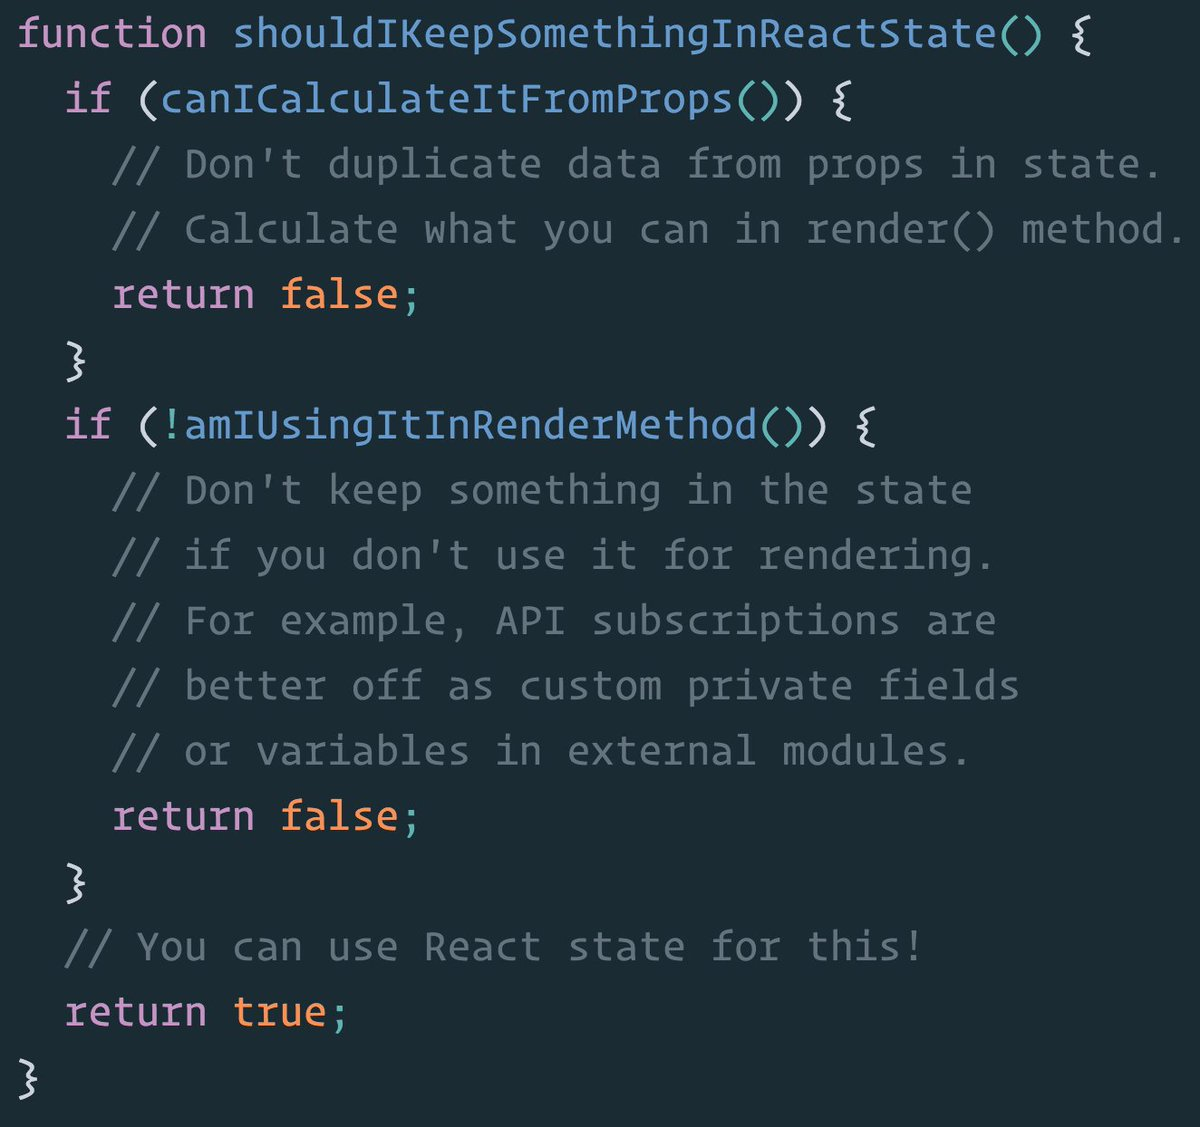
\includegraphics[width=.8\textwidth]{images/dan-cheat-sheet}
\end{figure}


\section{Prop types}

Мы ставим перед собой цель, создавать переиспользуемые компоненты, поэтому нам нужно описывать интерфейс этих компонент удобным для пользователей этих компонент образом.

React из коробки позволяет нам описывать, какие параметры ожидает компонент и простые правила валидации к ним. Привила позволяют указывать, какого типа данных должны быть параметры, а также являются ли параметры обязательными. Помимо этого React позволяет определять пользовательские функции проверки параметров.

Посмотрим на простой пример:

\begin{lstlisting}
const Button = ({ text }) => <button>{text}</button>
Button.propTypes = {
  text: React.PropTypes.string,
}
\end{lstlisting}

В этом примере мы создаем простую компонент-функцию, которая должна получать один параметр $text$, который должен быть типа $string$.

Теперь каждый, кто попытается воспользоваться данным компонентом, сможет легко понять, что ему нужно передавать даже без детального чтения кода.

Но что если компонент вообще не сможет работать, если ему не передать определенный параметр? В этом случае этот параметр можно указать как обязательный:

\begin{lstlisting}
Button.propTypes = {
  text: React.PropTypes.string.isRequired,
}
\end{lstlisting}

В этом случае кто-либо, кто создаст такой компонент, не передав обязательный параметр, получат следующую ошибку:

\begin{quotation}
\textbf{Failed prop type: Required prop `text` was not specified in `Button`.}
\end{quotation}

Важно понимать, что предупреждение об ошибке мы получим только в режиме разработки. В релизной сборке валидация с $propTypes$ выключается в целях улучшения производительности.

React предоставляет возможность проверки множества типов параметров: от чисел до массивов и компонент.

Если мы хотим, чтобы компонент работал с данными разных типов, передаваемых через один параметр, то можем использовать функцию \textbf{oneOf}, которая позволяет указать список разных типов для одного параметра.

Также стоит стараться передавать через параметры только примитивные типы, так как они лучше поддаются отладке и терстированию.

Передача примитивов также позволяет быстрее находить разбухающие интерфейсы у компонент. Если компонент начинает требовать все больше и больше параметров, то возможно он содержит больше логики чем должен и нарушает принцип единственности ответственности.

Если мы замечаем, что компонент получает множество параметров, которые слабо связаны логикой приложение, то можно попробовать разделить этот компонент на два независимых.

Однако нам все равно достаточно часто приходится передавать компонентам объекты. В этом случае для валидации следует использовать функцию $shape$.

Функция $shape$ позволяет определить параметр типа объект, а также определить тип всех полей, которые должны быть у этого объекта, которые в свою очередь тоже могут быть объектами.

Например, если мы создадим компонент $Profile$, который ожидает объект с именем и фамилией пользователя, то мы можем создать следующие $propTypes$:

\begin{lstlisting}
const Profile = ({ user }) =>(
  <div>{user.name} {user.surname}</div>
)
Profile.propTypes = {
  user: React.PropTypes.shape({
    name: React.PropTypes.string.isRequired,
    surname: React.PropTypes.string,
  }).isRequired,
}
\end{lstlisting}

Если же ни одного из стандартных методов валидации React нам не подходят, то мы можем определить собственную функцию проверки:

\begin{lstlisting}
user: React.PropTypes.shape({
  age: (props, propName) => {
    if (!(props[propName] > 0 && props[propName] < 100)) {
      return new Error(`${propName} must be between 1 and 99`)
    }
    return null
  },
})
\end{lstlisting}

Например, в примере выше мы проверяем, что возраст находится в определенном числовом промежутке. Если же возраст выйдет за этот промежуток, то мы увидим соответствующую ошибку в консоли.

\subsection*{React Docgen}

Хорошо описанные $propTypes$ уже значительное облегчение жизни тем, кто будет пользоваться нашими компонентами. Но мы можем пойти дальше и еще больше упростить их использование.

Когда количество компонентов значительно возрастает, то появляется проблема поиска необходимого компонента среди многих, особенно для новых членов проекта.

Но если мы поддерживали $propTypes$ в хорошем состоянии, то мы можем автоматически создавать из них документацию.

Для этого мы можем использовать библиотеку $react-docgen$, которую можно установить следующей командой:

\begin{lstlisting}
npm install --global react-docgen
\end{lstlisting}

React Docgen проходит по файлу с компонентом и достает, необходимую для него информацию, из $propTypes$ и комментариев.

Например, если у нас есть компонент:

\begin{lstlisting}
const Button = ({ text }) => <button>{text}</button>
Button.propTypes = {
  text: React.PropTypes.string,
}
\end{lstlisting}

И мы запустим:

\begin{lstlisting}
react-docgen button.js
\end{lstlisting}

Мы получим следующий результат;

\begin{lstlisting}
{
  "description": "",
  "methods": [],
  "props": {
    "text": {
      "type": {
        "name": "string" 
      },
      "required": false,
      "description": ""
    } 
  }
}
\end{lstlisting}

Этот JSON представляет собой описание интерфейса компонента. Как вы видите, в него попали поля и их типы, описанные в $propTypes$.

Также мы можем добавить комментарий к нашему компоненту:

\begin{lstlisting}
/**
 * A generic button with text.
 */
const Button = ({ text }) => <button>{text}</button>
Button.propTypes = {
  /**
   * The text of the button.
   */
  text: React.PropTypes.string,
}
\end{lstlisting}

Если мы снова запустим Docgen, то получим:

\begin{lstlisting}
{
  "description": "A generic button with text.",
  "methods": [],
  "props": {
    "text": {
      "type": {
        "name": "string"
      },
      "required": false,
      "description": "The text of the button."
    }
  }
}
\end{lstlisting}

Теперь, с этим описанием интерфейса в формате JSON мы можем создать документацию и использовать ее внутри команды.

Результат работы Docgen имеет простой формат, поэтому не составляет никакого труда создать страницу с документацией на его основе.

Один из ярких примеров использования React Docgen - документация библиотеки $Material UI$, где вся документация создана на основе исходного кода библиотеки.


\section{Переиспользуемые компоненты}

Мы уже хорошо разобрались с тем как создавать компоненты, как использовать внутреннее состояние компонент и как сделать их переиспользуемыми с помощью $propTypes$.

Давайте теперь, вооружившись всеми полученными знаниями, попробуем сделать из непереиспользуемыех компонент переиспользуемые.

Предположим, что у нас есть компонент, который загружает список постов через API сервера и отображает их на экране.

Это упрощенный пример, но он хорошо подходит, чтобы показать все этапы создания переиспользуемого компонента.

Создадим класс посредством его наследования от React.Component:

\begin{lstlisting}
class PostList extends React.Component
\end{lstlisting}

Затем создадим конструктор и добавим загрузку данных в $componentDidMount$:

\begin{lstlisting}
constructor(props) {
  super(props)
  this.state = {
    posts: [],
  } 
}
componentDidMount() {
  Posts.fetch().then(posts => {
    this.setState({ posts })
  })
}
\end{lstlisting}

Во $state$ компонента только одно поле $posts$, в котором мы будем хранить посты и которое инициализируется пустым массивом.

В $componentDidMount$ вызывается API сервера, для получения списка постов. По окончанию запроса посты сохраняются в $state$ компонента с помощью метода $setState$.

Это распространенный паттерн загрузки данных, другие варианты детальнее мы рассмотрим в Главе 5.

$Posts$ - это вспомогательный класс, который содержит логику общения с сервером. Сейчас для нас важно только то, что этот класс имеет метод $fetch$, который возвращает $Promise$, который при успешном выполнении вернет список постов.

Теперь мы можем отобразить список постов:

\begin{lstlisting}
render() {
  return (
    <ul>
      {this.state.posts.map(post => (
        <li key={post.id}>
          <h1>{post.title}</h1>
          {post.excerpt && <p>{post.excerpt}</p>}
        </li> ))}
    </ul> 
  )
}
\end{lstlisting}

Внутри метода $render$ мы обходим все посты и для каждого создаем элемент $<li>$.

Мы полагаем, что у поста всегда есть поле $title$ и безусловно показываем его внутри $<h1>$. Поле же $post.excerpt$ мы считаем необязательным и отображаем только при наличии.

Теперь представим другой компонент. Пусть он отображает список пользователей, которые получает из $props$, а не из собственного состояния:

\begin{lstlisting}
const UserList = ({ users }) => (
  <ul>
    {users.map(user => (
      <li key={user.id}>
        <h1>{user.username}</h1>
        {user.bio && <p>{user.bio}</p>}
      </li>
      )
    )} 
  </ul>
)
\end{lstlisting}

Данный компонент отображает список пользователей очень похожим на отображение постов способом.

Отличие в том, что теперь вместо $title$ отображается $username$ и опциональное поле теперь $bio$ пользователя вместо $excerpt$ поста. 

Дублирующийся код как правило считаются плохим звоночком, так что давайте разбираться как React позволяет следовать правилу \textbf{Не повторяйся (Don't Repeat Yourself, DRY)}. Прежде всего мы можем создать отдельный компонент $List$, в который вынесем логику отображения списков, отделив ее от самих данных. Главным требованием является возможность передать ключи полей по которым мы сможем получить данные, чтобы иметь возможность брать нужные данные из разных типов объектов.

Чтобы сделать это, мы определим два параметра: $titleKey$ для передачи ключа, по которому мы получим значение для  обязательного поля, и $textKey$ для передачи ключа опционального поля.

Параметры нашего нового компонента будут выглядеть следующим образом:

\begin{lstlisting}
List.propTypes = {
  collection: React.PropTypes.array,
  textKey: React.PropTypes.string,
  titleKey: React.PropTypes.string,
}
\end{lstlisting}

Так как $List$ не будет обладать своим собственным состоянием, мы можем его создать как компонент-функцию:

\begin{lstlisting}
const List = ({ collection, textKey, titleKey }) => (
  <ul>
    {collection.map(item =>
      <Item
        key={item.id}
        text={item[textKey]}
        title={item[titleKey]}
      /> 
    )}
  </ul> 
)
\end{lstlisting}

Компонент $List$ получает через $props$ коллекцию объектов, проходит по ним и преобразует в элементы $Item$, который мы скоро реализуем. Также в дочерний элемент мы передаем $text$ и $title$, который получаем с помощью полученных ключей из элементов коллекции.

Компонент $Item$ будет максимально простым и чистым:

\begin{lstlisting}
const Item = ({ text, title }) => (
  <li>
    <h1>{title}</h1>
    {text && <p>{text}</p>}
  </li>
)

Item.propTypes = {
  text: React.PropTypes.string,
  title: React.PropTypes.string,
}
\end{lstlisting}

Таким образом мы создали два компонента с достаточно простыми интерфейсами, чтобы с их помощью отображать пользователей, посты или что-либо еще. При этом такие небольшие компоненты очень удобны в поддержке и тестировании.

Отлично, теперь мы можем переписать наши исходные компоненты с использованием новых вспомогательных компонент.

Метод $render$ компонента $PostsList$ будет выглядеть следующим образом:

\begin{lstlisting}
render() {
  return (
    <List
      collection={this.state.posts}
      textKey="excerpt"
      titleKey="title"
    />
  )
}
\end{lstlisting}

А компонент-функция $UserList$ следующим:

\begin{lstlisting}
const UserList = ({ users }) => (
  <List
    collection={users}
    textKey="bio"
    titleKey="username"
  /> 
)
\end{lstlisting}

Таким образом мы из узкоспециализированных компонент получили базовые компоненты, которые могут быть переиспользованы в будущем.

Мы также можем использовать $react-docgen$ для генерации документации для полученных нами компонент.

Также теперь в случае необходимости расширения данного отображения, которое пока состоит из двух текстовых полей, нам будет достаточно поменять его в одном компоненте $Item$, а не в множестве узкоспециализированных компонент.

Например, если нам понадобится в случае слишком длинной строки урезать ее и показывать троеточие, нам будет достаточно добавить эту логику внутрь одного компонента.

\section{Living style guides}

Использование переиспользуемых компонент с простыми интерфейсами - хороший способ сократить количество дублирующегося кода в проекте, но это не единственная причина, чтобы сосредоточиться на переиспользуемости.

Если вы создаете простые и понятные компоненты с чистыми интерфейсами, которые хорошо отделены абстракциями от конкретных данных, то эти компоненты можно объединить в библиотеку компонент и использовать за пределами команды. Такая библиотека будет представлять из себя набор готовых к использованию блоков, которыми можно будет поделиться с другими командами, дизайнерами или выложить ее в open source.

Очень часто новым членам команды может быть сложно понять, какие компоненты уже есть, а какие нужно реализовать. Решением этой проблемы может быть создание Style guide'а, которое бы позволило распространять не только сами компоненты, но и примеры их использования.

По сути style guide - это собранное визуальное представление всех единичных компонентов, которые уже реализованы в проекте. Это очень удобный способ сохранять единый стиль всех компонент среди множества разработчиков разного уровня. 

К сожалению, создание style guide'а не всегда является простой задачей, так как из-за меняющихся требований может появиться множество дублирующихся компонент с небольшими отличиями, решающие какие-то локальные проблемы. Тем не менее React позволяет без значительных усилий создавать такой род документации, что может окупить немало времени в будущем.

Но не только React может вам помочь создать библиотеку визуальных компонентов из кода самих компонент. Есть инструменты, которые помогают решить эту проблему, один из которых $react-storybook$.

React Storybook изолирует компоненты, предоставляя вам возможность создавать компоненты без запуска всего приложения, что помогает в тестировании и разработке.

Как видно из названия библиотеки React Storybook позволяет создавать истории для отображения разных состояний компонента. Например, если вы пишите TO-DO приложение, то вы можете создать две истории для отображения выбранного и невыбранного состояний элемента.

Давайте попробуем применить эту библиотеку к примеру с компонентом $List$. Прежде всего нам нужно установить Storybook:

%npm install --save @kadira/react-storybook-addon

Теперь мы можем начать создавать истории.

В нашем примере компонент $Item$ требует обязательный параметр $title$ и опциональный $text$, в этом случае мы можем создать как минимум две истории.

Обычно истории хранят в директории $stories$ внутри проекта, но в целом никто не запрещает использовать любую удобную для вас директорию.

Внутри этой директории можно создать специально файл для каждой из компонент.

В нашем случае создадим файл $list.js$. В этом файле обязательно необходимо добавить импорт основной функции библиотеки:

\begin{lstlisting}
import { storiesOf } from '@kadira/storybook'
\end{lstlisting}

Дальше мы можем создать истории следующим образом:

\begin{lstlisting}
storiesOf('List', module)
  .add('without text field', () => (
    <List collection={posts} titleKey="title" />
  ))
\end{lstlisting}

Функция $storiesOf$ принимает аргументом название компонента и позволяет добавить для него множество историй. Каждая история включает в себя описание и функцию, которая создает необходимый компонент.

В нашем случае $posts$ может быть объектом вида:

\begin{lstlisting}
const posts = [
  {
    id: 1,
    title: 'Create Apps with No Configuration',
  },
  {
    id: 2,
    title: 'Mixins Considered Harmful',
  },
]
\end{lstlisting}

Перед запуском Storybook и создания нашей визуальной коллекции нам необходимо настроить библиотеку. Для этого необходимо создать директорию $.storybook$. 

Внутри этой директории нам нужно создать файл $config.js$ для загрузки наших историй:

\begin{lstlisting}
import { configure } from '@kadira/storybook'
function loadStories() {
  require('../src/stories/list')
}
configure(loadStories, module)
\end{lstlisting}

Сначала мы загружаем функцию $configure$ из библиотеки, а затем описываем функцию для загрузки историй по путям к их файлам.

И последний шаг, если мы хотим, чтобы storybook с нашими компонентами был доступен из браузера, мы можем добавить специальный скрипт в package.json:

\begin{lstlisting}
"storybook": "start-storybook -p 9001"
\end{lstlisting}

Теперь мы можем запустить storybook:

\begin{lstlisting}
npm run storybook
\end{lstlisting}

И открыть в браузере $http://localhost:9001$.

Теперь мы можем увидеть интерфейс storybook. Слева находится список наших историй. Если мы нажмем на историю, то справа увидим соответствующий ей компонент.

Отлично, теперь у нас есть визуальная документация наших компонент, чтобы все члены команды, в том числе продуктовые менеджеры и дизайнеры, имели представление о существующей базе готовых компонентов.

В завершение мы можем создать еще одну историю.

Наш лист умеет отображать элементы с $title$ и $text$, поэтому добавим второй атрибут в список постов:

\begin{lstlisting}
const posts = [
  {
    id: 1,
    title: 'Create Apps with No Configuration',
    excerpt: 'Create React App is a new officially supported...',
  }, 
  {
    id: 2,
    title: 'Mixins Considered Harmful',
    excerpt: '"How do I share the code between several...',
  }
]
\end{lstlisting}

После этого добавим еще одну историю, где передадим оба параметра:

\begin{lstlisting}
.add('with text field', () => (
  <List collection={posts} titleKey="title" textKey="excerpt" />
))
\end{lstlisting}

Если мы сейчас вернемся в браузер, то увидим, что наша страница автоматически обновилась, и добавилась вторая история.

Таким образом для сложных компонентов мы можем добавить любое количество историй, чтобы показать все состояния, в которых они могут находиться.

\section{Заключение}

Поздравляю, мы разобрались с созданием переиспользуемых компонент.

В этой главе мы детально посмотрели как можно создавать компоненты и в чем различие между компонент-функциями и компонентами с внутренним состоянием. Также мы изучили как осуществляется изменение состояния React компонент и как это приводит к перерисовке компонента. Помимо этого мы посмотрели как описывать параметры компонента и как это помогает в совместной работе надо общими элементами.

И в конце мы посмотрели на примеры превращения узкоспециализированных компонент в переиспользуемые посредством вынесения общей логики в достаточно абстрактные базовые компоненты.

Теперь пришло время посмотреть на разные техники комбинации компонентов между собой.



%\chapter{Собираем все в кучу}

В предыдущей главе мы разобрались, как создавать переиспользуемые компоненты. Теперь мы можем поговорить о том, как заставить это компоненты эффективно взаимодействовать друг с другом.

Сильной стороной React является то, что он позволяет создавать сложные интерфейсы комбинирование маленьких, тестируемых компонент. Этот подход позволяет контролировать каждый аспект приложения.

В этой главе мы рассмотрим самые распространенные паттерны и инструменты для комбинирования компонент.

Мы обсудим следующие вопросы:

\begin{itemize}
  \item Как компоненты коммуницируют друг с другом посредство передачи $props$ дочерним элементам
  \item Как паттерн Контейнер и Представление помогает писать более поддерживаемый код
  \item Проблему, которую пытались решить миксины (mixins), но не смогли
  \item Улучшение структуры приложения с Компонентами Высшего порядка
  \item Библиотеку recompose и ее встроенные функции
  \item Как мы можем взаимодействовать с контекстом и как избежать сильной связности компонентов с ним
  \item Паттерн Function as a Child и какую пользу он может принести
\end{itemize}


\section{Взаимодействие компонентов}

\textbf{Переиспользуемые компоненты} могут использоваться внутри множества других компонент в процессе разработки вашего приложения.

Небольшие компоненты с простым интерфейсом могут составлять более сложные компоненты, которые в свою очередь являются частью еще более сложных компонент и приложения в целом.

Мы уже неоднократно видели, как в React объединяются компоненты. Для этого достаточно описать структуру из вложенных компонент внутри метода $render$:

\begin{lstlisting}
const Profile = ({ user }) => (
  <div>
    <Picture profileImageUrl={user.profileImageUrl} />
    <UserName name={user.name} screenName={user.screenName} />
  </div>
)
Profile.propTypes = {
  user: React.PropTypes.object,
}	
\end{lstlisting}

Например вы можете создать компонент $Profile$ путем комбинирования компонентов $Picture$ для отображения изображения профиля и $UserName$ для имени пользователя.

Таким образом вам требуется всего нескольких строчек кода для добавления новых блоков интерфейса.

После того как вы объединили компоненты как на примере выше, вы можете передавать между ними данные, используя $props$.

Props - основной способ передачи данных от родительских компонент дочерним в React. 

Когда компонент передает данные другому компоненту, он является \textbf{Владельцем (Owner)} этого компоненты, не зависимо от иерархической принадлежности каждого из них.

Например, в последнем примере $Profile$ не является непосредственным родителем $Picture$ (между ними еще тег $div$), но $Profile$ является владельцем $Picture$, так как передает ему данные через параметры (прим.пер. далее я все равно буду называть такие компоненты родительскими, просто в чуть более обобщенном значение).


\subsection*{Children}

Есть специальный параметр \textbf{children}, который передается от родительского компонента дочерним и доступен в методе render.

В документации React говорится, что это \textit{непрозрачный (opaque)} параметр, так как он не несет никакой информации о том, что именно внутри него содержится.

Вложенные компоненты, определенные в методе $render$, обычно получают параметры через атрибуты в JSX (или через второй аргумент метода $createElement$).

Также компонент можно определить с вложенными компонентами, в этом случае они будут доступны для него через параметр $children$.

Представим, что у нас есть компонент $Button$, у которого есть параметр $text$, отвечающий за текст на кнопке:

\begin{lstlisting}
const Button = ({ text }) => (
  <button className="btn">{text}</button>
)
Button.propTypes = {
  text: React.PropTypes.string,
}	
\end{lstlisting}

Этот компонент можно использовать следующим образом:

\begin{lstlisting}
<Button text="Click me!" />
\end{lstlisting}

Теперь предположим, что мы хотим использовать ту же самую кнопку с тем же className, но отображать внутри нее что-то более сложное чем просто текст.

Что если мы хотим, чтобы у нас были кнопки с текстом, кнопки с изображением и кнопки с текстом и заголовком?

В множестве случаем достаточным решением будет добавить множество параметров в компонент $Button$ или создать специализированные компоненты, например $IconButton$.

Однако, если мы понимаем, что $Button$ всего лишь обертка, которая должна отображать любое содержимое, то мы можем использовать параметр $children$.

Мы можем легко поправить предыдущий вариант $Button$, чтобы иметь возможность отображать любое содержимое:

\begin{lstlisting}
const Button = ({ children }) => (
  <button className="btn">{children}</button>
)
Button.propTypes = {
  children: React.PropTypes.array,
}
\end{lstlisting}

Теперь мы можем использовать любые компоненты внутри $Button$, они будут подставлены вместо $children$ в JSX. 

Например мы можем создать кнопку с изображением и текстом внутри:

\begin{lstlisting}
<Button>
  <img src="..." alt="..." />
  <span>Click me!</span>
</Button>
\end{lstlisting}

В этом случае мы получим следующий HTML код:

\begin{lstlisting}
<button className="btn">
  <img src="..." alt="..." />
  <span>Click me!</span>
</button>
\end{lstlisting}

Это очень удобный способ, чтобы позволить компонентам принимать любые дочерние элементы и оборачивать их предопределенным образом.

Как вы могли заметить в предыдущем примере, мы определили параметр $children$ как массив, что значит, что можно передать любое количество элементов.

Но если мы передадим только один элемент, например:

\begin{lstlisting}
<Button>
  <span>Click me!</span>
</Button>
\end{lstlisting}

то получим следующую ошибку:

\begin{quote}
	\textbf{ Failed prop type: Invalid prop `children` of type `object` supplied to `Button`, expected `array`.} (Неверный тип параметра: неверный тип параметра 'children' с типом 'объект', переданный компоненту $Button$; ожидается 'массив' )
\end{quote}

Это происходим из-за того, что в случае с передачей одиночного элемента React оптимизирует выделение памяти и используем сам элемент вместо создания массива с одним элементом.

Мы можем легко это поправить, указав в propTypes не только массив, но и одиночный элемент:

\begin{lstlisting}
Button.propTypes = {
  children: React.PropTypes.oneOfType([
    React.PropTypes.array,
    React.PropTypes.element,
  ]),
}
\end{lstlisting}

\section{Паттерн Контейнер и Представление}

В этой главе мы рассмотрим паттерн, который поможет сделать наш код еще чище и более поддерживаемым.

Как правило React компоненты представляют из себя сочетание \textbf{логики} и \textbf{отображения}.

Под логикой мы понимаем все, что не относится к UI, т.е. такие вещи как обращения к API сервера, преобразование данных и обработку событий.

А под представлением наоборот, ту часть, которая отвечает за создание элементов для UI. Прежде всего это содержимое метода $render$.

В React есть простой и мощный паттерн, \textbf{Контейнер и Представление (Container and Presentational)}, который помогает разделить по отдельным компонентам две эти составляющие.

Заодно посмотрим в этой главе, какая еще польза, помимо переиспользуемости компонент, может быть от разделения логики и представления.

Как всегда начнем изучения паттерна с примера, в котором он используется.

Предположим, у нас есть компонент, который получает из API геолокации долготу и широту, а затем отображает их на экране.

Для начала создадим файл $geolocation.js$ и определим в нем компонент $Geolocation$:

\begin{lstlisting}
class Geolocation extends React.Component
\end{lstlisting}

В этом компоненте создадим конструктор для определения начального состояния и привязки обработчиков событий:

\begin{lstlisting}
constructor(props) {
  super(props)
  this.state = {
    latitude: null,
    longitude: null,
  }
  this.handleSuccess = this.handleSuccess.bind(this)
}
\end{lstlisting}

Теперь в $componentDidMount$ мы можем осуществить вызов API:

\begin{lstlisting}
componentDidMount() {
  if (navigator.geolocation){     
    navigator.geolocation.getCurrentPosition(this.handleSuccess)
  }
}
\end{lstlisting}

После того, как компонент получит данные от сервера, их можно сохранить во внутреннее состояние компонента:

\begin{lstlisting}
handleSuccess({ coords }) {
  this.setState({
    latitude: coords.latitude,
    longitude: coords.longitude,
  })
}
\end{lstlisting}

И в конце концов мы можем отобразить высоту и широту на экране через метод $render$:

\begin{lstlisting}
render() {
  return (
    <div>
      <div>Latitude: {this.state.latitude}</div>
      <div>Longitude: {this.state.longitude}</div>
    </div> 
  )
}
\end{lstlisting}

Важно заметить, что после первой отрисовки компонента значение долготы и широты равно $null$, так как запрос на данные асинхронен и лишь инициализируется в $componentDidMount$. В реальном проекте вы скорее всего захотите в этот момент показывать какой-то индикатор загрузки, что можно сделать с помощью условных операторов, подробно разобранных в Главе 2.

Но в целом в этом компоненте нет никаких проблем и он прекрасно работает.

Предположим, что мы работаем с дизайнером над UI составляющей компонента. Не было бы это хорошей идеей, создать компонент, состоящий только из UI части, чтобы иметь возможность быстрее обсудить ее с дизайнером.

 Если мы отделим представление от логики, то мы сможем без проблем добавить его в документацию на основе \textbf{Storybook}, как мы делали в одной из предыдущих глав.
 
 Как вы уже можете догадаться, использование паттерна Контейнер и Представление предполагает разделение компонента на два, с более четкой зоной ответственности у каждого.
 
 Если быть более точным, то в Контейнере находится вся логика и работа с данными, а в Представлении создание элементов и минимум логики. Чаще всего компонент представления может быть выражен компонент-функцией.
 
 Но это не значит, что в Представлении не может быть состояния вообще. В некоторых случаях, например при создании полей ввода, может быть уместнее хранить состояние в компоненте представления.
 
 В случае нашего примера мы отображаем на экране лишь широту и долготу, поэтому мы воспользуемся компонент-функцией для создания Представления.
 
 Для начала переименуем наш компонент $Geolocation$ в $GeolocationContainer$:
 
\begin{lstlisting}
class GeolocationContainer extends React.Component
\end{lstlisting}

А также переименуем файл, содержащий этот компонент, из $geolocation.js$ в $geolocation-container.js$.

Такой вариант наименования не высечен в камне, но является наиболее распространенным в сообществе React. К компоненты Контейнера мы добавляем в конце $Container$, а компоненте Представления оставляем оригинальное имя.

Также нам нужно изменить реализацию метода $render$, заменив все содержимое отрисовкой одного компонента:

\begin{lstlisting}
render() {
  return (
    <Geolocation {...this.state} />
  )
}
\end{lstlisting}

Таким образом, вместо отрисовки HTML элементов мы просто отображаем компонент Представления и передаем в него свое состояние.

В \textbf{состоянии} нашего компонента высота и широта, которые по умолчанию имеют значение $null$ и меняются на координаты пользователя через \textbf{обратный вызов (calback)} после вызова API.

Чтобы передать состояние целиком, мы используем спред оператор (spread operator), который избавляет нас от необходимости указывать параметры один за другим вручную.

Теперь создадим файл $geolocation.js$, в котором создадим компонент Отображения:

\begin{lstlisting}
const Geolocation = ({ latitude, longitude }) => (
  <div>
    <div>Latitude: {latitude}</div>
    <div>Longitude: {longitude}</div>
  </div>
)
\end{lstlisting}

Компонент-функции - очень лаконичный способ описания интерфейса. Чистые функции однозначно отображают состояние в набор элементов.

В нашем случае компонент принимает через $state$ долготу и широту и отображет их внутри $div$ элементов.

Мы хотим следовать лучшим практикам, поэтому определим необходимый и достаточный интерфейс для этого компонента:

\begin{lstlisting}
Geolocation.propTypes = {
  latitude: React.PropTypes.number,
  longitude: React.PropTypes.number,
}	
\end{lstlisting}

Следуя паттерну Контейнер и Представление, мы сорздаем глупые компоненты, которые потом можно использовать в Style guide с искусственными данными.

Если в нашем приложении в другом месте будет предполагаться такой же визуальный компонент, то нам не придется создавать компонент с нуля. Нам будет достаточно создать новый Контейнер для существующего представления, например если нам нужно будет загрузить координаты из другого сервиса.

Также другим членам команды будет проще расширить логику в контейнере, например добавить обработку ошибок, не затрагивая представления.

Также можно создать временный компонент с отображением отладочной информации для скорейшей реализации логики.

Также такой подход позволяет разделить создание компонента между разными людьми, что особенно полезно в случае больших команд и итеративных процессов разработки.

Это очень простой в использовании и полезный на практике паттерн. В большой команде он способен значительно увеличить скорость разработки и поддерживаемость написанного кода.

Но с другой стороны, использование этого паттерна без явной необходимости может значительно увеличить количество файлов и размер кодовой базы.

Не стоит начинать делить все компоненты на два сломя голову. Чаще всего стоит начинать рефакторить компонент посредством разделения логики и представления, когда они начинают быть сильно связанными. 

Например в нашем примере, мы предположили, что у нас может появиться другой источник данных, для которого мы и будем создавать отдельный компонент.

Не всегда можно однозначно понять, что должно быть в Контейнере, а что в Представлении. Следующий список утверждений должен помочь вам в сложной ситуации:

Компонент Контейнера:

\begin{itemize}
  \item Сосредоточен больше на поведении
  \item Отображает компонент Представления
  \item Выполняет асинхронные запросы к серверу и преобразует данные
  \item Определяет обработчики событий
  \item Создаются как наследуемые от React.Component классы
\end{itemize}


Компонент Представления:

\begin{itemize}
  \item Сконцентрированы на визуальной составляющей 
  \item Отображают HTML разметку (и другие компоненты)
  \item Получают данные от родительского компонента через $props$
  \item Часто определяются через компонент-функции без состояния
\end{itemize}


\section{Mixins}

Компоненты отлично служат цели достижения переиспользуемости кода, но что если у нас появляется множество различных компонент, которые должны обладать общими чертами?

Очевидно, мы не хотим дублировать код, к счастью React предоставляет специальный инструмент для решения этой проблемы: \textbf{примеси (mixins)}.

В общем и целом примеси не рекомендуются к использованию, но все равно стоит знать, какие проблемы они решают и какие есть альтернативы.

Также есть не нулевая вероятность, что вас может занести на проект с кучей старого кода, где могут во всю применяться примеси, поэтому быть готовым к такому повороту лишним не будет.

Начать стоит с того, что примеси работают только с $createClass$, что является одной из причин предания их забвению.

Предположим, что вы используете $createClass$ и понимаете, что вам нужно написать один и тот же код в разные компоненты.

Например, вам нужно подписаться на событие изменения размера экрана и выполнять по нему какой-то код.

Собственно его можно написать один раз и передавать через примеси в любые компоненты. Посмотрим на примере кода.

Точкой соприкосновения компонента и примеси обычно выбирается $state$. Мы можем выделить в $state$ конкретное поле и использовать его и из компонента и из примеси. В остальном примесь описывается как обычный самостоятельный компонент.

Определим в нашей примеси начальное состояние с помощью метода $getInitialState$, в котором будет одно поле $innerWidth$:

\begin{lstlisting}
getInitialState() {
  return {
    innerWidth: window.innerWidth,
  }
},
\end{lstlisting}

Теперь мы можем начать отслеживать изменения размера экрана, для чего подпишемся на соответсвующее событие:

\begin{lstlisting}	
componentDidMount() {
  window.addEventListener('resize', this.handleResize)
},
\end{lstlisting}

Также мы хотим удалить этот обработчик события перед удалением компонента, чтобы избежать накопления неиспользуемых обработчиков в объекте $window$:

\begin{lstlisting}
componentWillUnmount() {
  window.removeEventListener('resize', this.handleResize)
},
\end{lstlisting}

И осталось только создать функцию, которая будет вызваться на каждом изменении размера экрана.

В этой функции мы будем обновлять значение поля $innerWidth$ в $state$ актуальным значением, так что любой компонент, который использует эту примесь, будет перерисован как после собственного $setState$:

\begin{lstlisting}
handleResize() {
  this.setState({
    innerWidth: window.innerWidth,
  })
},
\end{lstlisting}

Как видно из примера, создание примеси почти не отличается от создания обычного компонента.

Чтобы использовать эту примесь вместо с компонентом, достаточно добавить ее в массив $mixins$ внутри компонета:

\begin{lstlisting}
const MyComponent = React.createClass({
  mixins: [WindowResize],
    render() {
      console.log('window.innerWidth', this.state.innerWidth)
      ...
  }, 
})
\end{lstlisting}

С этого момента значение $innerWidth$ будет доступно не только в примеси, но и в компоненте, который будет перерисовывать при каждом обновлении состояния из примеси.

Само собой мы можем использовать одну и ту же примесь в множестве компонент, также и внутри одного компонента может использоваться сразу множество примесей.

Очень полезной особенностью примесей является то, что они обладают одинаковым с компонентами жизненным циклом, а также возможностью задать состояние по умолчанию.

Например, если мы используем $WindowResize$ в компоненте, в котором уже есть $componentDidMount$, то никаких коллизий не произойдет, и оба метода выполнятся.

Теперь посмотрим, в чем проблемы примесей и почему от них отказались. А в следующей части разберемся, как достигнуть такого же результата другими средствами.

Во первых примеси часто используют внутренние функции для взаимодействия с компонентом.

Например, наша примесь $WindowResize$ может ожидать, что функция обратного вызова $handleResize$ будет реализована внутри компонента, что даст возможность разработчикам большую свободу в обработке изменения размера экрана.

Или наоборот, примесь хочет получать данные из компонента и дергает специальный метод, что-то вроде $getInnerWidth$. Само собой этот метод тоже должен быть реализован внутри компонента.

К сожалению, нет никакой возможности получить точный список методов, которые должны быть реализованы внутри компонента при добавлении примеси.

Такой подход очень сильно ухудшает поддерживаемость кода. Если компонент использует множество примесей, то при их удалении или изменении очень сложно выделить код, которые также может быть удален или требует модификации.

Также частая проблема - конфликты имен. Очень часто примеси могут начать требовать функции или атрибуты с одинаковыми названиями. React без проблем разделяет вызовы методов жизненного цикла компонент, но совсем ничего не может сделать с вызовами пользовательских функций.

Таким образом примесям остается использовать внутреннее состояние компонент, что не очень хорошо, так как мы пытаемся наоборот сократить его использование с целью повышения переиспользуемости.

Помимо этого, может начать складываться ситуация, когда одни примеси начинают зависеть от других. Например, мы можем создать еще одну примесь \textbf{ResponsiveMixin}, которая будет скрывать некоторые элементы с экрана в зависимости от текущего размера экрана, который мы получаем из примеси $WindowResize$.

Такая тесная связь примесей значительно усложняет отладку приложения и его масштабируемость. 

\section{Компоненты высшего порядка}

В прошлой части мы посмотрели, как примеси помогают избежать дублирования кода при создании общего для компонент функционала, и какие проблемы это приносит.

Когда мы говорили о функциональном программировании в Главе 2, мы упоминали концепцию \textbf{Функций высшего порядка (Higher-order Functions, HoFs)}. Такая функция принимает аргументом другую функцию и возвращает ее с измененным поведением.

Посмотрим, можем ли мы применить этот подход к React компонентам и достигнуть цели переиспользования функционала множеством компонент.

В случае применения данной концепции к компонентам React они станут называться \textbf{Компонентами высшего порядка (Higher-order Components, HoCs)}

Структура любого HoC выглядит следущим образом:

\begin{lstlisting}
const HoC = Component => EnhancedComponent
\end{lstlisting}

Компонент высшего порядка - это функция, которая принимает аргументом React компонент и возвращает его с расширенным функционалом.

Давайте начнем с простого примера, чтобы как это все выглядит на практике.

Предположим, что вам по какой-то причине необходимо добавить к множеству компонент один и тот же $className$. Никто не запрещает обойти все компоненты и в каждом поправить метод $render$, а можно создать один HoC, который решит нашу проблему:

\begin{lstlisting}
const withClassName = Component => props => (
  <Component {...props} className="my-class" />
)
\end{lstlisting}

Если вы впервые встречаете эту концепцию, может быть не очевидно, как работает этот код, поэтому давайте детально разбираться, что тут происходит.

Мы определили функцию $withClassName$, которая принимает аргументом компонент $Component$ и возвращает другую функцию.

Эта созданная функция есть обыкновенная компонент-функция, которая принимает аргументом параметры $props$ и возвращает компонент $Component$, передавая ему с помощью спред оператора все параметры и в дополнение к ним параметр $className$ со значением $"my-class"$. 

Чаще всего HoC передают параметры дальше через спред оператор. Это делается для того, чтобы HoC меньше зависел от изменения API компонента, а также чтобы только добавлять поведение и минимально затрагивать поведение самого компонента.

Это очень простой пример, который скорее всего никогда не пригодился бы в реальном проекте, но на нем мы посмотрели как выглядит HoC и как его можно создать.

Теперь посмотрим, как $withClassName$ можно использовать с другими компонентами.

Прежде всего создадим компонент, который принимает в параметрах $className$ и добавляет его к $div$ элементу:

\begin{lstlisting}
const MyComponent = ({ className }) => (
  <div className={className} />
)
MyComponent.propTypes = {
  className: React.PropTypes.string,
}
\end{lstlisting}

Но вместо того, чтобы использовать этот компонент напрямую, мы передадим его созданному ранее HoC'у, и по сути получим новый компонент:

\begin{lstlisting}
const MyComponentWithClassName = withClassName(MyComponent)
\end{lstlisting}

Оборачивая наш компонент в $withClassName$, мы гарантируем получение компонентом параметра $className$.

Давайте теперь попробуем сделать что-то более впечатляющее и переделаем примесь $WindowResize$ из предыдущей части в HoC, чтобы снова иметь возможность переиспользоввать ее в сферическом проекте в вакууме.

Напомним, что эта примесь создавала обработчик для отслеживания изменения размера экрана и сохраняла актуальное значение в поле $innerWidth$ внутри состояния компонента.

Основная проблема была в том, что примесь использовала $state$ компонента, чтобы передавать ему актуальные данные.

Это не очень хорошее поведение, так как могут возникнуть конфликты имен внутри состояния компонента.

Прежде всего создадим функцию, которая принимает аргументом компонент:

\begin{lstlisting}
const withInnerWidth = Component => (
  class extends React.Component { ... }
)
\end{lstlisting}

Возможно вы обратили наименование HoC. Это распространенная практика начинать название с $with$, если HoC расширяет параметры, которые передаются компоненту.

Помимо этого, $withInnerWidth$ будет возвращать компонент-класс, а не компонент-функцию, так как нам потребуется использовать внутреннее состояние и методы жизненного цикла.

Посмотрим, как будет выглядеть возвращенный класс.

В конструкторе мы определим начальное состояние и привяжем функцию обработчика событий к создаваемому экземпляру класса:

\begin{lstlisting}
constructor(props) {
  super(props)
  this.state = {
    innerWidth: window.innerWidth,
  }
  this.handleResize = this.handleResize.bind(this)
}
\end{lstlisting}

Добавление и удаление обработчиков события изменения размера экрана и обновление внутреннего состояния аналогично уже реализованному в примеси:

\begin{lstlisting}
componentDidMount() {
  window.addEventListener('resize', this.handleResize)
}
componentWillUnmount() {
  window.removeEventListener('resize', this.handleResize)
}
handleResize() {
  this.setState({
    innerWidth: window.innerWidth,
  })
}
\end{lstlisting}

И в конце нам нужно реализовать метод $render$, в котором мы должны отобразить изначальный компонент, передавая ему новые данные:

\begin{lstlisting}
render() {
  return <Component {...this.props} {...this.state} />
}
\end{lstlisting}

Можно обратить внимание, что мы через спред оператор передаем не только параметры, но также и внутреннее состояние.

По сути мы аналогично примеси храним $innerWidth$ внутри состояния, но передаем его не в $state$ изначального параметра, а в его $props$.

Как мы уже говорили в Главе 3, использование параметров чаще всего предпочтительнее состояния в разрезе повышения переиспользуемости компонент.

Теперь мы можем без проблем обернуть любой компонент, который ожидает параметр $innerWidth$ (или не ожидает, но зачем тогда все это..) в $withInnerWidth$ HoC.

Создадим для примера компонент, который получает параметр $innerWidth$ и просто выводит его значение на экран:

\begin{lstlisting}
const MyComponent = ({ innerWidth }) => {
  console.log('window.innerWidth', innerWidth)
  ...
}
MyComponent.propTypes = {
  innerWidth: React.PropTypes.number,
}
\end{lstlisting}

Который мы можем теперь обернуть функцией $withInnerWidth$ следующим образом:

\begin{lstlisting}
const MyComponentWithInnerWidth = withInnerWidth(MyComponent)
\end{lstlisting}

Есть несколько преимуществ использования этого подхода перед примесями: прежде всего мы не затрагиваем внутреннее состояние исходного компонента, а также не требуем (и не ожидаем) от него реализации каких-либо специфичных методов.

Это значит, что и исходный компонент и компонент высшего порядка не связаны, что позволяет переиспользовать их независимо друг от друга в дальнейшем.

Также передача данных через параметры позволяет уменьшить количество логики внутри исходного компонента, что упрощает его использование внутри Style Guide. 

В этом случае нам достаточно создать компонент с разными размера экрана, которые мы поддерживаем внутри приложения.

Т.е. мы без проблем можем передать конкретное число в через параметры так:

\begin{lstlisting}
<MyComponent innerWidth={320} />	
\end{lstlisting}

Или так:

\begin{lstlisting}
<MyComponent innerWidth={960} />	
\end{lstlisting}


\section{Recompose}

В предыдущей главе мы познакомились с компонентами высшего порядка и на примерах посмотрели, как они работают.

Есть библиотека, которая называется \textbf{recompose}, которая предоставляет набор полезных HoC, а также удобный способ их комбинировать.

Библиотечные HoC представляют из себя простые вспомогательные компоненты, которые помогают вынести часть логики из компонент, что конечно же делает их проще и более переиспользуемыми (прим. пер. за питоном не ходи, чтобы найти здесь самое переиспользуемое слово...).

Предположим, что наш компонент получает объект с данными пользователя из API, и у этого объекта есть множество атрибутов.

Получение сложного объекта компонентом в общем случае считается не самой лучшей практикой. Если компонент получает сложный объект, то скорее всего он знает о структуре этого объекта (или его части), а это ведет к том, что в случае изменения структуры этого объекта компонент будет сломан.

Будет гораздо лучше, если необходимые данные будут переданы в виде отдельных параметров с примитивными значениями.

Пусть у нас есть компонент $Profile$, в котором мы хотим отобразить $username$ и $age$:

\begin{lstlisting}
const Profile = ({ user }) => (
  <div>
    <div>Username: {user.username}</div>
    <div>Age: {user.age}</div>
  </div>
)
Profile.propTypes = {
  user: React.PropTypes.object,
}
\end{lstlisting}

Если мы хотим изменить интерфейс компонента, чтобы получать одиночные параметры вместо полного объекта, мы можем воспользоваться $flattenProp$ HoC из библиотеки recompose.

Посмотрим, как это работает.

Для начала поправим сам компонент, чтобы получать в нем одиночные параметры:

\begin{lstlisting}
const Profile = ({ username, age }) => (
  <div>
    <div>Username: {username}</div>
    <div>Age: {age}</div>
  </div>
)
Profile.propTypes = {
  username: React.PropTypes.string,
  age: React.PropTypes.number,
}
\end{lstlisting}

Теперь обернем его в $flattenProp$ HoC:

\begin{lstlisting}
const ProfileWithFlattenUser = flattenProp('user')(Profile)
\end{lstlisting}

Вы можете заметить, что мы используем этот HoC немного не так как предыдущие. Сами HoC также могут зависеть от некоторых параметров, тогда обычно сначала передают их, а потом уже компонент. В общем случае такие HoC имеют следующую структуру:

\begin{lstlisting}
const HoC = args => Component => EnhancedComponent
\end{lstlisting}

За счет этого мы можем разделить создание конкретного HoC с определенным набором параметром и использование его с копонентами:

\begin{lstlisting}
const withFlattenUser = flattenProp('user')
const ProfileWithFlattenUser = withFlattenUser(Profile)
\end{lstlisting}

Уже неплохо. Но сейчас параметры компонента завязаны на то, что это именно данные о пользователе. Давайте сделаем их более обобщенными.

В этих целях мы можем использовать $renameProp$ HoC из recompose и обновить компонент следующим образом:

\begin{lstlisting}
const Profile = ({ name, age }) => (
  <div>
    <div>Name: {name}</div>
    <div>Age: {age}</div>
  </div>
)
Profile.propTypes = {
  name: React.PropTypes.string,
  age: React.PropTypes.number,
}
\end{lstlisting}

Теперь мы можем приметь оба HoC (один для выделения простых параметров из объекта $user$ и второй для их переименования) к компоненту. Но множество вложенных вызовов функций будет ужасно читаться.

Тут нам на помощь приходит функция $compose$ библиотеки $recompose$.

Она делает очень простую вещь, принимает множество компонент высшего порядка и возвращает функцию (по сути тоже HoC), которая может применить их к какому-либо компоненту:

\begin{lstlisting}
const enhance = compose(
  flattenProp('user'),
  renameProp('username', 'name'),
  withInnerWidth
)
\end{lstlisting}

Как можете увидеть, функция $compose$ значительно улучшает читаемость кода.

Мы можем объединить множество HoC, чтобы сохранить изначальный компонент настолько простым, насколько это возможно.

Но и тут важно не переусердствовать, так как каждое добавление слоя абстракции потенциально может принести проблем, а конкретно в данном случае, множество вложенных HoC могут сказаться на производительности.

Нужно держать в голове, что добавляя каждый новый HoC, вы добавляете еще один метод $render$, еще одну пачку методов жизненного цикла и выделяете на это память.

Если у вас появляются глубокие вложенные компоненты высшего порядка, то стоит задуматься, возможно у вас что-то поломалось в структуре самого приложения.

\subsection*{Context}

Также компоненты высшего порядка очень удобны в работе с контекстом.

Контекст (Context) - инструмент библиотеки React, который используется во множестве библиотек, хотя был задокументирован значительно позже своего появления.

Документация до сих пор рекомендует при возможности не использовать контекст, так как он еще находится в стадии эксперимента и его API может в будущем измениться.

Однако этот инструмент очень полезен в случаях, когда нам нужно передать данные ниже по дереву элементов, но при этом не передавать их через каждый уровень в $props$.

Компоненты высшего порядка и контекст образуют очень мощную связку, так как позволяют передавать данные ниже по дереву, но при этом избежать сильной связи между компонентами и API контекста.

Схема проста - HoC получает данные из контекста, преобразует в $props$ и передает компоненту.

В этом случае компонент ничего не знает о существовании контекста и может быть переиспользован в любом месте приложения.

Помимо этого, в случае изменения API контекста, нам не придется исправлять все компоненты, нужно будет лишь поправить необходимые HoC.

В библиотеки recompose есть специальный метод, который делает процесс извлечения данных из контекста понятным и одинаковым для всех компонент.

Предположим, что у вас есть компонент $Price$, который вы используете для отображения валюты и величины. 
 
 Контекст часто используется для того, чтобы передавать общие настройки приложения всем компонентам, валюта может быть одной из таких настроек.
 
 Давайте начнем с компонента, который сам работает с контекстом, и шаг за шагом переделаем его в более универсальный:
 
\begin{lstlisting}
const Price = ({ value }, { currency }) => (
  <div>{currency}{value}</div>
)
Price.propTypes = {
  value: React.PropTypes.number,
}
Price.contextTypes = {
  currency: React.PropTypes.string,
}
\end{lstlisting}

У нас есть компонент-функция, которая принимает значение как параметр, а валюту вторым аргументом из контекста.

Также для обоих параметром мы определили типы (prop types и context types).

Как видим, его переиспользуемость сильно ограничивается потребностью в родительском элементе с $currency$ в контексте.

Например, мы не сможем без проблем использовать его в Style guide, так как не сможем передать валюту через параметры.

Прежде всего поменяем компонент так, чтобы он получал оба значения через параметры:

\begin{lstlisting}
const Price = ({ currency, value }) => (
  <div>{currency}{value}</div>
)
Price.propTypes = {
  currency: React.PropTypes.string,
  value: React.PropTypes.number,
}
\end{lstlisting}

Конечно, нельзя просто так взять и заменить старый компонент новым, так как нет родительского элемента, который бы передал в параметрах валюту.

Но мы можем создать специальный HoC, чтобы перенести в параметры компонента данные из контекста.

Мы будем использовать функцию $getContext$ из recompose, но ничего не мешает вам написать собственную реализацию с нуля.

Создадим отдельно сам HoC с помощью $getContext$, таким образом его можно будет переиспользовать множество раз: 

\begin{lstlisting}
const withCurrency = getContext({
  currency: React.PropTypes.string
})
\end{lstlisting}

И мы можем применить его к нашему компоненту:

\begin{lstlisting}
const PriceWithCurrency = withCurrency(Price)
\end{lstlisting}

Теперь мы можем заменить старый компонент $Prive$ новым, и компонент будет работать без явной привязки к контексту.

Для нас это большая победа, так как нам совсем не пришлось изменять родительские компоненты, но теперь мы меньше завязаны на Context API, которое может измениться, и наш компонент стал гибче в использовании.


\section{Функция как Потомок}

Есть еще один паттерн в React, о котором точно стоит знать, он называется \textbf{Функция как Потомок (Function as Child)}

Чаще всего вместе с ним вспоминают библиотеку react-motion, о которой мы подробнее поговорим в Главе 6.

Основная идея здесь заключается в том, что мы вместо того, чтобы передавать компоненту дочерние элементы, передаем ему функцию, которая сможет создать ему дочерний элемент, и в аргументах которой этот элемент сможет передать ей данные.

Посмотрим, как это выглядит:

\begin{lstlisting}
const FunctionAsChild = ({ children }) => children()
FunctionAsChild.propTypes = {
  children: React.PropTypes.func.isRequired,
}
\end{lstlisting}

Как вы видите, компонент $FunctionAsChild$ смотрит на параметр $children$ как на функцию. И вместо того, чтобы использовать его внутри JSX, вызывает его.

Этот компонент может быть использован следующим образом:

\begin{lstlisting}
<FunctionAsChild>
  {() => <div>Hello, World!</div>}
</FunctionAsChild>
\end{lstlisting}

В общем-то и весь паттерн. Мы передаем в компонент $FunctionAsChild$ функцию, которая создает текст "Hello, World!" внутри тега $div$. Эта функцию будет вызвана внутри метода $render$ компонента $FunctionAsChild$.

Смысл этот подход начинает обретать тогда, когда этой функции через аргументы будут передаваться какие-либо данные.

Создадим компонент $Name$, который ожидает в $children$ функцию и передает ей строку 'World':

\begin{lstlisting}
const Name = ({ children }) => children('World')
Name.propTypes = {
  children: React.PropTypes.func.isRequired,
}
\end{lstlisting}

Воспользоваться этим компонентом можно следующим образом:

\begin{lstlisting}
<Name>
  {name => <div>Hello, {name}!</div>}
</Name>
\end{lstlisting}

На экране будет тот же 'Hello, World!', но на этот раз имя передается не из компонента, где функция создается, а из компонента, в котором она вызывается.

Мы разобрались, как работает этот прием, давайте посмотрим, какую пользу он приносит.

Первый плюс в том, что мы можем обернуть компоненты, передавая им переменные во время исполнения программы, в отличие от фиксированных параметром, как мы делали в HoC.

Хороший пример - компонент $Fetch$, который загружает данные из сети и передает их функции $children$:

\begin{lstlisting}
<Fetch url="...">
  {data => <List data={data} />}
</Fetch>
\end{lstlisting}

Во вторых, этот подход позволяет избежать использования предустановленных имен параметров в $children$. Так как в компонент приходит функция, то их может определить разработчик, который использует этот компонент.

И также, что не менее важно, такой компонент очень удобен для переиспользования, так как он не делает никаких предположений относительно того, как будут выглядеть дочерние компоненты.

Таким образом, компонент, использующий паттерн Функция как Потомок, может быть использован в разных частях приложения с разными дочерними компонентами.

\section{Заключение}

В этой главе мы научились комбинировать наши переиспользуемые компоненты и выстраивать между ними эффективную коммуникацию.

Определение минимального и понятного интерфейса компонента через $props$ - отличный способ сделать компоненты менее связными друг с другом.

Потом мы посмотрели на самые распространенные паттерны комбинирования в React.

Первым был паттерн Контейнер и Представление, который помогает отделить логику работы компонента от его отображения и создавать узкоспециализированные компоненты, которые следуют принципу единственности ответственности.

Мы посмотрели, как React предлагает решить проблему использования общего кода между компонентами с помощью примесей. К сожаления, этот подход помимо решения проблемы, приносит множество новых, а также негативно сказывается на поддерживаемости приложения.

Один из способов достижения той же цели - использование компонент высшего порядка (HoC), которые являясь функцией, принимают аргументом компонент и возвращают его с расширенным функционалом.

Библиотека recompose предлагает множество удобных в использовании HoC, а также удобный способ их комбинирования, что позволяет вынести еще больше логики из наших компонент.

Также мы научились использовать контекст без сильной привязки к нему компонент за счет использования HoC.

И в конце мы разобрались, как связывать компоненты динамически с помощью паттерна Функция как Потомок.

Теперь пришло время, чтобы поговорить о загрузке данных из сети и об однонаправленном потоке данных. 


















%\chapter{Загрузка данных}

Цель этой главы - рассмотреть различные способы загрузки данных в React приложении.

Чтобы лучше понимать, как работать с загружаемыми данными, нам нужно будет разобраться как в целом распространяются данные по дереву компонентов в React.

Важно понимать, как родительские компоненты могут коммуницировать с потомками. А также как несвязанные между собой напрямую потомки могут передавать друг другу данные.

Мы посмотрим на конкретные примеры загрузки данных и улучшение структуры компонент, которые загружают данные, с HoC.

И в конце мы посмотрим на удобные библиотеки, такие как  react-refetch, которые могут сохранить нам много времени, предоставляя ядро работы с сетью.

В этой главе мы рассмотрим следующие пункты:

\begin{itemize}
  \item Как Однонаправленный поток данных в React упрощает для понимания структуру приложения
  \item Как дочерние элементы могут взаимодействовать с родителем через функции обратного вызова
  \item Как множество дочерних компонент могут делить данные между собой через общий родительский элемент
  \item Как создать универсальный HoC, с помощью которого можно будет загружать данные из любого API
  \item Как работает библиотека react-refetch, и как она может упростить работу с сетевыми запросами в нашем приложении
\end{itemize}


\section{Поток данных}

В последних двух главах мы разбирались, как создавать переиспользуемые компоненты и как эффективно их комбинировать.

Теперь мы поговорим о том, как выстроить правильный поток данных (data flow) между множеством компонент внутри нашего приложения.

React использует очень интересный паттерн, чтобы распространять данные от коренных элементов к дочерним. Этот паттерн обычно называют \textbf{Однонаправленный поток данных (Unidirectional Data Flow)}, и в этой части мы посмотрим на него детальнее.

Как видно из названия данные в React компонентах передаются в одном направлении, от корневых элементов к дочерним. У этого подхода есть множество преимуществ, так как это упрощает поведение компонент и их взаимоотношения, делая код более предсказуемым и поддерживаемым.

Каждый компонент получает данные от родительского компонента в виде параметров, которые не должен модифицировать. Также каждый компонент может при необходимости иметь собственное состояние. На основе состояния и полученных параметров компоненты может создать новые данные и передать их дальше по дереву элементов.

Во всех примерах, которые мы видели на текущий момент, данные передавались только от родительских компонент дочерним.

Однако, что делать, если появилась необходимость передать данные от дочернего элемента родительскому?, или родительский элемент должен быть обновлен при изменении состояния дочернего?, или два дочерних элемента хотят передать данные друг другу? Мы ответим на все эти вопросы в процессе разбора примеров из жизни.

Мы начнем с простого компонента, у которого нет потомков, и шаг за шагом преобразуем его в компонент чистый и структурированный.

Мы должны посмотреть, какие паттерны на каждом из шагов преобразования компонента подходят больше всего.

Давайте погрузимся в создание компонента счетчика $Counter$, который имеет две кнопки для увеличения и уменьшения счетчика и значению $0$ по умолчанию.

Начнем с создания класса, который наследует $React.Component$:

\begin{lstlisting}
class Counter extends React.Component
\end{lstlisting}

В конструкторе мы зададим начальное значение счетчика и привяжем к компоненту обработчики событий:

\begin{lstlisting}
constructor(props) {
  super(props)
  this.state = {
    counter: 0,
  }
  this.handleDecrement = this.handleDecrement.bind(this)
  this.handleIncrement = this.handleIncrement.bind(this)
}	
\end{lstlisting}

Обработчики событий будут также просты, им достаточно изменять состояние компонента, увеличивая или уменьшая значение счетчика:

\begin{lstlisting}
handleDecrement() {
  this.setState({
    counter: this.state.counter - 1,
  })
}
handleIncrement() {
  this.setState({
    counter: this.state.counter + 1,
  })
}
\end{lstlisting}

И в конце нам нужно создать метод $render$, в котором мы будем отображать текущее состояние счетчика и кнопки для его изменения:

\begin{lstlisting}
render() {
  return (
    <div>
      <h1>{this.state.counter}</h1>
      <button onClick={this.handleDecrement}>-</button>
      <button onClick={this.handleIncrement}>+</button>
    </div> 
  )
}
\end{lstlisting}

\subsection*{Взаимодействие потомка с родителем (callbacks)}

В общем и целом этот компонент работает, но он делает несколько вещей:

\begin{itemize}
  \item Содержит во внутреннем состоянии счетчик
  \item Отвечает за отображение данных
  \item Содержит логику по увеличению и уменьшению счетчика
\end{itemize}

Стоит стремиться к тому, чтобы компоненты оставались небольшими и отвечающими за определенную вещь. Это улучшает поддерживаемость приложения и увеличивает шансы пережить изменения требований с меньшей кровью.

Предположим, что нам нужны такие же кнопки плюса и минуса в другом блоке приложения.

Было бы прекрасно, если бы мы смогли переиспользовать кнопки, которые созданы внутри компонента $Counter$, но встает вопрос: если мы вынесем кнопки за границы компонента, то как узнать, когда они были нажаты, чтобы изменить состояние счетчика?

Посмотрим, как мы можем это сделать.

Создадим компонент $Buttons$, который будет отображать необходимые нам кнопки, но вместо того, чтобы определять функции для обработки событий нажатия внутри этого компонента, он будет ожидать их из параметров:

\begin{lstlisting}	
const Buttons = ({ onDecrement, onIncrement }) => (
  <div>
    <button onClick={onDecrement}>-</button>
    <button onClick={onIncrement}>+</button>
  </div>
)
Buttons.propTypes = {
  onDecrement: React.PropTypes.func,
  onIncrement: React.PropTypes.func,
}
\end{lstlisting}

Это обычная компонент-функция, которая передает кнопкам через параметр $onClick$ функции, которые получает из параметров.

Теперь мы можем интегрировать этот компонент с кнопками в наш компонент $Counter$:

\begin{lstlisting}
render() {
  return (
    <div>
      <h1>{this.state.counter}</h1>
      <Buttons
        onDecrement={this.handleDecrement}
        onIncrement={this.handleIncrement}
      />
    </div>
  )
}
\end{lstlisting}

Как видно, в компоненте $Counter$ меняется только блок с кнопками на новый компонент, которому через параметры передаются обработчики событий.

Компонент с кнопками теперь сам по себе ничего не знает о том, кто его использует и лишь уведомляет о нажатиях.

Таким образом, если нам нужно передавать какие-либо данные из дочернего компонента в родительский, то мы можем передать потомку функцию для обратного вызова и реализовать всю остальную логику внутри родительского компонента.

\subsection*{Общий предок}

Теперь компонент $Counter$ выглядит уже гораздо лучше. Осталось вынести из него часть, отвечающую за отображение. 

Чтобы сделать это, мы можем создать компонент $Display$, который будет получать значение и выводить его на экран:

\begin{lstlisting}
const Display = ({ counter }) => <h1>{counter}</h1>
Display.propTypes = {
  counter: React.PropTypes.number,
}
\end{lstlisting}

Так как нам не нужно хранить состояние внутри этого компонента, мы можем использовать компонент-функцию. Также стоит сказать, что конкретно в этом примере не так много смысла выносить отображение одного $h1$ элемента в отдельный компонент, но в общем случае у вас тут могут быть еще стили, логика смены цвета в зависимости от значение и так далее.

В общем случае, мы должны стремиться делать компоненты так, чтобы они не знали о том, кто именно источник данных, в этом случае их можно будет значительно проще переиспользовать в разных частях приложения.

Теперь мы можем заменить старую разметку в компоненте $Counter$ новым компонентом $Display$:

\begin{lstlisting}
render() {
  return (
    <div>
      <Display counter={this.state.counter} />
      <Buttons
        onDecrement={this.handleDecrement}
        onIncrement={this.handleIncrement}
      />
    </div> 
  )
}
\end{lstlisting}

Как вы можете видеть, два дочерних компонента ($Display$ и $Buttons$) коммуницируют посредством общего предка, компонента $Counter$.

Когда на компонент $Buttons$ кто-либо кликает, он через функцию обратного вызова уведомляет об этом компонент $Counter$, который обновляет данные и передает их компоненту $Display$. Это очень распространенный и эффективный паттерн в React, который позволяет работать с общими данными компонентам, которые не обладают прямой связью.

Данные распространяются от родительских компонентов к дочерним, но последние через функции обратного вызова могут попросить родительский компонент изменить состояние и вызвать тем самым перерисовку других компонентов.

Таким образом, если у нас есть данные, который нужны двум или более компонентам, мы должны найти общего для них родительский компонент и хранить состояние там. В этом случае этот компонент сможет через параметры передавать данные в актуальном состоянии всем дочерним компонентам.

\section{Загрузка данных}

В предыдущей части мы посмотрели, как мы можем передавать данные между компонентами.

Теперь можно разобраться, как в React осуществляется загрузка данных из сети, и в какой части приложения расположить логику загрузки данных.

Примеры в этой главе для http запросов мы будем использовать функцию $fetch$, которая является современной альтернативой функции $XMLHttpRequest$.

На данный момент функция $fetch$ нативно поддерживается только браузерами Chrome и FireFox, поэтому если вы хотите поддерживать другие браузеры, вы должны использовать \textbf{полифил (polyfill)} от GitHub:

\begin{lstlisting}
	https://github.com/github/fetch
\end{lstlisting}

Мы также будем использовать публичное API GitHub для использования его внутри нашего приложения. Например, мы можем использовать сервис для получения списка \textbf{гистов (gists)} пользователя:

\begin{lstlisting}
	https://api.github.com/users/:username/gists
\end{lstlisting}

Гисты - небольшие кусочки кода, которыми пользователи могут делиться между собой через систему GitHub.

Первым компонентом, который мы создадим, будет простой компонент со списком гистов пользователя \textit{gaearon (Dan Abramov)}.

Приступим. Для начала создадим соответствующий класс:

\begin{lstlisting}
class Gists extends React.Component
\end{lstlisting}

В конструкторе мы создадим начальное состояние, состоящие из пустого списка гистов:

\begin{lstlisting}
constructor(props) {
  super(props)
  
  this.state = { gists: [] }
}
\end{lstlisting}

Есть два метода жизненного цикла компонента, в которых можно осуществлять загрузку данных: $componentWillMount$ и $componentDidMount$.

Первый срабатывает перед первой отрисовкой компонента, а второй сразу после окончания монтирования компонента.

Звучит разумным просто использовать первый, так как мы хотим начать загрузку как можно раньше, но есть нюанс.

По факту метод $componentWillMount$ вызывается и на клиенте и на сервере в случае отрисовки на стороне сервера (server-side rendering). 

Детальнее об отрисовке на стороне сервера мы поговорим в Главе 8. Сейчас отметим, что вызов асинхронного API в момент отрисовки на стороне сервера может привести к непредсказуемому результату.

Поэтому мы будем использовать $componentDidMount$, чтобы быть уверенными, что вызов API произойдет только на клиенте.

Также стоит учесть, что в реальном проекте вы скорее всего захотите показывать индикатор загрузки во время вызова API. Сделать это можно одним из способов, описанных в Главе 2, в этой главе мы их опустим.

Как мы сказали раньше, мы хотим загрузить список гистов пользователя gaearon функцией $fetch$:

\begin{lstlisting}
componentDidMount() {
  fetch('https://api.github.com/users/gaearon/gists')
    .then(response => response.json())
    .then(gists => this.setState({ gists }))
}
\end{lstlisting}

Этот код требует некоторых пояснений. Когда срабатывает метод $componentDidMount$, мы вызываем функцию $fetch$ адресом нужного нам сервиса.

Функция $fetch$ возвращает $Promise$, который в случае успешного выполнения возвращает объект $response$ с результатом запроса. Затем из этого объекта с помощью функции $json$ можно получить данные в формате JSON.

Затем этот json можно сохранить во внутреннее состояние компонента, чтобы он был доступен из метода $render$:

\begin{lstlisting}
render() {
  return (
    <ul>
      {this.state.gists.map(gist => (
        <li key={gist.id}>{gist.description}</li>
      ))}
    </ul> 
  )
}
\end{lstlisting}

В методе $render$ мы просто обходим список гистов и оборачиваем описание каждого из них в тег <li>.

Вы могли обратить внимание на атрибут $key$ элементов <li>. Это делается в целях улучшения производительности и будет разобрано подробнее в конце книги.

Если вы удалите этот атрибут, то получите предупреждение в консоли разработчика, но приложение продолжит работать.

Компонент работает, но он пока далек от идеального. Как мы уже увидели в предыдущих главах, мы можем как минимум разнести логику и отображение в разные компоненты, что сделает их проще и более тестируемыми.

Но для нас сейчас более важно то, что мы скорее всего хотим загружать данные из разных участков нашего приложения, но не хотим дублировать соответствующий код в каждый компонент.

Основной способ, который мы можем использовать для переиспользования какой-либо логики в множестве компонент, это компоненты высшего порядка (HoC).

В данном случае HoC будет загружать данные из сети и передавать дочерним компонентам через параметры.

Давайте посмотрим, как это может выглядеть.

Как мы уже знаем, HoC - это функция, которая принимает аргументом компонент (и возможно какие-то параметры) и возвращает его с расширенным функционалом.

Мы будем использовать частичное применение (partial application) для того, чтобы первым вызовом передать параметры, а компонент уже вторым:

\begin{lstlisting}
const withData = url => Component => (...)
\end{lstlisting}

Мы назвали HoC $withData$, так как он будет передавать данные в параметре $data$. 

Функция принимает аргументом url, по которому нужно загрузить данные, и компонент, которому эти данные нужно передать.

Реализация этого HoC будет очень похожа на сам компонент. Разница будет лишь в том, что url теперь приходит в виде аргумента функции, и в методе $render$ мы отрисовыываем дочерний компонент.

Функция $withData$ будет возвращать класс, который наследует React.Component:

\begin{lstlisting}
class extends React.Component
\end{lstlisting}

В конструкторе мы определим начальное состояние с пустым списком данным:

\begin{lstlisting}
constructor(props) {
  super(props)
  
  this.state = { data: [] }
}
\end{lstlisting}

Заметим, что мы заменили $gists$ внутри состояния на $data$, так как мы хотим создать универсальный HoC и нам незачем привязываться к конкретному названию (прим. пер. однако он будет работать только со списками, я бы заменил пустой массив на null, но кто я такой чтобы идти против творца).

Аналогично исходному компоненту, мы инициируем загрузку данных внутри метода $componentDidMount$ и сохраняем внутри состояния после успешной загрузки:

\begin{lstlisting}
componentDidMount() {
  fetch(url)
    .then(response => response.json())
    .then(data => this.setState({ data }))
}
\end{lstlisting}

Важный нюанс, url не забит гвоздями внутри этого компонента, а приходит как параметр HoC. Это основа переиспользуемости этого компонента внутри приложения.

И в конце мы отображаем полученный в аргументах компонент, передавая ему все параметры и новые данные:

\begin{lstlisting}
render() {
  return <Component {...this.props} {...this.state} />
}
\end{lstlisting} 

Собственно, HoC готов. Теперь мы можем обернуть им любой компонент, чтобы передать ему данные из любого сетевого сервиса.

Давайте посмотрим, как сделать это.

Для начала создадим глупый компонент, который получает данные  и отображает их аналогично изначальному компоненту:

\begin{lstlisting}
const List = ({ data: gists }) => (
  <ul>
    {gists.map(gist => (
      <li key={gist.id}>{gist.description}</li>
    ))} 
  </ul>
)

List.propTypes = {
  data: React.PropTypes.array,
}
\end{lstlisting}

Мы можем использовать компонент-функцию, так как мы не собираемся хранить внутри компонента какие-либо данные или определять обработчики событий.

Параметр, который мы получаем из HoC, называется $data$, что не очень удобно для использования внутри компонента, но мы можем без проблем его переименовать благодаря возможностям ES2015.

Теперь мы можем посмотреть, как мы можем воспользоваться нашим HoC $withData$, для того, чтобы передать данные новому компоненту $List$.

Благодаря частичному использованию функции мы можем сначала создать HoC с нужным url, а потом использовать для любого компонента:

\begin{lstlisting}
const withGists = withData(
  'https://api.github.com/users/gaearon/gists'
)
\end{lstlisting}

И в конце концов мы можем обернуть им наш новый компонент, чтобы создать новый:

\begin{lstlisting}
const ListWithGists = withGists(List)
\end{lstlisting}

Теперь мы можем добавить расширенный компонент в любое место приложения, и он будет работать.

Наш HoC $withData$ великолепен, но он может загружать данные только из статических url, когда в реальности загрузка данных может зависеть от различных параметров, которые бы можно было передать через $props$.

К сожалению, $props$ не доступны в момент создания HoC, но они доступны внутри метода $componentDidMount$ в момент вызова сетевого запроса.

Что мы можем сделать, так это научить работать наш HoC с двумя типами URL: строкой, как это работает сейчас, и функцией, которая будет создавать url в зависимости от пришедших параметров.

Для того, чтобы сделать это, достаточно поправить метод $componentDidMount$:

\begin{lstlisting}
componentDidMount() {
  const endpoint = typeof url === 'function'
    ? url(this.props)
    : url
    
  fetch(endpoint)
    .then(response => response.json())
    .then(data => this.setState({ data }))
}
\end{lstlisting}

Таким образом, если к нам пришла строка, то мы используем его как раньше, если же функция, то мы передаем ей параметры, чтобы получить url.

Мы можем использовать обновленный HoC следующим образом:
\begin{lstlisting}
const withGists = withData(
  props => `https://api.github.com/users/${props.username}/gists`
)
\end{lstlisting}

И имя пользователя мы можем передать через параметры компонента $ListWithGists$:

\begin{lstlisting}
<ListWithGists username="gaearon" />
\end{lstlisting}


\section{React-refetch}

Теперь наш HoC работает как задумывался, и мы можем использовать его в любой части приложения.

Вопрос, что нам делать, если нам нужно больше возможностей в работе с сетью?

Например, что если мы хотим сделать POST запрос на сервер, или перезагрузить данные в случае изменения параметров?

Или мы не хотим осуществлять загрузку в $componentDidMount$ и хотим сделать ее ленивой.

Конечно мы можем реализовать все сами, но есть уже готовая библиотека, в которой реализовано множество инструментов для осуществления разных сценариев работы с сетью.

Библиотека называется $react-refetch$, и она поддерживается разработчиками из \textit{Heroku}.

Давайте посмотрим, как мы можем использовать эту библиотеку, чтобы заменить наш HoC.

В прошлой главе мы создали компонент-функцию $List$, которая принимает список гистов черзе параметры и выводит описание каждого на экран:

\begin{lstlisting}
const List = ({ data: gists }) => (
  <ul>
    {gists.map(gist => (
      <li key={gist.id}>{gist.description}</li>
    ))} 
  </ul>
)

List.propTypes = {
  data: React.PropTypes.array,
}
\end{lstlisting}

Оборачивая этот компонент в $withData$ HoC, мы можем передать данные через параметры прозрачным для компонента образом. 

С библиотекой react-refetch мы можем сделать то же самое. Но для начала нам нужно ее установить:

\begin{lstlisting}
npm install react-refetch --save
\end{lstlisting}

Затем мы импортируем функцию $connect$ из этой библиотеки в наш модуль:

\begin{lstlisting}
import { connect } from 'react-refetch'
\end{lstlisting}

А затем мы оборачиваем наш компонент в HoC $connect$. Мы снова воспользуемся частичным применением для создания HoC функции и дальнейшего ее переиспользования:

\begin{lstlisting}
const connectWithGists = connect(({ username }) => ({
  gists: `https://api.github.com/users/${username}/gists`,
}))
\end{lstlisting}

Разберемся в этом коде.

Мы используем функцию $connect$, которой передаем функцию для создания url. При вызове нашей функции, $connect$ передаст ей $porps$ (и $context$), что позволит динамически создавать url, основываясь на текущих параметрах компонента.

Наша функция должна вернуть объект, в котором ключами будут идентификаторы запросов, а значениями их url'ы.

В данном случае URL может быть не только строкой. В дальнейшем мы рассмотрим, как добавить к нему различные параметры.

Сейчас мы расширяем компонент $List$ функцией, которую только что создали:

\begin{lstlisting}
const ListWithGists = connectWithGists(List)
\end{lstlisting}

Но нам теперь нужно немного поправить исходный компонент, чтобы он работал с новым HoC.

Прежде всего, параметр больше не называется $data$, теперь компонент должен ожидать параметр $gists$.

По сути react-refetch будет использовать для ключей идентификаторы, которые мы использовали в объекте с url'ами.

Также параметр $gists$ не содержит непосредственно данные, он является объектом типа $PromiseState$.

$PromiseState$ - это синхронное представление $Promise$ объекта. У него есть множество удобных свойств, такие как $pending$ (ожидание) или $fulfilled$ (выполнено), которые могут быть использованы для отображения индикатора загрузки или списка объектов.

Также есть свойство $rejected$ (ошибка) для обработки ошибок.

После окончания запроса, данные для отображения можно получить через свойство $value$:

\begin{lstlisting}
const List = ({ gists }) => (
  gists.fulfilled && (
    <ul>
      {gists.value.map(gist => (
        <li key={gist.id}>{gist.description}</li>
      ))}
    </ul> 
  )
)
\end{lstlisting}

В момент отрисовки компонента, мы проверяем, что запрос уже выполнен, получаем данные через $gists.value$ и отрисовываем на экране.

Все остальное остается неизменным.

Также нам нужно обновить $propTypes$, так как у нас изменились и название параметра и его тип:

\begin{lstlisting}
List.propTypes = {
  gists: React.PropTypes.object,
}
\end{lstlisting}

Теперь, мы можем расширить функционал нашего проекта с помощью этой библиотеки.

Например, мы можем добавить кнопку, чтобы лайкнуть новый гист.

Давайте начнем с интерфейса, а потом добавим вызовы к серверу с react-refetch.

Задача компонента $List$ состоит в отображении гистов, и мы не хотим добавлять ему еще больше ответственности, поэтому вынесем каждый гист в отдельный компонент.

Мы создадим новый компонент $Gist$ для отображения каждого конкретного гиста, который будем использовать внутри $List$:

\begin{lstlisting}
const List = ({ gists }) => (
  gists.fulfilled && (
    <ul>
      {gists.value.map(gist => (
        <Gist key={gist.id} {...gist} />
      ))}
    </ul>
  )
)
\end{lstlisting}

Мы просто заменяем тег <li> на компонент $Gist$ и через спред оператор передаем ему гист. Компонент $Gist$ в этом случае получает данные не одиночным объектом, а отдельными параметрами, что упрощает его тестирование.

$Gist$ мы сделаем компонент-функцией, так как нам не нужно хранить внутри него какие-либо данные.

Компонент будет как и раньше отображать описание, но помимо этого, мы добавим еще одну кнопку с текстом '+1', к которой в дальнейшем добавим логики:

\begin{lstlisting}
const Gist = ({ description }) => (
  <li>
    {description}
    <button>+1</button>
  </li>
)

Gist.propTypes = {
  description: React.PropTypes.string,
}
\end{lstlisting}

Для лайка гиста мы будем использовать следующий URL:

\begin{lstlisting}
https://api.github.com/gists/:id/star?access_token=:access_token
\end{lstlisting}

Здесь нам нужен идентификатор конкретного гиста $:id$ и токен доступа (access\_token).

Есть несколько способов получить токен доступа, они хорошо описаны в документации GitHub.

Они выходят за рамки обсуждения в этой книги, поэтому оставим их для самостоятельного изучения.

Следующий шаг - добавить обработчик события $onClick$ на кнопку, в котором будем выполнять сетевой запрос.

Как мы видели прежде, функция $connect$ принимает аргументом функцию и возвращает объект с описанием сетевых запросов.

Если значение в этом объекте типа строка, то данные будут грузиться непосредственно в момент получения параметров. Если же по ключу в этом объекте лежит функция, то запрос может быть выполнен позднее, например по событию внутри компонента.

Посмотрим, как нам добавить новый вызов:

\begin{lstlisting}
const token = 'access_token=123'

const connectWithStar = connect(({ id }) => ({
  star: () => ({
    starResponse: {
      url: `https://api.github.com/gists/${id}/star?${token}`,
      method: 'PUT',
    }, 
  }),
}))
\end{lstlisting}

Таким образом мы создаем HoC $connectWithStar$, который использует $id$ из параметров для лайка соответствующего гиста.

Затем мы определяем объект с описанием запроса, в котором ключ $star$, а значение опять же функция, которая возвращает объект для запроса. В этом случае $starResponse$ уже на простая строка, так как нам нужно добавить еще метод сетевого запроса.

Мы должны сделать это, так как по умолчанию библиотека выполняет HTTP GET запросы, а если нам нужно выполнить POST или PUT запрос, мы должны указать это явно.

Теперь мы можем обернуть наш компонент в этот HoC:

\begin{lstlisting}
const GistWithStar = connectWithStar(Gist)
\end{lstlisting}

И в конце концов мы можем добавить выполнение этого запроса на нажатие кнопки:

\begin{lstlisting}
const Gist = ({ description, star }) => (
  <li>
    {description}
    <button onClick={star}>+1</button>
  </li>
)

Gist.propTypes = {
  description: React.PropTypes.string,
  star: React.PropTypes.func,
}
\end{lstlisting}

Здесь все просто, мы определили функцию для вызова сервиса по ключу $star$, который теперь пришел в компонент через $props$. При нажатии на кнопку эта функция вызывается и соответственно совершается сетевой запрос.

Такой подход позволяет уменьшить потребность в хранении состояния внутри наших компонент. Помимо этого компоненту не нужно беспокоиться об обработчике нажатия, так как он получает его от родительского компонента (из HoC).

Это позволяет нам тестировать отображение и логику загрузки отдельно. А также изменить реализацию компонента, который предоставляет данные, не затрагивая при этом основной компонент.

\section{Закючение}

Подошла к концу глава о загрузке данных. Мы разобрались, как получать и отправлять данные через сетевые запросы.

Мы посмотрели, как в React осуществлен односторонний поток данных, и почему такой подход упрощает разработку приложений.

Также мы рассмотрели основные паттерны передачи данных между родительскими и дочерними компонентами через функции обратного вызова. И научились передавать данные между компонентами, которые не связанны напрямую.

Во второй половине главы мы написали небольшой компонент, который загружает данные из API GitHub. А за счет использования HoC мы сделали его переиспользуемым.

Таким образом мы освоили уже множество способов вынесения логики из компонент, что позволяет нам улучшать их тестируемость.

И в конце мы познакомились с библиотекой react-refetch, которая реализует основные паттерны работы с сетью, и помогает уменьшить количество необходимых велосипедов.

В следующей главе мы будем разбираться, как эффективно работать с React в среде браузера.









%\chapter{Пишем Код для Браузера}

Есть множество операций, которые мы можем выполнять только в связке с браузером. Например, мы можем попросить пользователя ввести данные через форму, поэтому стоит рассмотреть, какие есть техники для обработки таких 

Мы можем использовать \textbf{Неконтролируемые компоненты}, которые сами управляют своим внутренним состоянием, или \textbf{Контролируемые}, в которых мы берем управление на себя.

В этой главе мы также посмотрим, как React работает с событиями (events) и реализует некоторые продвинутые техники для предоставления консистентного интерфейса между разными браузерами.

После событий мы разберем атрибут $ref$, который позволяет получить ссылку на элементы, лежащие ниже в дереве элементов. Это мощный инструмент, который следует использовать с осторожностью. Этот прием ломает некоторые договоренности, которые упрощают разработку на React.

После этого мы разберемся, как работать с анимацией, используя расширения React и сторонние библиотеки, такие как \textbf{react-motion}. И в конце посмотрим, насколько легко в React использовать SVG, и как мы можем динамические создавать иконки для нашего приложения.

В этой главе мы разберем следующие вопросы:

\begin{itemize}
  \item Использование различных подходов для создания форм
  \item Отслеживание событий DOM и создание собственных обработчиков
  \item Способ выполнения императивных операций над DOM элементами через параметр ref
  \item Создание простых анимаций, которые будут работать в различных браузерах
  \item Способ создания SVG в React
\end{itemize}


\section{Формы}

После того, как мы начали делать приложение, нам очень быстро может понадобиться взаимодействовать с пользователем. Если мы хотим попросить пользователя какие-либо данные, то формы одно из самых распространенных решений этой проблемы.

Из-за особенностей работы React и его декларативной парадигмы работа с формами может показаться на первый взгляд совсем нетривиальной, но когда мы разберемся с этим вопросом, все станет проще.

\subsection{Неконтролируемые компоненты}

Давайте начнем с простого примера кода, состоящего из поля ввода и кнопки отправки:

\begin{lstlisting}
const Uncontrolled = () => (
  <form>
    <input type="text" />
    <button>Submit</button>
  </form>
)
\end{lstlisting}

Если мы запустим этот код, то получим форму с полем ввода, в которое мы можем что-то ввести, и кнопкой. Это пример Неконтролируемого Компонента, так как мы не передаем ему данные и оставляем на него управление его состоянием.

Чаще всего мы хотим что-то сделать в момент нажатия на кнопку. Например, мы можем послать данные по сети.

Мы можем сделать это, просто добавив обработчик $onChange$ (об обработчиках событий мы поговорим подробнее дальше в этой главе).

Давайте посмотрим, как это сделать.

Для начала создадим класс для компонента, так как нам нужны дополнительные функции:
\begin{lstlisting}
class Uncontrolled extends React.Component	
\end{lstlisting}

В конструкторе класса привяжем обработчик события к экземпляру компонента:

\begin{lstlisting}
constructor(props) {
  super(props)
  this.handleChange = this.handleChange.bind(this)
}
\end{lstlisting}

Затем определим собственно сам обработчик:

\begin{lstlisting}
handleChange({ target }) {
  console.log(target.value)
}
\end{lstlisting}

Обработчик события получает объект события (event object). В поле $target$ этого объекта находится элемент, который это событие создал. В данном случае нас интересует значение (value) этого элемента. Мы начнем с малого шага и пока что просто будем печатать данные в консоль, но в дальнейшем мы будем сохранять их в state.

И компоненту не хватает только функции $render$:

\begin{lstlisting}
render() {
  return (
    <form>
      <input type="text" onChange={this.handleChange} />
      <button>Submit</button>
    </form>
  ) 
}
\end{lstlisting}

Если мы запустим этот код в браузере и начнем набирать в поле ввода слова \textbf{React}, то увидим в консоли что-то вида:

\begin{lstlisting}
    R
    Re
    Rea
    Reac
    React
\end{lstlisting}

Обработчик $handleChange$ вызывается после каждого изменения в поле ввода. Наш следующий шаг -- сохранить это значение внутри компонента, чтобы использовать при нажатии кнопки пользователем.

Мы изменим реализацию обработчика событий, чтобы вместо печати в консоль он сохранял значение в $state$ компонента:

\begin{lstlisting}
handleChange({ target }) {
  this.setState({
    value: target.value,
  })
}
\end{lstlisting}

Отслеживание нажатия на кнопку для отправки формы очень похоже на отслеживание изменения поля ввода. В обоих случаях браузером создается событие, которое можно перехватить.

Поэтому нам нужно добавить второй обработчик события:

\begin{lstlisting}
constructor(props) {
  super(props)
  this.state = {
    value: '',
  }
  
  this.handleChange = this.handleChange.bind(this)
  this.handleSubmit = this.handleSubmit.bind(this)
}
\end{lstlisting}

Также добавим значение по умолчанию для сохраняемого значения на случай, если кнопка будет нажата до начала ввода значения.

Добавим обработчик $handleSubmit$, который сейчас будет печатать данные в консоль. В реальном проекте здесь может быть отправка данных в сеть:

\begin{lstlisting}
handleSubmit(e) {
  e.preventDefault()
  
  console.log(this.state.value)
}
\end{lstlisting}

Этот обработчик крайне прост: он печатает текущее значение в консоль. Также он вызывает метод $e.preventDefault$, чтобы предотвратить стандартное поведение браузера на отправку формы. 

Отлично, этот код прекрасно работает, но что если у нас больше полей? Предположим, что у нас есть десяток полей для ввода.

Начнем с того, что попытаемся создать обработчики вручную, а потом посмотрим, как мы можем это дело оптимизировать.

Давайте создадим компонент, где будут два поля ввода для имени и фамилии. Мы можем использовать класс $Uncontrolled$, поправив в нем нужные блоки. Начнем с конструктора:

\begin{lstlisting}
constructor(props) {
  super(props)
  this.state = {
    firstName: '',
    lastName: '',
  }
  
  this.handleChangeFirstName = this.handleChangeFirstName.bind(this)
  this.handleChangeLastName = this.handleChangeLastName.bind(this)
  this.handleSubmit = this.handleSubmit.bind(this)
}
\end{lstlisting}

Мы создаем два поля для данных и обработчик для каждого из них. Уже можно заметить не лучшую расширяемость этого решения, но перед тем, как мы создадим что-то более гибкое, посмотрим на реализацию этих обработчиков:

\begin{lstlisting}
handleChangeFirstName({ target }) {
  this.setState({
    firstName: target.value,
  })
}

handleChangeLastName({ target }) {
  this.setState({
    lastName: target.value,
  })
}
\end{lstlisting}

Также немного поправим обработчик отправки формы, чтобы он выводил в консоль новые данные:

\begin{lstlisting}
handleSubmit(e) {
  e.preventDefault()
  
  console.log(`${this.state.firstName} ${this.state.lastName}`)
}
\end{lstlisting}

И в конце мы описываем элементы формы в методе $render$:

\begin{lstlisting}
render() {
  return (
    <form onSubmit={this.handleSubmit}>
      <input type="text" onChange={this.handleChangeFirstName} />
      <input type="text" onChange={this.handleChangeLastName} />
      <button>Submit</button>
    </form> 
  )
}
\end{lstlisting}

Теперь у нас есть отправная точка. Мы можем запустить приложение, ввести в первое поле ввода строку \textbf{Dan}, во вторую \textbf{Abramov}, после чего увидеть имя и фамилию в консоли при нажатии на кнопку отправки формы.

Компонент работает, но текущий подход требует значительных доработок. Если мы продолжим добавлять поля сейчас, то нам понадобится написать множество шаблонного кода, чего мы конечно хотим избежать.

Посмотрим, как мы можем это исправить.

Простоя идея, использовать один обработчик событий, чтобы мы могли использовать его для множества полей ввода.

Давайте вернемся к конструктору и заменим обработчики ввода одним:

\begin{lstlisting}
constructor(props) {
  super(props)
  this.state = {
    firstName: '',
    lastName: '',
  }
  
  this.handleChange = this.handleChange.bind(this)
  this.handleSubmit = this.handleSubmit.bind(this)
}
\end{lstlisting}

Мы все еще хотим задавать дефолтные значения для полей ввода, далее мы рассмотрим как передавать эти значения форме.

Теперь мы можем переделать функцию $onChange$, чтобы она работала с разными полями ввода:

\begin{lstlisting}
handleChange({ target }) {
  this.setState({
    [target.name]: target.value,
  })
}
\end{lstlisting}

Как уже говорилось, в параметре $target$ находится представление поля ввода, поэтому мы можем использовать из него не только значение, но и имя.

Теперь нам нужно передать полям ввода имена, чтобы данные сохранялись корректно. Мо можем сделать это в методе $render$:

\begin{lstlisting}
render() {
  return (
    <form onSubmit={this.handleSubmit}>
      <input
        type="text"
        name="firstName"
        onChange={this.handleChange}
      /> 
      <input
        type="text"
        name="lastName"
        onChange={this.handleChange}
      />
      <button>Submit</button>
    </form>
  )
}
\end{lstlisting}

Теперь мы можем добавить множество полей ввода, используя один обработчик событий для всех полей.

\subsection{Контролируемые компоненты}

Следующий шаг -- заполнить поля ввода значениями, которые мы можем получить от сервера или из параметров компонента.

Чтобы полностью понять идею, мы снова начнем с простого компонента и будем постепенно его улучшать.

Первый пример показывает предварительно заполненное значение внутри поля ввода:

\begin{lstlisting}
const Controlled = () => (
  <form>
    <input type="text" value="Hello React" />
    <button>Submit</button>
  </form>
)
\end{lstlisting}

Если мы запустим этот пример в браузере, то увидим, что в поле ввода находится переданное нами значение. Но при попытке ввода значение меняться не будет; что бы мы ни делали, поле ввода будет сохранять константное значение.

В общем и целом все логично. Мы передали в поле ввода константное значение -- мы получили в нем константное значение, но скорее всего мы бы хотели другого поведения.

Если в этот момент мы откроем консоль браузера, то React подскажет нам, что мы делаем что-то не так:

\begin{lstlisting}
	You provided a `value` prop to a form field without an `onChange` handler. This will render a read-only field
\end{lstlisting}

(Полю формы передан параметр 'value', но не передан параметр 'onChange'. Это приводит к созданию поля без возможности ввода.)

И он чертовски прав.

Сейчас, для того чтобы добавить значение по умолчанию и иметь возможность редактирования поля ввода, мы можем добавить параметр $defaultValue$:

\begin{lstlisting}
const Controlled = () => (
  <form>
    <input type="text" defaultValue="Hello React" />
    <button>Submit</button>
  </form>
)
\end{lstlisting} 

Таким образом поле ввода получит значение по умолчанию и его можно будет редактировать. Но сейчас мы можем задать значение компонента только в момент создания, а потом он будет управлять собой сам. В целом, это уже решает проблему с начальным значением, но все еще не дает полностью контролировать состояние поля ввода.

Для того, чтобы перенести управление состоянием поля ввода, создадим компонент собственным состоянием, для чего заменим функциональный компонент на класс:

\begin{lstlisting}
class Controlled extends React.Component	
\end{lstlisting}

Как всегда, мы начнем с создания конструктора, где определим начальное состояние компонента (в данном случае это будут начальные значение полей ввода) и обработчики событий.

В данном случае для полей ввода мы будем использовать один обработчик событий, который был написан для примера Неконтролируемого компонента ранее:

\begin{lstlisting}
constructor(props) {
  super(props)
  
  this.state = {
    firstName: 'Dan',
    lastName: 'Abramov',
  }
  
  this.handleChange = this.handleChange.bind(this)
  this.handleSubmit = this.handleSubmit.bind(this)
}
\end{lstlisting}

Обработчики событий такие же, как в предыдущем примере:

\begin{lstlisting}
handleChange({ target }) {
  this.setState({
    [target.name]: target.value,
  })
}

handleSubmit(e) {
  e.preventDefault()
  console.log(`${this.state.firstName} ${this.state.lastName}`)
}
\end{lstlisting}

Важное изменение происходим в методе $render$, где мы будем использовать параметр $value$ полей ввода для передачи актуального значение:

\begin{lstlisting}
render() {
  return (
    <form onSubmit={this.handleSubmit}>
      <input
        type="text"
        name="firstName"
        value={this.state.firstName}
        onChange={this.handleChange}
      /> 
      <input
        type="text"
        name="lastName"
        value={this.state.lastName}
        onChange={this.handleChange}
      />
      <button>Submit</button>
    </form> 
  )
}
\end{lstlisting}

Когда компонент отрисовывается в первый раз, React использует начальное значение состояние компонента как значение полей ввода. 

Когда пользователь вводит что-либо, вызывается обработчик $handleChange$, который обновляет состояние компонента. После изменения состояние компонент перерисовывается и отображает поля ввода с уже новыми значениями.

Теперь у нас есть способ полного контроля над данными полей ввода, такой паттерн называется \textbf{Контролируемым Компонентом (Controlled Component)}.

\subsection{JSON схема}

Теперь мы знаем, как работают формы в React, и можно задуматься о том, чтобы автоматизировать создание форм, уменьшить количество шаблонного кода и сделать код чище.

Одно из возможных вариантов -- использование библиотеки react-jsonschema-form, которая поддерживается mozilla-services. Для установки библиотеки нужно выполнить команду:

\begin{lstlisting}
	npm install --save react-jsonschema-form
\end{lstlisting}

После установки библиотеки мы можем добавить импорт в файл с нашим компонентом:

\begin{lstlisting}
import Form from 'react-jsonschema-form'
\end{lstlisting}

Также мы должны определить схему формы следующим образом:

\begin{lstlisting}
const schema = {
  type: 'object',
  properties: {
    firstName: { type: 'string', default: 'Dan' },
    lastName: { type: 'string', default: 'Abramov' },
  },
}
\end{lstlisting}

В этой книге мы не будем углубляться в формат JSON Schema, но самое главное здесь то, что мы можем создать конфигурацию формы вместо непосредственного создания HTML элементов.

Как вы можете увидеть в примере, мы установили тип схемы $object$. У этого типа есть два параметра, $firstName$ и $lastName$, каждый из которых типа $string$ и со своим значением по умолчанию.

Если после этого мы передадим объект схемы компоненту $Form$, который мы импортировали из библиотеки, то форма будет создана автоматически.

Давайте, как всегда, начнем с простого использования данный библиотеки и будем постепенно улучшать код:

\begin{lstlisting}
const JSONSchemaForm = () => (
  <Form schema={schema} />
)
\end{lstlisting}

Теперь, если мы запустим код, то увидим форму с полями, которые мы определили в схеме, и кнопкой отправки.

Теперь мы хотим как-то отслеживать момент отправки формы для выполнения каких-либо действий с данными полей ввода.

Прежде всего нам нужно создать обработчик событий, поэтому переделаем функциональный компонент в класс:

\begin{lstlisting}
class JSONSchemaForm extends React.Component
\end{lstlisting}

В конструкторе мы привяжем обработчик к экземпляру этого класса:

\begin{lstlisting}
constructor(props) {
  super(props)
  
  this.handleSubmit = this.handleSubmit.bind(this)
}
\end{lstlisting}

В этом примере мы просто печатаем данные в консоль, но в реальном коде вы скорее всего захотите выполнить с ними какие-то действия, например отправить на сервер.

Обработчик событий $handleSubmit$ получает объект с полем $formData$, в котором находятся все имена и значения полей ввода:

\begin{lstlisting}
handleSubmit({ formData }) {
  console.log(formData)
}
\end{lstlisting}

И в итоге метод $render$ будет выглядеть следующим образом:

\begin{lstlisting}
render() {
  return (
    <Form schema={schema} onSubmit={this.handleSubmit} />
  )
}
\end{lstlisting}

Здесь объект $schema$ -- это объект схемы, который мы создали ранее. Этот объект может быть объявлен статически, как в данном примере, собран из параметров компонента или получен от сервера.

Остается только передать обработчик $onSubmit$ компонента $Form$, и работающая форма готова.

Помимо этого можно передать обработчики событий $onChange$ для отслеживания всех изменений данных в форму и $onError$ для перехвата попыток отправить неправильные данные.

\section{События}

Работа \textbf{событий (events)} несколько отличается во всех браузерах. React пытается дать разработчику общий интерфейс для работы с событиями в любых браузерах, скрывая различия в работе событий за единой абстракцией. Это великолепная возможность React, которая позволяет перестать писать отдельные обработчики событий для каждого браузера.

Для реализации такого интерфейса React вводит новый концепт \textbf{Синтетический Событий (Synthetic Event)}. Синтетическое событие -- это объект, созданный на основе оригинального события, но имеющий всегда одну и ту же структуру независимо от структуры события, из которого он был создан.

Для прикрепления к элементу обработчика события мы можем использовать простое соглашение, которое напоминает способ привязки обработчиков событий к DOM элементам. Мы просто используем приставку $on$ и название события в ГорбатомРегистре (например, $onKeyDown$). 

Распространенный способ объявления обработчиков событий заключается в использовании названия события в ГорбатомРегистре и добавлении префикса $handle$ (например, $handleKeyDown$).

Мы увидели этот паттерн в полной мере в предыдущем примере, когда создавали обработчик для события $onChange$.

Давайте разберемся, как можно организовать обработку множества событий внутри компонента.

Мы собираемся создать простою кнопку и начнем с создания соответствующего класса:

\begin{lstlisting}
class Button extends React.Component
\end{lstlisting}

В конструкторе сделаем привязку обработчика событий к экземпляру класса:

\begin{lstlisting}
constructor(props) {
  super(props)
  this.handleClick = this.handleClick.bind(this)
}
\end{lstlisting}

И определим сам обработчик событий:

\begin{lstlisting}
handleClick(syntheticEvent) {
  console.log(syntheticEvent instanceof MouseEvent)
  console.log(syntheticEvent.nativeEvent instanceof MouseEvent)
}
\end{lstlisting}

Как можно увидеть, мы делаем простую вещь: проверяем тип объекта события, который мы получаем от React, а также, переданного вместе с ним, объекта нативного события. В первом случае мы ожидаем $false$, а во втором $true$.

Скорее всего объект нативного события вам никогда не понадобится, но стоит помнить, что в случае необходимости вы можете им воспользоваться. И в конце нам нужно определить метод $render$, где мы создадим кнопку с атрибутом $onClick$, в который передадим только что созданный обработчик событий:

\begin{lstlisting}
render() {
  return (
    <button onClick={this.handleClick}>Click me!</button>
  )
}
\end{lstlisting}

Теперь представим, что мы хотим добавить второй обработчик событий, который срабатывает при двойных кликах. Для того, чтобы сделать это, можно просто добавить отдельный обработчик и передать кнопке через атрибут $onDoubleClick$:

\begin{lstlisting}
<button
  onClick={this.handleClick}
  onDoubleClick={this.handleDoubleClick}>
    Click me!
</button>
\end{lstlisting} 

Помните, нужно всегда стараться писать меньше шаблонного и дублирующегося кода. Поэтому достаточно распространенный подход, писать \textbf{один обработчик событий} на компонент, который может вызывать необходимые методы в зависимости от типа события.

Этот подход хорошо описал Майкл Чен (Michael Chan) в своей коллекции паттернов:

\begin{lstlisting}
	http://reactpatterns.com/#event-switch
\end{lstlisting}

Прежде всего поправим конструктор, потому что теперь мы будем использовать один общий обработчик событий:

\begin{lstlisting}
constructor(props) {
  super(props)
     
  this.handleEvent = this.handleEvent.bind(this)
}
\end{lstlisting}

Далее реализуем сам обработчик событий:

\begin{lstlisting}
handleEvent(event) {
  switch (event.type) {
    case 'click':
      console.log('clicked')
      break
    case 'dblclick':
      console.log('double clicked')
      break
    default:
      console.log('unhandled', event.type)
  } 
}
\end{lstlisting}

Общий обработчик событий получает объект события и в зависимости от его типа совершает нужное действие, чаще всего вызывает соответствующий метод.

И осталось только передать новый обработчик событий кнопке в атрибутах $onClick$ и $onDoubleClick$:

\begin{lstlisting}
render() {
  return (
    <button
      onClick={this.handleEvent}
      onDoubleClick={this.handleEvent}
    >
      Click me!
    </button>
  )
}
\end{lstlisting}

С этого момента, если нам нужно будет начать обрабатывать еще одно событие, то вместо добавления еще одного метода будет достаточно добавить еще один case в switch.

Есть еще два важных нюанса, касающиеся событий в React: Синтетические События переиспользуются и есть \textbf{глобальный обработчик событий}. 

Из первого вытекает то, что мы не можем хранить синтетические события для дальнейшего переиспользования, так как React перезапишет все его значения сразу после окончания обработки этого события. Это очень выгодно для производительности приложения, так как помогает избежать создания множества объектов, но добавляет нам головной боли если мы хотим сами сохранить этот объект для дальнейшего использования. Для решения этой проблемы React предоставляет метод синтетических событий $persist$, который позволяет сделать последние персистентными, чтобы иметь возможность хранить их.

Наличие глобального обработчика событий вытекает из способа, которым React привязывает обработчики событий к DOM элементам.

Когда мы используем $on*$ атрибуты, мы описываем, какое поведение мы ожидаем, но React не привязывает эти обработчики событий непосредственно к DOM элементам.

Вместо этого React прикрепляет к корневому элементу один глобальный обработчик событий, который прослушивает все события за счет \textbf{всплытия событий}. Когда интересующее нас событие создается браузером, React вызывает соответствующий обработчик в нужном компоненте. Этот подход называется \textbf{делегацией событий} и используется для оптимизации используемой памяти и производительности.


\section{Refs}

Одна из причин популярности React -- его декларативность. Это значит, что вы просто описываете, что должно быть на экране, а React берет на себя всю работу с браузером. Эта возможность делает React очень простым для понимания с одной стороны и мощным инструментом с другой.

Однако, в некоторых случаях вам может понадобиться получить доступ к внутренним DOM элементам для выполнения императивных операций. В общем случае стоит избегать использование такой возможности, так как чаще всего для достижения того же результата найдется другой способ, который лучше соответствует стилю React.

Предположим, что мы хотим создать форму, где будет поле ввода и кнопка, и при нажатии на кнопку фокус должен переходить на поле ввода.

Первое, что приходит в голову, использовать метод $focus$ элемента поля ввода непосредственно в DOM дереве.

Давайте создадим компонент $Focus$, в конструкторе которого привяжем метод $handleClick$ к экземпляру этого класса:

\begin{lstlisting}
class Focus extends React.Component
\end{lstlisting}

Мы будем ожидать нажатия по кнопке, чтобы перенести фокус на поле ввода:

\begin{lstlisting}
constructor(props) {
  super(props)
  
  this.handleClick = this.handleClick.bind(this)
}
\end{lstlisting}

Затем реализуем сам метод $handleClick$:

\begin{lstlisting}
handleClick() {
  this.element.focus()
}
\end{lstlisting}

Как вы можете увидеть, мы обращаемся к атрибуту $element$ и вызываем на нем метод $focus$.

Чтобы понять, откуда приходит этот атрибут, нужно посмотреть на метод render:

\begin{lstlisting}
render() {
  return (
    <form>
      <input
        type="text"
        ref={element => (this.element = element)}
      />
      <button onClick={this.handleClick}>Focus</button>
    </form>
  )
}
\end{lstlisting}

Собственно здесь и ответ. Мы создаем форму с полем ввода внутри и передаем функцию через параметр $ref$.

Функция, которую мы передаем, вызывается сразу после монтирования компонента, а параметр $element$ ссылается на соответствующий элемент в DOM дереве. Важно помнить, что когда компонент будет размонтирован, эта же функция будет вызвана с параметром $null$. Это сделано для освобождения памяти и отсутствия утечек памяти. 

Все что мы делаем в этой функции, сохраняем ссылку на элемент для дальнейшего использования (как в $handleClick$ в нашем примере). Если запустить пример в браузере, то при нажатии на кнопку, как и ожидается, фокус будет переходить на поле ввода.

! Как мы уже упоминали ранее, в общем случае стоит избегать использования ссылок на DOM элементы, так как это делает код более императивным, что уменьшает его читаемость и поддерживаемость.

Один из случаев, когда мы вынуждены обращаться к этому методу без других альтернатив, это интеграция с другими императивными библиотеками, такими как jQuery.

Также важно знать, что если мы используем атрибут ref на другом React компоненте, то получаем внутри функции обратного вызова не DOM элемент, а ссылку на экземпляр этого компонента. Эта возможность расширяет наши возможности, так как дает доступ к состоянию дочерних элементов, но также влечет опасности, поэтому следует по возможности избегать ее использования.

Посмотрим на пример использования этой возможности, для чего создадим два компонента:

\begin{itemize}
	\item Первый компонент -- простое контролируемое поле ввода. В этом компоненте мы создадим метод $reset$, который будет сбрасывать значение поля ввода к пустой строке.
	\item Второй компонент -- форма с предыдущим полем ввода и кнопкой, по нажатию на которую вызывается метод $reset$ и поле ввода очищается.
\end{itemize}

Начнем с создания поля ввода:

\begin{lstlisting}
class Input extends React.Component
\end{lstlisting}

В конструкторе мы определим начальное значение поля ввода (пустая строка) и привяжем методы $onChange$, который нужен для контроля поля ввода, и $reset$ к экземпляру этого класса:

\begin{lstlisting}
constructor(props) {
  super(props)
  
  this.state = {
    value: '',
  }
  
  this.reset = this.reset.bind(this)
  this.handleChange = this.handleChange.bind(this)
}
\end{lstlisting}

Функция $reset$ просто меняет текущее значение поля ввода на пустую строку:

\begin{lstlisting}
reset() {
  this.setState({
    value: '', 
  })
}
\end{lstlisting}

Метод $handleChange$ нужен для синхронизации состояния компонента и значение поля ввода:

\begin{lstlisting}
handleChange({ target }) {
  this.setState({
    value: target.value,
  })
}
\end{lstlisting}

И в методе $render$ мы определяем элемент $input$ с контролируемым компонентом значением:

\begin{lstlisting}
render() {
  return (
    <input
      type="text"
      value={this.state.value}
      onChange={this.handleChange}
    /> 
  )
}
\end{lstlisting}

Теперь мы можем создать компонент $Reset$, который использует предыдущий компонент и вызывает метод $reset$ по нажатию на кнопку:

\begin{lstlisting}
class Reset extends React.Component
\end{lstlisting}

В конструкторе мы как всегда привяжем обработчик событий к экземпляру этого класса:

\begin{lstlisting}
constructor(props) {
  super(props)
  
  this.handleClick = this.handleClick.bind(this)
}
\end{lstlisting}

Самое интересное находится внутри метода $handleClick$, где мы можем вызывать метод $reset$ компонента с полем ввода:

\begin{lstlisting}
handleClick() {
  this.element.reset()
}
\end{lstlisting}

И в конце мы определяем метод $render$:

\begin{lstlisting}
render() {
  return (
    <form>
      <Input ref={element => (this.element = element)} />
      <button onClick={this.handleClick}>Reset</button>
    </form>
  )
}
\end{lstlisting}

Как вы можете увидеть использование атрибута $ref$ выглядит одинаково и для элементов DOM дерева и для других компонентов.

Таким образом мы можем получать доступ к методам дочерних компонентов. С одной стороны это очень полезная возможность, с другой стоит использовать ее крайне осторожно, так как это значительно усложняет рефакторинг. Например, если мы захотим переименовать метод $reset$, то нам придется найти все родительские компоненты, которые используют этот компонент, и поправить их тоже.

React прекрасен своим функциональным подходом и декларативным API, но также позволяет напрямую обращаться к нижележащим элементам DOM дерева и компонентам для реализации сложных сценариев взаимодействия с пользователем.

\section{Анимации}

Когда мы задумываемся о UI и браузере, мы также не должны забывать об анимации.

Анимированные UI гораздо дружелюбнее статических, а также это хороший способ показать пользователю, что что-то произошло или требует его участия.

Эта глава не ставит своей целью, научить создавать красивые анимации и UI; здесь мы поговорим о базовых инструментах создания анимаций и распространенные решения для анимирования React компонент. 

Для библиотек UI в целом и для React в частности очень важно предоставлять удобный способ для создания и управления анимацией. В React есть расширение, которое позволяет нам создавать анимации в декларативном стиле и называется \textit{react-addons-css-transition-group}. 

Давайте посмотрим, как мы можем создать простой эффект плавного появления элемента(fade-in) для текстового поля, сначала с использованием этого расширения, а затем с помощью сторонней библиотеки \textit{react-motion}, которая делает процесс создания анимаций еще проще.

Для того, чтобы начать работать с этим расширением, нам нужно его установить:

\begin{lstlisting}
	npm install --save react-addons-css-transition-group
\end{lstlisting}

После этого мы можем импортировать компонент $CSSTransitionGroup$:

\begin{lstlisting}
import CSSTransitionGroup from 'react-addons-css-transition-group'
\end{lstlisting}

После этого мы оборачиваем компонент, к которому хотим применить анимации, следующим блоком:

\begin{lstlisting}
const Transition = () => (
  <CSSTransitionGroup
    transitionName="fade"
    transitionAppear
    transitionAppearTimeout={500}
  >
    <h1>Hello React</h1>
  </CSSTransitionGroup>
)
\end{lstlisting}

Здесь используется несколько параметров, которые определенно требуют объяснения.

Сначала мы определяем $transitionName$. $ReactCSSTransitionGroup$ добавляет класс, указанный в этом параметре, к дочернему элементу, что позволяет использовать CSS переходы(CSS transitions) для создания анимаций.

Но одного класса недостаточно для создания правильных анимаций, поэтому $CSSTransitionGroup$ добавляет множество классов в соответствии с состоянием анимации.

В данном случае, передавая атрибут $transitionAppear$, мы говорим компоненту, что мы хотим анимировать дочерние компоненты, когда они появятся на экране.

Таким образом, компоненту будет присвоен класс $fade-appear$ (где fade взят из параметра $transitionName$) сразу после отображения на экране.

Сразу после этого компоненту будет присвоен класс $fade-appear-active$, что позволяет вызвать анимацию из начального состояния в следующее из CSS.

Также мы передаем атрибут $transitionAppearTimeout$, чтобы указать продолжительность анимации. React не будет удалять компонент из DOM дерева до завершения анимации.

Далее нам нужно определить CSS для работы нашей анимации.

В начальном состоянии нам нужно сделать элемент прозрачным:

\begin{lstlisting}
.fade-appear {
  opacity: 0.01;
}
\end{lstlisting}

Затем мы определяем анимацию перехода с помощью второго класса. Анимация сработает сразу после того, как элемент получит этот класс:

\begin{lstlisting}
.fade-appear.fade-appear-active {
  opacity: 1;
  transition: opacity .5s ease-in;
}
\end{lstlisting}

Таким образом мы создали эффект появления элемента, который длится $500ms$.

Выглядит довольно просто, и такой подход позволяет создавать сложные анимации, состоящие из множества состояний.

Например, классы $*-enter$ и $*-enter-active$ добавляются, когда новый элемент добавляется в $CSSTransitionGroup$.

При удалении элементов также добавляются соответствующие классы.

\subsection{React motion}

По мере роста сложности анимаций, когда одни анимации начинают зависеть от других, или нам нужно поведение элементов схожее с физическими объектами, мы понимаем, что группы переходов становится недостаточно. В этот момент мы можем задуматься об использовании сторонних библиотек.

Одна из самых используемых библиотек для создания анимаций -- $react-motion$, которую поддерживает Ченг Лу(Cheng Lou). Эта библиотека предоставляет чистый и простой API для создания анимаций.

Для ее использования нужно ее установить:

\begin{lstlisting}
	npm install --save react-motion
\end{lstlisting}

После установки библиотеки, мы можем импортировать из нее компонент \textbf{Motion} и функцию \textbf{spring}. Компонент потребуется для оборачивания других компонентов, которые мы хотим анимировать, а функция spring может интерполировать значение из начального в заданное конечное:

\begin{lstlisting}
import { Motion, spring } from 'react-motion'
\end{lstlisting}

Посмотрим на пример кода:

\begin{lstlisting}
const Transition = () => (
  <Motion
    defaultStyle={{ opacity: 0.01 }}
    style={{ opacity: spring(1) }}
  >
    {interpolatingStyle => (
      <h1 style={interpolatingStyle}>Hello React</h1>
    )} 
  </Motion>
)
\end{lstlisting}

Здесь есть несколько интересных вещей.

Вы можете заметить, что здесь используется паттерн Функция как Потомок (в Главе 4 он разобран подробно). Это очень удобен для передачи компоненту параметров, которые определяются во время исполнения программы.

Также мы можем увидеть, что у компонента $Motion$ есть два атрибута, первый из которых $defaultStyle$, определяющий начальное состояние.

В этом примере мы устанавливаем прозрачность в $0.01$, чтобы компонент был скрыт в начальный момент времени.

В атрибуте $style$ мы определяем конечное состояние, но вместо того, чтобы установить непосредственное значение, мы используем функцию spring, чтобы значение плавно менялось от начального значения к конечному.

На каждой итерации функции spring создается новое значение, соответствующее данному моменту времени, которое передается через аргумент $interpolatingStyle$ дочерней функции.

Эта библиотека умеет делать еще множество полезных вещей, но на первом шаге этого должно быть достаточно для знакомства с ее основами.

Сравнение подходов $CSSTransitionGroup$ и $react-motion$ может быть интересным занятием с целью выбрать наиболее подходящий для вашего проекта.

\section{Векторная графика, SVG}

И в завершение поговорим еще об одном не менее важном инструменте, который доступен нам в браузере и позволяет создавать масштабируемые иконки и графики, а именно об \textbf{SVG (Scalable Vector Graphics, Масштабируемая векторная графика)}

SVG -- это инструмент декларативного описания векторов, что очень хорошо коррелирует с подходами React.

Возможно, вы привыкли создавать иконки посредством использования специальных шрифтов, но у этого способа есть известные проблемы. Их не так удобно позиционировать с помощью CSS и они могут выглядеть не лучшим образом в различных браузерах. Поэтому мы рекомендуем отдать предпочтение SVG для создания иконок. 

Для React нет принципиальной разницы между отрисовкой тега $div$ и элемента SVG, что очень хорошо работает в наших целях.

Также плюсом SVG является возможность его редактирования во время исполнения посредством JavaScript и CSS, что заставляет его выглядеть еще лучше внутри функционального подхода React. 

Таким образом, если мы смотрим на компоненты как на функции от передаваемых компонентам параметрам, то мы можем легко представить, как создать компонент для отображения SVG элементов и как управлять им посредством передачи различных параметров.

Таким образом, стандартным способом работы с SVG элементами в React является оборачивание их в компоненты.

Давайте посмотрим на пример, в котором мы отображаем синий круг с помощью SVG элемента, обернутого в React компонент:

\begin{lstlisting}
const Circle = ({ x, y, radius, fill }) => (
  <svg>
    <circle cx={x} cy={y} r={radius} fill={fill} />
  </svg>
)
\end{lstlisting}

Как вы можете увидеть, мы можем использовать функциональный компонент, который принимает все необходимые для отображения круга параметры и создает SVG элемент.

Таким образом, компонент $Circle$ -- лишь шаблон для отображения круга, который мы можем использовать множество раз внутри нашего приложения.

Также определим типы его параметров:

\begin{lstlisting}
Circle.propTypes = {
  x: React.PropTypes.number,
  y: React.PropTypes.number,
  radius: React.PropTypes.number,
  fill: React.PropTypes.string,
}
\end{lstlisting}

Не стоит пренебрегать указанием типов параметров компонента, так как при дальнейшем его использовании можно будет без чтения кода понять, какие и какого типа параметры нужно передать компоненту.

Этот компонент мы можем использовать следующим образом:

\begin{lstlisting}
<Circle x={20} y={20} radius={20} fill="blue" />
\end{lstlisting}

Мы можем использовать все возможности React и установить часть значений по умолчанию, тогда, даже если мы не передадим параметры, мы получим какой-то результат.

Например, мы можем установить цвет круга по умолчанию:

\begin{lstlisting}
Circle.defaultProps = {
  fill: 'red',
}
\end{lstlisting}

Это очень удобно, когда мы создаем UI компоненты, которые будут потом использоваться другими членами команды, так как в этом случае им не придется пересоздавать SVG элемент с нуля, чтобы использовать с другими параметрами.

Хотя иногда может быть наоборот удобнее зафиксировать некоторые параметры, чтобы сделать компонент более узкоспециализированным.

Например, мы можем создать узкоспециализированный компонент $RedCircle$ для создания красных кругов:

\begin{lstlisting}
const RedCircle = ({ x, y, radius }) => (
  <Circle x={x} y={y} radius={radius} fill="red" />
)
\end{lstlisting}

В данном компоненты мы просто отображаем предыдущий компонент $Circle$ с зафиксированным цветом, передавая остальные параметры без изменений.

Соответственно у этого компонента будет следующий интерфейс:

\begin{lstlisting}
RedCircle.propTypes = {
  x: React.PropTypes.number,
  y: React.PropTypes.number,
  radius: React.PropTypes.number,
}
\end{lstlisting}

Как мы видим, за счет декларативной структуры самого SVG мы получаем очень органичный способ их использования внутри React компонент.

\section{Заключение}

В этой главе мы разобрали несколько вопросов, которые появляются, когда мы начинаем иметь дело с браузерами. Мы разобрались с созданием форм, обработкой событий, созданием анимаций и SVG графики.

React предоставляет для нас все возможности для создания web приложений в декларативном стиле. 

Однако, он также позволяет работать напрямую с элементами DOM дерева в императивном стиле, что очень удобно, если нам нужно интегрировать приложение с существующими библиотеками, созданными в императивном стиле.

В следующе главе мы детально посмотрим на CSS и внутренние(inline) стили, а также разберемся, как писать CSS в JavaScript.





\chapter{Делаем Компоненты красивыми}

Наш путь по лучшим практикам и паттернам React пришел к моменту, когда мы хотим сделать наши компоненты красивее. Для этого мы разберемся с вопросом, почему обычный CSS не всегда является наилучшим вариантом для стилизации компонент, и какие есть альтернативы.

Мы начнем со встроенных стилей, библиотеки Radium, CSS модулей и Styled Compopnents, а затем детально разберем волшебство CSS в JavaScript.

Вопрос стилизации в React стоит очень горячо и вызывает множество споров, поэтому эта глава требует непредвзятости и готовности оценить плюсы и минусы различных инструментов.

В этой главе мы рассмотрим следующие вопросы:

\begin{itemize}
	\item Общие проблемы масштабируемости CSS
	\item Встроенные стили в React и их отрицательные стороны
	\item Как библиотека Radium помогает исправить проблемы встроенных стилей
	\item Как настроить проект с нуля для работы с Webpack и CSS Модулей
	\item Возможности CSS Модулей и их преимущества перед глобальными стилями
	\item Современный подход к стилизации компонентов с библиотекой Styled Components
\end{itemize}

\section{CSS in JS}

Многие знают, что для стилизации в React переломный момент произошел в Ноябре 2014 года, когда \textit{Кристофер Шедо (Christopher Chedeau)} выступил на конференции NationJS.

Кристофер, также известный в интернете как \textit{Vjeux}, работает в Facebook и способствует развитию React. На этой конференции он рассказал о проблемах с CSS при масштабировании приложений, которые они встретили в Facebook.

Важно знать об этих проблемах, так как многие из них часто встречаются на практике, а также будет легче понять необходимость разных концепций, таких как \textbf{встроенные стили} и \textbf{локальные классы}.

На слайде вы можете увидеть один из слайдов с этой презентации со списком главных проблем с CSS:

\begin{figure}[hbt]
  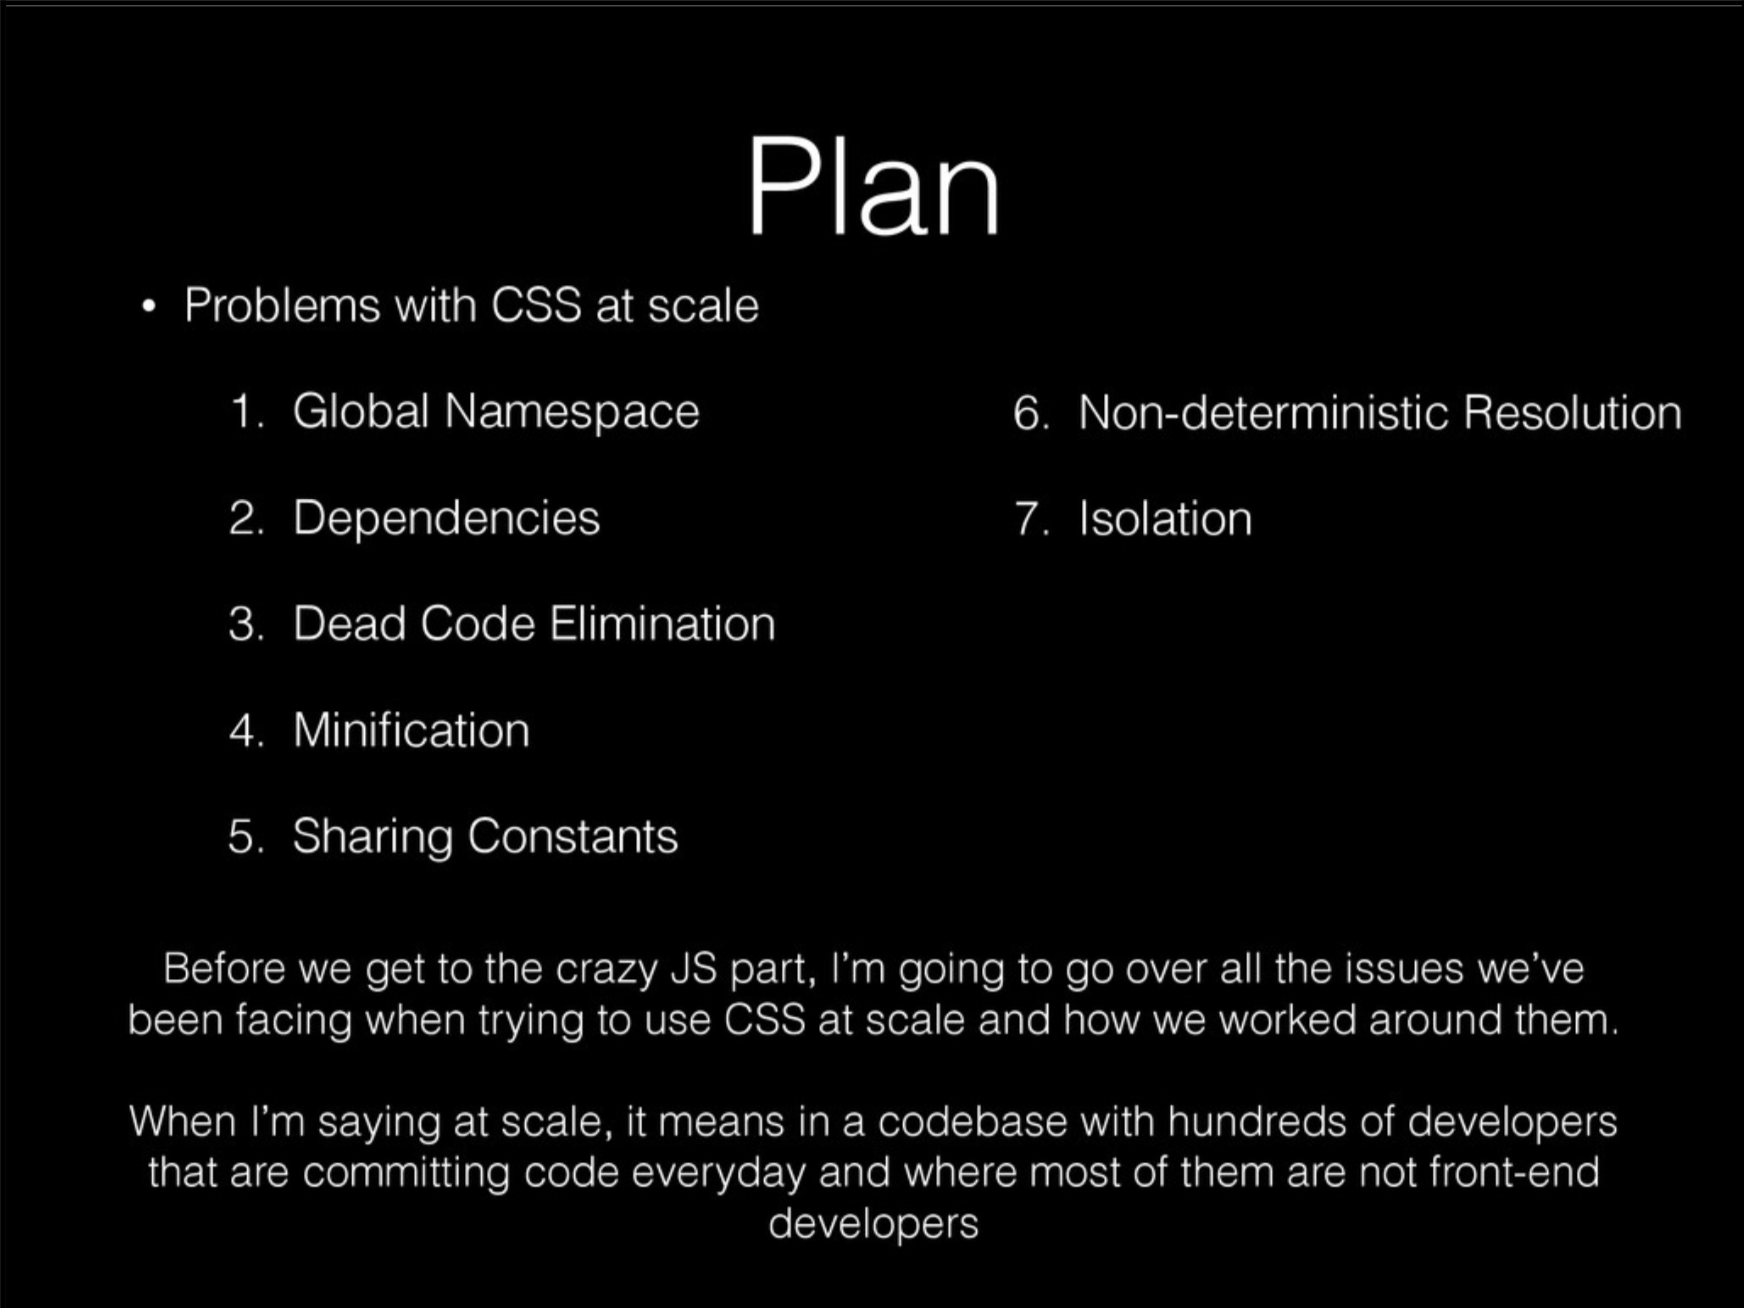
\includegraphics[width=1.\textwidth]{images/css-problems-slide}
\end{figure}

Первая и хорошо известная проблема CSS заключается в глобальных селекторах. Не важно, как вы организовали свой код, использовали ли пространства имен или BEM методологию, в конце все равно стили окажутся в одном глобальном пространстве имен. И это ошибка не только идеологически, это ведет к множеству ошибок и ухудшает поддерживаемость большой кодовой базы. Когда мы работаем в больших командах, не так просто знать о существовании конкретного класса или стилизованного элемента, что ведет к добавлению большего количества классов вместо переиспользования существующих.

Следующая проблема относится к определению зависимостей. На деле бывает очень сложно понять, от каких именно стилей зависит конкретный компонент. Так как стили глобальны, они могут использоваться из любых компонентов, а любой компонент может использовать любые стили. В таких условиях может быть очень легко потерять контроль.

Фронтенд разработчики привыкли использовать препроцессоры для разделения CSS на модули, но в итоге для браузера все равно генерируется большой CSS бандл. Так как объем кода CSS быстро растет, мы получаем еще одну проблему с \textbf{удалением неиспользуемого кода (dead code elimination)}. Так как сложно понять, какой стиль к какому компоненту относится, задача удаления неиспользуемого кода становится еще сложнее. Также, если учесть каскадную природу CSS, удаление любого селектора или правила может привести к непредсказуемым последствиям в браузере.

Минификация селекторов и имен классов также добавляет головной боли и в CSS и в JavaScript приложение. Хотя на первый взгляд эта задача кажется простой, на деле все усложняется, когда классы добавляются во время исполнения программы или высчитываются на клиенте.

Отсутствие возможности минифицировать CSS сильно сказывается на производительности, так как может значительно сказаться на размере CSS файлов.

Также в рамках обычного CSS нетривиально создать константы, общие для CSS и JavaScript. Например для случаев, когда мы хотим знать высоту заголовка, чтобы рассчитать расположение элементов относительно него.

Обычно, JavaScript API используется для получения нужных значений, однако было бы значительно оптимальней использовать общие константы и избежать дорогих вычислений во время исполнения программы. Это и есть пятая проблема, которую Vjeux и другие разработчики Facebook попытались решить.

Шестая проблема заключается в недетерминированный обработке файлов CSS. По факту, в CSS важен порядок обработки файлов с исходниками, поэтому, если файлы грузятся по требованию, то сохранение их порядка не гарантируется, что ведет к применению неверных стилей к компонентам. 

Предположим, что мы хотим оптимизировать загрузку CSS и загружать стили для конкретной страницу только тогда, когда пользователь открывает эту страницу. Если стили, которые относятся к последней странице, содержат правила, которые затрагивают остальное приложение, то отображение всего приложения может измениться. Например, если пользователь вернется по истории к предыдущей странице, она может несколько отличаться от того, что было до этого.

Очень сложно контролировать различные комбинации стилей, правил и путей, но возможность загружать CSS по мере необходимости критична для производительности приложения.

И седьмая проблема, о которой говорит Кристофер Шедо, связана с изоляцией компонент. В CSS очень сложно добиться изоляции файлов или компонентов между собой. Так как селекторы глобальны, они могут быть легко перезаписаны. Это нетривиальная задача, определить финальные стили компонента по примененным к нему классам, так как любой компонент может быть затронут любыми стилями, находящимися в приложении.

Я рекомендую посмотреть это выступление, если вы хотите узнать больше о проблемах масштабируемости CSS. Даже если этот вопрос выглядит сложным и противоречивыми, стоит открыто подходить к нему, чтобы найти решение, которое лучше всего подойдет в вашем случае:

\begin{quotation}
https://vimeo.com/116209150	
\end{quotation}

В заключении этого выступления было сказано, что для решения этих проблем масштабирования CSS в Facebook остановились на использовании \textit{встроенных стилей (inline styles)}.

В следующей части мы рассмотрим, как использовать встроенные стили в React, и какие есть плюсы и минусы у этого подхода.

\section{Встроенные стили}

Документация React советует разработчикам использовать встроенные стили для стилизации компонент. Это выглядит странно, так как за прошедшие годы мы усвоили, что разделение отвественности это хорошо, и мы не должны смешивать разметку и CSS.

React пытается изменить взгляд на разделение ответственности с привычного разделения технологий на разделение компонент. Разделение разметки, стилей и логики на разные файлы, которые сильно связаны и не могут работать по отдельности, иллюзия. Даже если это делает структуру чище, это не приносит реальной выгоды.

В React мы комбинируем компоненты, которые являются базовыми блоками для создания приложения. Мы можем переносить блоки по всему приложению и, независимо от того, где используются компоненты, они должны предоставлять одинаковую логику и отображение.

Это одна из причин, почему объединение стилей с компонентом с помощью встроенных стилей может иметь смысл в React.

Прежде всего посмотрим, как вообще использовать встроенные стили в React компонентах. Создадим кнопку с текстом \textbf{Click me!} и изменим у нее цвета фона и текста:

\begin{lstlisting}
const style = {
  color: 'palevioletred',
  backgroundColor: 'papayawhip',
}

const Button = () => <button style={style}>Click me!</button>
\end{lstlisting}

Как вы видите, использовать встроенные стили очень просто. Нам достаточно создать объект, в котором будут пары ключей и значений как в обычном CSS.

Единственный нюанс, правила с дефисом в названии должны быть записаны в горбатом регистре, а значения передаваться как строки, то есть в кавычках.

Есть несколько отличий при использовании вендорных префиксов. Например, если мы хотим определить переход (transition) в \textbf{webkit}, мы должны использовать атрибут WebkitTransition, который начинается с заглавной буквы. Это правило работает для всех вендорных префиксов кроме \textbf{ms}, которой должен быть в нижнем регистре.

Помимо этого, числа могут использовать без кавычек и единиц измерения, тогда они будут считаться пикселями.

Следующий фрагмент стилей устанавливает высоту в $100px$:

\begin{lstlisting}
const style = {
  height: 100,
}
\end{lstlisting}

Встроенные стили не только прекрасно работают, но и позволяют делать вещи, которые сложно сделать в CSS. Например, мы можем пересчитать значения стилей на клиенте во время исполнения, что мы увидим в следующим примере.

Предположим, что мы хотим создать поле ввода, размер шрифта в котором будет зависеть от его значения. То есть если значение поля будет равно 24, то и размер шрифта должен быть 24 пикселя. Сделать это с помощью CSS невозможно, также нужно приложить значительные усилия, чтобы сделать это в JavaScript.

Посмотрим, как легко сделать это со встроенными стилями.

Нам нужно будет хранить состояние компонента, поэтому создадим для него класс:

\begin{lstlisting}
class FontSize extends React.Component
\end{lstlisting}

В конструкторе класса определим начальное значение компонента, а также привяжем обработчик событий ввода к экземпляру этого класса:

\begin{lstlisting}
constructor(props) {
  super(props)
  
  this.state = {
    value: 16,
  }
  
  this.handleChange = this.handleChange.bind(this)
}
\end{lstlisting}

Мы создадим простой обработчик, который будет только обновлять состояние компонента в соответствии с вводимыми пользователем данными:

\begin{lstlisting}
handleChange({ target }) {
  this.setState({
    value: Number(target.value),
  })
}
\end{lstlisting}

И в конце мы создаем поле ввода с числовым типом, значение которого контролируется нашим компонентом через значение состояния и обработчик событий ввода.

Также мы передадим в атрибут $style$ этого поля ввода объект с актуальным значение размера шрифта. Как говорилось выше название правило должно быть в горбатом регистре, то есть мы должны определить параметр $fontSize$:

\begin{lstlisting}
render() {
  return (
    <input
      type="number"
      value={this.state.value}
      onChange={this.handleChange}
      style={{ fontSize: this.state.value }}
    />
  )
}
\end{lstlisting}

Как мы видим, при изменении значения поля ввода обновляется состояние компонента, что влечет за собой перерисовку компонента. В момент перерисовки значение размера шрифта берется из состояния компонента, которое берется из состояния. Таким образом размер шрифта меняется вслед за значением поля ввода. 

Как и у любого другого решения у встроенных стилей есть свои плюсы и минусы. И в данном случае последних не мало.

Например, со встроенными стилями невозможно использовать псевдоклассы (такие как $:hover$) и псевдоэлементы, что является большим ограничением, если вы хотите создать интерактивный и анимированный UI.

Есть множество костылей (workarounds), которые вы можете использовать для обхода этих ограничений. Например вы можете обычные элементы вместо псевоэлеменов, но для симуляции поведения CSS придется использовать CSS, что не оптимально.

То же самое относится и к \textbf{Медиа запросам (Media queries)}, которые нельзя определить с помощью встроенных стилей, что затрудняет создание адаптивного интерфейса. Также, так как стили передаются через JavaScript объект, во встроенных стилях невозможно использовать style fallbacks:

\begin{lstlisting}
display: -webkit-flex;
display: flex;
\end{lstlisting}

Все из-за того, что JavaScript объекты не могут содержать два атрибута с одинаковым именем. По этой причине использовать style fallbacks невозможно, хотя было бы хорошо иметь возможность их использовать при необходимости.

Еще одна возможность CSS, которую невозможно использовать через встроенные стили, это \textbf{Анимации}. Основной костыль (workaround) в этом случае, определить анимации глобально и использовать их внутри атрибута элементов $style$.

После использования встроенных стилей для предопределения стилей из CSS мы вынуждены использовать ключевое слово $!important$, что является плохой практикой, так как предотвращает применение других стилей к элементу.

И самое ужасное, что происходит при использовании встроенных стилей, это значительное усложнение отладки приложения. Мы вынуждены использовать названия классов для поиска элементов через DevTools браузера в целях отладки и проверки, какие стили были применены.

При использовании встроенных стилей все созданные стили окажутся в атрибуте $tyle$ созданного HTML элемента, что усложняет их отладку.

Например, кнопка из предыдущего примера будет отображена в следующий элемент:

\begin{lstlisting}
<button style="color: palevioletred; background-color: papayawhip;">Click me!</button>
\end{lstlisting}

Один такой такой элемент несложно прочитать, но представьте, что будут сотни таких элементов стилей. В этот момент это начинает превращаться в проблему.

Если вы отлаживаете список таких элементов, в котором у каждого элемента своя копия стилей, то при изменении одного элемента в браузере вы увидите, что меняется только элемент, который вы редактируете, а все соседние элементы остаются неизменными. 

И помимо всего этого, если вы рендерите приложение на стороне сервера (подробнее мы поговорим об этом в Главе 8), то при использовании встроенных стилей размер страницы будет значительно больше. 

Алгоритмы сжатия могут достаточно сильно сжать получившийся HTML, так как в нем будет много повторяющихся частей, в некоторых случаях загрузка критичной части CSS может быть даже хорошей идеей, но в целом мы должны стремиться избежать этого.

Таким образом мы приходим к тому, что встроенные стили создают проблем больше чем решают.

По этим причинам сообщество создало другие инструменты для решения проблем встроенных стилей, не теряя при этом объединения стилей с компонентами. 

После выступления Кристофера Шедо множество разработчиков задумались о проблеме встроенных стилей и начали искать новые решения для использования CSS в JavaScript.

Автор книги изучил все из них и опубликовал репозиторий, в котором создал простую кнопку с помощью каждого из этих методов:

\begin{quotation}
https://github.com/MicheleBertoli/css-in-js
\end{quotation}

В начале их было две или три, но сейчас насчитывается уже больше 40.

В следующих частях мы разберем самые популярные из них.

\section{Radium}

\section{CSS Modules}

\subsection{Webpack}

\subsection{Setting up a project}

\subsection{Locally scoped CSS}

\subsection{Atomic CSS Modules}

\subsection{React CSS Modules}

\section{Styled Components}

\section{Summary}

















\end{document}










